% !TEX program = xelatex
% ===========================================================================
% 格点 QCD 计算质子中胶子 TMD-PDF 的理论解析与工作流（梯度流重整化版）
% 版本: v20260911 —— 基于 PyQCD 已验证代码链的全新版本
% 对照: 理论解析与工作流.tex（过时未验证版，主线为 collinear gluon PDF）
% 编译: cd docs && xelatex 理论解析与工作流-v20260911.tex（两遍）
% 验证简报: 本库 git tag:message（dev14/follow stab24）+ commit 067a777
% ===========================================================================
\documentclass[11pt,a4paper]{ctexart}

% --------------- 页面设置 ---------------
\usepackage[margin=2.4cm]{geometry}
\usepackage{setspace}
\onehalfspacing
\emergencystretch=3em

% --------------- 数学与物理 ---------------
\usepackage{amsmath,amssymb,amsfonts,mathtools}
\usepackage{bm}
\usepackage{braket}
\usepackage{slashed}

% --------------- 图形与颜色 ---------------
\usepackage{graphicx}
\usepackage{xcolor}
\usepackage{tikz}
\usetikzlibrary{arrows.meta, positioning, shapes, decorations.pathmorphing, calc}

% --------------- 表格 ---------------
\usepackage{array,booktabs,multirow,tabularx,longtable}
\setlength{\tabcolsep}{4pt}
\renewcommand{\arraystretch}{1.08}

% --------------- 超链接与 URL ---------------
\usepackage{url}
\usepackage[hidelinks]{hyperref}
\urlstyle{tt}

% --------------- 代码 ---------------
\usepackage{listings}
\lstset{
  basicstyle=\ttfamily\footnotesize,
  breaklines=true,
  frame=single,
  numbers=left,
  numberstyle=\scriptsize\color{gray},
  commentstyle=\color{gray},
  keywordstyle=\color{blue},
  stringstyle=\color{red},
  keepspaces=true,
  columns=flexible,
}

% --------------- 自定义命令 ---------------
\newcommand{\Fmunu}{F_{\mu\nu}}
\newcommand{\Ftmunu}{\tilde{F}_{\mu\nu}}
\newcommand{\Ftzmu}{\tilde{F}^{\mu z}}
\newcommand{\eps}{\varepsilon}
\newcommand{\LaMET}{\text{LaMET}}
\newcommand{\MSbar}{$\overline{\text{MS}}$}
\newcommand{\MSbarM}{\overline{\text{MS}}}
\newcommand{\QCD}{\text{QCD}}
\newcommand{\tr}{\operatorname{Tr}}
\newcommand{\Tr}{\operatorname{Tr}}
\newcommand{\trc}{\operatorname{tr}}
\newcommand{\SU}{\mathrm{SU}}
\newcommand{\diag}{\operatorname{diag}}
\newcommand{\vev}[1]{\langle #1 \rangle}
\newcommand{\abs}[1]{\lvert #1\rvert}
\newcommand{\order}[1]{\mathcal{O}(#1)}
\newcommand{\code}[1]{\texttt{#1}}
\newcommand{\pathref}[1]{\path{#1}}
\newcommand{\GFr}{\mathrm{GF}}
\newcommand{\bperp}{b_{\perp}}
\newcommand{\zzh}{\widehat{\tau}}

% --------------- 验证状态色标 ---------------
\definecolor{goodgreen}{RGB}{30,132,73}
\definecolor{pyblue}{RGB}{36,91,163}
\definecolor{warnorange}{RGB}{197,90,17}
\newcommand{\verified}{\textcolor{goodgreen}{\textbf{已验证}}}
\newcommand{\inferred}{\textcolor{pyblue}{\textbf{推导成立}}}
\newcommand{\unverified}{\textcolor{warnorange}{\textbf{未验证}}}

% --------------- 标题 ---------------
\title{\textbf{格点 QCD 计算质子中胶子 TMD-PDF 的理论解析与工作流}\\[0.4em]
\large —— 梯度流重整化方案的系统化理论整理（已验证版本 v20260911）}
\author{基于 PyQCD 已验证代码链与 donghx 参考实现的系统化整理}
\date{2026 年 9 月 11 日}

\begin{document}

\maketitle

\begin{abstract}
\noindent
本文是格点 QCD 计算\textbf{质子中胶子 TMD-PDF}（transverse-momentum-dependent
parton distribution，基于梯度流重整化方案）的完整理论解析与计算工作流，
为仓库同目录文档 \code{理论解析与工作流.tex}（过时的 collinear-PDF 版本）的
全新替代版本。核心思路是：在蒸馏（distillation）框架下把包含胶子算符的
核子三点关联函数解耦为质子两点函数与纯规范场的非局域胶子算符
（disconnected 通道），对规范组态施加四维 Wilson flow（梯度流，RK3 积分，
$\eps=0.01$）构造流化场强 $F_{\mu\nu}$、对偶场强 $\widetilde F_{\mu\nu}$
与直线 Wilson 线双局域量 $M_{\mu\lambda;\nu\rho}^{\pm}(z)$（schema-v2 六组件
保存），通过关联函数比 $C_3/C_2$（完整复数 \code{pol35} numerator +
共同 \code{nopol} denominator + delete-one jackknife）提取坐标空间矩阵元，
再经小流时间展开（SFTE）的一圈端点转换（Brambilla--Wang
$\GFr\to\MSbarM$）、自重整化 $Z_R$/混合方案、准 TMD-PDF 的 Fourier 重构、
Collins--Soper 核与 NLO 匹配核 $Z_{ij}$ 卷积、软函数/快度减除，最终进行
$a/P_z/m_\pi/L$ 联合外推得到物理 TMD-PDF。

与旧版的关键差异：(1) 主线由 collinear gluon PDF 升级为\textbf{梯度流重整化的
胶子 TMD-PDF}，collinear 通道作为 $\bperp\to 0$ 交叉校验保留；(2) 全部代码
绑定对象由 donghx docker 时代未验证脚本更新为 PyQCD\textbf{已验证}模块链
（schema-v2 OPE、ratio-v2 统计、九项独立契约测试、仓库 106 项全量回归、
与参考估计器逐项 $\max|\mathrm{diff}|=0$ 的数值 oracle）；(3) 新增
「数值结果与验证简报」一章，验证证据以本库 git 标签消息为登记
（\code{dev14}/\code{follow stab24} 与提交 \code{067a777}）；(4) 修复旧版
LaTeX 公式错误、占位 arXiv 编号与重复附录；(5) 重整化主线由 RI/MOM 改为
梯度流方案（$\GFr\to\MSbarM$ 一圈转换 + $Z_R$ 自重整化 + 混合方案 + 比值
方案），RI/MOM 降级为对照。

需要强调的边界：当前已完成的验证终点是\textbf{算法级完整、真实生产级待补
数据}——已交付对象严格称为\textbf{有限流时间 bare disconnected 胶子可观测
量}（schema 状态 \code{flowed\_bare\_ope\_observable}），在补齐参考侧
$L32\times96$、$231$ 组态共同 manifest 生产产物、重整化、混合、软因子、matching 与
连续极限之前，不应称其为已完成的物理胶子 PDF（更不应称物理 TMD-PDF）。
该边界声明贯穿全文并在第 \ref{sec:results} 章系统展开。
\end{abstract}

\tableofcontents
\newpage

% ===========================================================================
\section{QCD 与格点规范场理论基础}
% ===========================================================================

在讨论梯度流重整化的胶子 TMD-PDF 之前，需要建立格点 QCD 的基本理论框架。
本节概述连续时空中的 QCD 拉格朗日量、路径积分量子化方法，以及如何在离散化
的欧几里得时空格点上实现非微扰计算。本节的全部背景约定同样服务于本库
仓库笔记（《格点QCD中的场强张量》《格点QCD中的Wilson线》等，同目录），
符号与 \code{pyqcd} 主包一致。

\subsection{QCD 的拉格朗日量与规范对称性}

量子色动力学（QCD）是描述强相互作用的规范场论，其基本自由度是夸克场
$\psi_f(x)$（味指标 $f = u, d, s, c, b, t$）和胶子场 $A_\mu^a(x)$（色指标
$a = 1,\ldots,8$）。连续时空中的 QCD 拉格朗日量具有 SU(3) 规范对称性：
\begin{equation}
\mathcal{L}_{\text{QCD}} = -\frac{1}{4} F_{\mu\nu}^a F^{a,\mu\nu}
+ \sum_f \bar{\psi}_f (i\gamma^\mu D_\mu - m_f) \psi_f
\end{equation}
其中胶子场强张量定义为：
\begin{equation}
F_{\mu\nu}^a = \partial_\mu A_\nu^a - \partial_\nu A_\mu^a
+ g_0 f^{abc} A_\mu^b A_\nu^c
\end{equation}
协变导数为 $D_\mu = \partial_\mu + i g_0 A_\mu^a T^a$，
$T^a = \lambda^a/2$ 是 SU(3) 生成元，满足对易关系
$[T^a, T^b] = i f^{abc} T^c$。规范变换下场的变换规律为：
\begin{align}
\psi(x) &\to \Omega(x) \psi(x), \quad
\Omega(x) = \exp(i \theta^a(x) T^a) \in \text{SU}(3) \\
A_\mu(x) &\to \Omega(x) A_\mu(x) \Omega^\dagger(x)
+ \frac{i}{g_0} \Omega(x) \partial_\mu \Omega^\dagger(x)
\end{align}
注意本文自始至终区分\textbf{基础表示}（夸克线，Casimir $C_F=4/3$）与
\textbf{伴随表示}（胶子算符的 Wilson 线与 TMD 算符，Casimir $C_A=3$）——
梯度流胶子算符的两端场强由\textbf{伴随表示 Wilson 线}连接，其匹配系数
（第 \ref{sec:matching} 章）因此以 $C_A$ 归一，这是与夸克 PDF 计算
（$C_F$ 归一）最根本的差别之一。

QCD 的两个核心物理特征——\textbf{渐近自由}（高能标下耦合常数变小）和
\textbf{色禁闭}（低能标下色荷被束缚在无色的强子中）——使其低能行为必须
采用非微扰方法处理。

\subsection{路径积分量子化}

在路径积分表述中，物理观测量 $\mathcal{O}$ 的期望值由泛函积分给出：
\begin{equation}
\langle \mathcal{O} \rangle = \frac{1}{Z} \int \mathcal{D}A_\mu
\mathcal{D}\bar{\psi} \mathcal{D}\psi \; \mathcal{O}[A,\bar{\psi},\psi]
\; e^{i S_{\text{QCD}}[A,\bar{\psi},\psi]}
\end{equation}
其中配分函数 $Z = \int \mathcal{D}A_\mu \mathcal{D}\bar{\psi}
\mathcal{D}\psi \; e^{i S_{\text{QCD}}}$，
$S_{\text{QCD}} = \int \mathrm{d}^4 x \, \mathcal{L}_{\text{QCD}}$。

通过 Wick 转动 $t \to -i\tau$（即 $x_0 \to -i x_4$），将 Minkowski 时空转到
Euclidean 时空。此时路径积分中的振荡因子 $e^{iS}$ 变为指数衰减因子
$e^{-S_E}$（$S_E$ 为 Euclidean 作用量），使被积函数变为正定概率权重：
\begin{equation}
\langle \mathcal{O} \rangle_E = \frac{1}{Z_E} \int \mathcal{D}A_\mu
\mathcal{D}\bar{\psi} \mathcal{D}\psi \; \mathcal{O}_E \;
e^{-S_E[A,\bar{\psi},\psi]}
\end{equation}
这一变换是格点 QCD 数值模拟的基础——$e^{-S_E}$ 可以解释为统计力学中的
Boltzmann 权重，允许我们使用 Monte Carlo 方法采样规范组态。

\textbf{Wick 转动与场强的相位约定}对胶子算符尤其重要。采用本库参考实现
的约定（\pathref{refer/donghx/Gradient_Flow_GluonPDF/
gluon_gradient_flow_matching.md}）：Minkowski 度规
$\eta_{\mu\nu}=\mathrm{diag}(1,-1,-1,-1)$、
$\eps_{\mathrm{M}}^{0123}=+1$；代码坐标顺序
$(x,y,z,t)=(0,1,2,3)$、Euclidean
$\eps_{\mathrm{E}}^{xyzt}=+1$。取 Wick 转动
$x^0_{\mathrm{M}}=-i x^t_{\mathrm{E}}$、$A_t^{\mathrm{E}}=-iA_0^{\mathrm{M}}$
，则
\begin{equation}
F^{\mathrm{E}}_{ti}=-iF^{\mathrm{M}}_{0i}, \qquad
F^{\mathrm{E}}_{ij}=F^{\mathrm{M}}_{ij}, \qquad
\widetilde F^{\mathrm{M}}_{0i}=\widetilde F^{\mathrm{E}}_{ti}, \qquad
\widetilde F^{\mathrm{M}}_{ij}=-i\,\widetilde F^{\mathrm{E}}_{ij}
\label{eq:wick-dictionary}
\end{equation}
因此时-电（temporal-electric）与空-磁（spatial-magnetic）项在螺旋度通道中
的 Wick 相位不同。代码中的对偶张量直接使用 Euclidean Levi-Civita 张量；
\textbf{不能}在 OPE 输出之后再额外乘一个 temporal-link 相位。这一约定
是第 \ref{sec:unpol-hel} 节推导非极化/螺旋度算符 Euclidean 结构的基础。

\subsection{格点规范理论}

\subsubsection{Wilson 规范作用量}

格点 QCD 在离散的 Euclidean 时空格点上定义理论。设格距为 $a$，格点坐标为
$x = an$。基本规范自由度由连接 $x$ 到 $x+a\hat{\mu}$ 的\textbf{规范链接}
$U_\mu(x)$ 表示：
\begin{equation}
U_\mu(x) = \mathcal{P} \exp\!\left( i g_0 \int_{x}^{x+a\hat{\mu}}
\mathrm{d}y \, A_\mu(y) \right) \in \text{SU}(3)
\end{equation}
其中 $\mathcal{P}$ 为路径排序算符。最基本的规范不变量是 $1\times 1$
\textbf{Wilson 方格 (plaquette)}：
\begin{equation}
U_{\mu\nu}(x) = U_\mu(x) U_\nu(x+a\hat{\mu})
U_\mu^\dagger(x+a\hat{\nu}) U_\nu^\dagger(x)
\end{equation}
Wilson 规范作用量通过对所有方格求和构造：
\begin{equation}
S_G[U] = \frac{\beta}{3} \sum_x \sum_{\mu<\nu} \operatorname{Re}
\operatorname{Tr}[1 - U_{\mu\nu}(x)]
\end{equation}
其中 $\beta = 6/g_0^2$。在 $a \to 0$ 的极限下，该作用量恢复为连续
Yang-Mills 作用量：
\begin{equation}
S_G = \frac{1}{2g_0^2} \sum_x a^4 \operatorname{Tr}[F_{\mu\nu} F^{\mu\nu}]
+ \order{a^2}
\end{equation}

\subsubsection{费米子作用量与 Clover 改进}

将连续费米子作用量离散化时，朴素离散化会导致 \textbf{fermion doubling}
问题（每个连续费米子产生 16 个格点费米子模式）。Wilson 通过添加量纲为 5
的项（Wilson 项）消除了加倍子，代价是破缺了手征对称性：
\begin{equation}
S_F^{\text{Wilson}} = a^4 \sum_x \bar{\psi}(x) \left(
\sum_\mu \gamma_\mu \tilde{\nabla}_\mu - \frac{a r}{2} \sum_\mu
\nabla_\mu^* \nabla_\mu + m_0 \right) \psi(x)
\end{equation}
其中 $\tilde{\nabla}_\mu$ 是对称格点导数，$\nabla_\mu^*\nabla_\mu$ 是格点
Laplace 算符。Wilson 费米子的截断误差为 $\order{a}$。通过添加
\textbf{Sheikholeslami-Wohlert (Clover) 项}可以实现 $\order{a}$ 改进：
\begin{equation}
S_F^{\text{Clover}} = S_F^{\text{Wilson}} - a^4 \frac{c_{\text{SW}} r}{4}
\sum_x \bar{\psi}(x) \sigma_{\mu\nu} \hat{F}_{\mu\nu}(x) \psi(x)
\end{equation}
其中 $\sigma_{\mu\nu} = \frac{i}{2}[\gamma_\mu, \gamma_\nu]$，
$\hat{F}_{\mu\nu}$ 是格点上的场强张量（其 Clover 构造将在
第 \ref{sec:discret} 节详细讨论），$c_{\text{SW}}$ 是改进系数。本库生产
系综（CLQCD，$\beta=6.20$ 与 $\beta=6.41$ 两类）均采用 Clover 改进的
Wilson 费米子。

\paragraph{Fermion doubling 的机制与 Wilson 项}加倍子的根源在于：对自由
Wilson 费米子作 Fourier 变换，动量空间传播子的分母在 Brillouin 区的
16 个角点（每个方向的分量取 $0$ 或 $\pi/a$，即 $2^4$ 个格点动量）处
同时为零——每个角点都是一个连续费米子的复制品。Wilson 项
$\frac{ar}{2}\sum_\mu\nabla_\mu^*\nabla_\mu$ 在角点处给出正比于
$\sum_\mu(1-\cos p_\mu a)$ 的质量抬升，从而把加倍子推到
$\order{1/a}$ 的重质量处逐出低能谱；其代价是 Wilson 项显式破缺手征
对称性：夸克质量获得可加的重正化（需要调到\textbf{临界质量}
$m_c$ 使 pion 质量趋零），轴矢流不再守恒（提取 $f_\pi$ 等手征量需改进
项，见附录 P）。Clover 项不改变加倍子结构，只消去 $\order{a}$ 的
on-shell 截断误差；$c_{\text{SW}}$ 可由微扰或非微扰（如 Schr\"odinger
泛函方法）确定。

\subsubsection{连续极限与标度设定}

格点 QCD 计算的最终目标是提取连续物理（$a \to 0$）。物理观测量在有限
格距下具有截断误差：
\begin{equation}
\mathcal{O}^{\text{lat}}(a) = \mathcal{O}^{\text{phys}} + c_1 a^n
+ c_2 a^{n+1} + \cdots
\end{equation}
其中 $n=1$（未改进）或 $n=2$（$\order{a}$ 改进后）。标度设定通过选择一个
（或多个）实验已知的物理量来确定格距 $a$，常用的标度设定量包括 Wilson 流
参数 $w_0$、重正子质量 $M_\Omega$、$\pi$ 介子衰变常数 $f_\pi$ 等：
\begin{itemize}
  \item \textbf{Wilson 流参数 $w_0$}（L\"uscher 2010）：由
  $t^2\langle E(t)\rangle|_{t=w_0^2}=0.3$ 定义（$t_0$ 类似但取 0.1 条件
  ），统计与系统误差极小，是目前最广泛使用的标度设定量之一；
  \item \textbf{重正子质量 $M_\Omega$}：$\Omega^-$ 重子质量
  （$1.672$ GeV）对轻夸克质量不敏感，规避手征外推；
  \item \textbf{$\pi$ 介子衰变常数 $f_\pi$}：需注意手征外推的系统误差。
\end{itemize}
不同方法给出的 $a$ 通常在 $\sim1\%$ 内一致，该差异纳入系统误差预算
（附录 Q 汇总单位转换；本库 \code{scale\_setting\_t0} 实现 0.3 目标 +
反插值 + 自动扩围）。

梯度流重整化方案对标度设定有一个自然的附加工具：流观测量
$t^2\langle E(t)\rangle$（$E(t)=\frac14 G^2_{\mu\nu}$）在流时间 $t$ 下的
行为由纯规范动力学位形决定，\code{pyqcd/renorm/\_gradient\_flow.py} 提供
\code{scale\_setting\_t0}（$t^2\langle E(t)\rangle|_{t=t_0}=0.3$ 的 Lüscher
惯例，含反插值与自动扩围）。此外，Wilson flow 的平滑半径
$r_{\mathrm{flow}}=\sqrt{8t}$ 本身提供了一个规范不变的物理长度标度——
这正是梯度流方案把 \textbf{流时间} 当作重整化方案的出发点（第
\ref{sec:renorm} 章）。

\subsection{强子谱学与关联函数}

格点 QCD 中的强子质量通过两点关联函数的大时间行为提取。对于强子插值算符
$\mathcal{O}_H(\mathbf{x}, t)$（具有所需量子数），两点关联函数为：
\begin{equation}
C_2(t) = \sum_{\mathbf{x}}
\langle \mathcal{O}_H(\mathbf{x}, t) \mathcal{O}_H^\dagger(\mathbf{0}, 0)
\rangle
\end{equation}
插入完备的哈密顿量本征态集合后：
\begin{equation}
C_2(t) = \sum_n |\bra{0} \mathcal{O}_H \ket{n}|^2 e^{-E_n t}
\end{equation}
在大时间极限下，基态占主导：
\begin{equation}
C_2(t) \xrightarrow{t \to \infty} |Z_0|^2 e^{-E_0 t}
\end{equation}
由此可以提取强子质量 $E_0 = m_H$（静止系）或
$E_0 = \sqrt{m_H^2 + \mathbf{P}^2}$（运动系）。

在实际计算中，为了增强基态重叠并压制 UV 涨落，需要对夸克场进行
\textbf{涂抹}（smearing）。常用的涂抹方法包括 Jacobi 涂抹、Wuppertal 涂抹
和 Distillation（将在第 \ref{sec:distillation} 节详细讨论）。对本库的
TMD-PDF 生产链，质子两点函数由\textbf{动量涂抹蒸馏}（momentum-smeared
distillation）计算（\pathref{refer/donghx/} 的 \code{2pt\_proton\_*} 系列
脚本，PyQCD 对应 \code{pyqcd/vertex}、\code{pyqcd/contraction} 与
\code{pyqcd/pipeline} 的收缩管线）。

\paragraph{动量投影与色散关系}对运动系计算，插值算符带动量投影
$\mathcal N_\alpha(\mathbf P,t)=\sum_{\mathbf x}
e^{-i\mathbf P\cdot\mathbf x}\mathcal N_\alpha(\mathbf x,t)$，
谱参数化为
$C_2(\Delta t,\mathbf P)=\sum_n Z_n(\mathbf P)e^{-E_n(\mathbf P)\Delta t}$，
$E_n(\mathbf P)=\sqrt{m_n^2+\mathbf P^2}+O(a^2)$。色散关系本身是一个
强检验：用多动量数据拟合 $E(P_z)=\sqrt{m^2+k_2P_z^2+k_3P_z^4a^2}$ 可
同时得到 $m_N$ 与 $a$ 的一致性诊断（\code{pyqcd/analysis/\_dispersion.py}
，移植 zengch \code{fit\_E0} 逻辑；本库实战值：$P_0$ 通道 meff 平台
$\approx1.12$ GeV 与质子质量一致、$P_2$ 通道 $\approx1.56$ GeV 与色散
预期自洽，stab1/dev6/dev7 跨运行互差 3--5 MeV）。有效质量
$m_{\rm eff}(\Delta t)=\ln[C_2(\Delta t)/C_2(\Delta t+1)]$ 在大
$\Delta t$ 趋于平台 $E_0$；激发态污染与信噪比衰减（Parisi-Lepage，第
\ref{sec:statistics} 章）共同决定了平台窗口的选取。

\subsection{夸克传播子与关联函数的计算}

\subsubsection{夸克传播子}

夸克传播子定义为 Dirac 算符的逆：$S(x,y) = D^{-1}(x,y)$。在实际计算中，
对于给定的源 $\eta(y)$，通过求解线性系统得到解 $\psi(x)$：
\begin{equation}
\sum_y D(x,y) \psi(y) = \eta(x), \quad
\psi(x) = \sum_y S(x,y) \eta(y)
\end{equation}
通常使用共轭梯度（CG）类迭代求解器（实矩阵非正定时用 BiCGStab/GCR），
收敛速率由 Dirac 算符的条件数决定——该条件数在接近手征极限
（$m_q \to 0$）时发散，导致\textbf{临界减速}现象。标准缓解手段：
even-odd 预条件（Wilson Dirac 算符的空间奇偶分解使每次迭代成本减半）、
多重格点（multigrid，把低模粗化后求解）、deflation（先投影掉低本征模
再迭代）。截断求解器（达到容差 $\eps$ 即停）引入的偏差可用「精确
relaxed 求解」估计后减除（第 \ref{sec:frontier} 节）。蒸馏框架把传播子
投影到低模子空间后再做收缩（第 \ref{sec:distillation} 节），从统计口径
上绕开了部分临界减速问题。

\subsubsection{点源与涂抹源}

最简单的源是\textbf{点源}：$\eta(y) = \delta_{y,y_0}
\delta_{\alpha\alpha_0} \delta_{aa_0}$，但点源与强子基态的重叠很差。
涂抹源通过在空间上扩展源来增强与物理态的耦合。常用的涂抹源包括：
\begin{itemize}
  \item \textbf{Wall 源}：在固定时间片上，所有空间点取常数值（需要规范固定）；
  \item \textbf{Gaussian 源}：$\eta(x) \propto \exp(-|\mathbf{x} - \mathbf{x}_0|^2
  / (2\sigma^2))$；
  \item \textbf{Jacobi 涂抹源}：通过迭代应用规范协变的 hopping 算符构建。
\end{itemize}

\subsubsection{夸克场双线性算符的 Wick 收缩}

对于形如 $\bar{\psi}(x) \Gamma \psi(x)$ 的定域夸克双线性算符，Wick 收缩给出：
\begin{equation}
\bar{\psi}(x) \Gamma \psi(x) \to -\tr[\Gamma S(x,x)]
\end{equation}
对于非定域的双线性（如 $\bar{\psi}(x) \Gamma W(x,y) \psi(y)$），收缩涉及从
$y$ 到 $x$ 的夸克传播子，中间插入 Wilson 线。

\subsection{格点 QCD 数值模拟的基本流程}

完整的格点 QCD 数值模拟包括以下步骤：
\begin{enumerate}
  \item \textbf{规范组态生成}：使用 HMC (Hybrid Monte Carlo) 算法对 SU(3)
  规范场采样，生成具有概率权重 $e^{-S_E[U]}$ 的规范组态系综；
  \item \textbf{夸克传播子计算}：在固定规范组态上，通过求解 Dirac 方程
  $D[U] \psi = \eta$ 得到夸克传播子；
  \item \textbf{Wick 收缩}：将夸克传播子按照 Wick 定理收缩为所需的强子
  关联函数；
  \item \textbf{统计分析与物理提取}：对组态系综求平均，利用拟合方法提取
  物理观测量（质量、矩阵元等），并进行连续极限和手征外推。
\end{enumerate}

\paragraph{HMC 与组态生成简述}对含费米子的理论，Grassmann 积分给出
$\det D[U]$，其指数化（$\exp[\sum_f\bar\phi D^{-1\dagger}D^{-1}\phi]$
的多伪费米子表示）与分子动力学构成 HMC：蛙跳（leapfrog）积分器保辛、
体积保持且时间可逆，接受率由能量漂移 $\delta H$ 控制；SU(3) 上的指数
映射与力计算在群流形上进行，实践中用多时间尺度积分器与 UV 过滤
（UV-filtered pseudofermions）分离紫外与红外动力学力（方法细节见本库
笔记《格点QCD中的蒙卡方法》）。本库不生成组态——消费合作组提供的
ILDG/Clover 系综（thin link 或已完成涂抹），可直接读取 ILDG
\code{.lime}/\code{.lime.contents}（\code{pyqcd/operator} 的
\code{read\_gauge\_lime}）。

\paragraph{本库生产链的输入数据}蒸馏管线的四类输入数据（维度以本库
张量布局约定为准，tzyx 序）：

\begin{table}[htbp]
\centering
\caption{计算所需输入数据（\code{pyqcd} 布局约定）}
\small
\begin{tabular}{c l l}
\toprule
\textbf{数据类型} & \textbf{说明} & \textbf{维度} \\
\midrule
\code{gauge} & SU(3) 规范链接 $U_\mu(x)$（ILDG 二进制） &
$(N_t,N_z,N_y,N_x,4,3,3)$ \\
\code{eigvecs} & Laplace 本征矢量 $v^{(k)}(x)$ &
$(N_{\text{ev}},\,N_xN_yN_z,\,3)$ \\
\code{peram} & Perambulator $\tau$ & $(N_t,4,4,N_{\text{ev}},N_{\text{ev}})$ \\
\code{VVV} & Baryon block $\Phi_{abc}$ & $(N_{\text{ev}},N_{\text{ev}},N_{\text{ev}})$ \\
\bottomrule
\end{tabular}
\end{table}

典型参数（本库系综，附录 J）：$24^3\times72$ 与 $32^3\times96$ 两类；
$N_{\text{ev}}=100$；动量 $P_z=2\pi n_z/L$（$n_z=0..8$ 蒸馏基线，
$n_z=3..5$ 参考复现）；动量涂抹 $\mathbf{k}$（方向与大小独立于物理
boost）；Wilson 线最大长度 $z_{\max}\le L/2$。IO 约定：本库管线产物
一律 h5py（\code{save\_tensor\_h5}/\code{load\_tensor\_h5}）；donghx
生态的二进制（perambulator 四 Dirac 分量文件、VdV/VVV f8 交错复数）
由 \code{pyqcd/tools/\_io.py} 的专用 reader 消费
（\code{readin\_vdv\_all}/\code{readin\_vvv\_all}，Nev 自探测 + 截断）。

本节建立的理论基础为后续讨论格点胶子 TMD-PDF 计算提供了必要的背景知识。
接下来进入大动量有效理论（\LaMET）与 TMD-PDF 的核心内容。

% ===========================================================================
\section{理论基础：从光锥 PDF 到 TMD-PDF}
\label{sec:theory}
% ===========================================================================

\subsection{光锥 PDF 的定义与物理起源}

\subsubsection{从深度非弹性散射到部分子分布}

部分子分布函数（PDF）的概念起源于对深度非弹性散射（DIS）实验的描述。
在 DIS 过程 $e + p \to e + X$ 中，高能电子通过交换虚光子 $\gamma^*$ 来探测
质子的内部结构。DIS 的双微分截面为：
\begin{equation}
\frac{\mathrm{d}^2\sigma}{\mathrm{d}x_{\text{B}} \mathrm{d}Q^2}
= \frac{4\pi\alpha^2}{x_{\text{B}} Q^4} \left[
\left(1 - y + \frac{y^2}{2}\right) F_2(x_{\text{B}}, Q^2)
- \frac{y^2}{2} F_L(x_{\text{B}},Q^2) \right]
\end{equation}
其中 $x_{\text{B}} = Q^2/(2P\cdot q)$ 为 Bjorken-$x$，$Q^2 = -q^2$ 为虚光子
动量平方，$y = P\cdot q/(P\cdot k)$ 为非弹性度。在 Bjorken 极限下
（$Q^2 \to \infty$，$x_{\text{B}}$ 固定），结构函数 $F_2$ 呈现近似标度无关性
（Bjorken scaling）。根据 QCD 因子化定理，结构函数可以因子化为硬散射截面
（可微扰计算）与 PDF（非微扰）的卷积：
\begin{equation}
F_2(x_{\text{B}}, Q^2) = \sum_{a=q,\bar{q},g} \int_{x_{\text{B}}}^{1}
\frac{\mathrm{d}z}{z} \,
C_{2,a}\!\left(\frac{x_{\text{B}}}{z}, \frac{Q^2}{\mu^2}, \alpha_s(\mu)\right)
f_a(z, \mu^2)
\end{equation}
其中 $f_a(x, \mu^2)$ 是味为 $a$ 的部分子携带纵向动量分数 $x$ 的概率密度，
$C_{2,a}$ 是硬散射系数函数。

\subsubsection{光锥关联函数定义}

在 QCD 的算符形式中，非极化胶子光锥 PDF 的一个常用显式归一化约定为
（本库参考实现 \pathref{refer/donghx/Gradient_Flow_GluonPDF/
gluon_gradient_flow_matching.md} 采用的写法，文献中亦存在把 $x$、$2P^+$
或螺旋度整体 $i$ 因子放到矩阵元定义中的等价写法——这只改变整体归一化/
符号，不改变相对 $(T-S)$ 张量结构）：
\begin{equation}\label{eq:lightcone_pdf}
x\,g(x, \mu^2) = \frac{1}{2\pi P^{+}} \int \mathrm{d}\xi^{-} \,
e^{-i x P^{+}\xi^{-}} \,
\braket{P | F^{+i,a}(\xi^{-}) \, W^{ab}(\xi^{-}, 0) \, F^{+i,b}(0) | P}
\end{equation}
\begin{equation}\label{eq:lightcone_helicity}
x\,\Delta g(x, \mu^2) = \frac{i}{2\pi P^{+}} \int \mathrm{d}\xi^{-} \,
e^{-i x P^{+}\xi^{-}} \,
\braket{P, S_L | F^{+i,a}(\xi^{-}) \, W^{ab}(\xi^{-}, 0) \,
\widetilde{F}^{+i,b}(0) | P, S_L}
\end{equation}
其中：
\begin{itemize}
  \item $P^{+} = (P^{0} + P^{3})/\sqrt{2}$ 为光锥坐标下的正向动量，横向指标
  $i=1,2$（垂直于 $P^+$）；
  \item $\Fmunu$ 为胶子场强张量，$\Ftmunu = \tfrac{1}{2}
  \eps_{\mu\nu\rho\sigma}F^{\rho\sigma}$ 为对偶场强张量；
  \item $W^{ab}(\xi^{-},0)$ 为连接 $\xi^{-}$ 与 $0$ 的光锥 \textbf{伴随表示}
  Wilson 线，确保关联函数的规范不变性：
  \begin{equation}
  W^{ab}(\xi^{-}, 0) = \mathcal{P} \exp\!\left( i g \int_{0}^{\xi^{-}}
  \mathrm{d}\eta^{-} A^{+c}(\eta^{-}) \,(T^c_{\mathrm{adj}})^{ab} \right)
  \end{equation}
  \item $x$ 为 Bjorken-$x$；$\mu$ 为重整化标度，PDF 通过 DGLAP 方程依赖于
  $\mu$。
\end{itemize}
光锥关联函数定义在等光锥时间 $\xi^{+} = 0$ 的超曲面上，这要求理论是
Minkowski 度规的——这是在 Euclidean 格点上直接计算光锥 PDF/TMD 的根本
困难所在。

\subsubsection{Twist 展开与 Leading-Twist 近似}

光锥关联函数可以在 twist 展开的框架下系统分类。算符的 twist 定义为质量
量纲减去自旋：$\tau = d - s$。对于 PDF/TMD，leading-twist（$\tau = 2$）贡献
来自光锥上算符乘积展开的主导项，高 twist（$\tau \geq 3$）修正被 $1/Q^2$
幂次压低。胶子 PDF 的 twist-2 算符就是式~\eqref{eq:lightcone_pdf} 的被积
函数。对于非极化情形，在光锥规范 $A^{+}=0$ 下，Wilson 线化为单位矩阵，
关联函数简化为 $\braket{P | F^{+i}(\xi^{-}) F^{+i}(0) | P}$。

\subsubsection{极化通道的共线定义（螺旋度与横率）}

极化态由场强张量的不同缩并方式区分。非极化算符使用 $F\,W\,F$（两端
均为场强）；螺旋度算符把第二端点替换为对偶张量 $F\,W\,\widetilde F$
（式~\eqref{eq:lightcone_helicity}）；二者的\textbf{对偶差}结构为
\begin{equation}
\Delta\mathcal O(z) \;\propto\;
\bigl(F\,W\,F - F\,W\,\widetilde F\bigr)_{\text{同指标缩并}}
\quad\Longleftrightarrow\quad
\Delta g(x) = \frac12\bigl[g(x,S_L)-g(x,-S_L)\bigr].
\end{equation}
横率（transversity）通道则需要张量结构 $\sigma^{ij}$（chiral-odd）：
\begin{equation}
x\,\delta g(x) \;\leftrightarrow\;
\braket{P,S_\perp|\,F^{\{+i}\,W\,F^{j\}}(0)\,|P,S_\perp},
\end{equation}
其第一阶矩对质子自旋无贡献（chiral-odd 性质），但 TMD 层的
Sivers/Boer--Mulders 结构（附录 S 前沿讨论）使其成为 TMD 自旋物理的
核心。实验提取 $\Delta g$ 对解决质子自旋危机至关重要
（Jaffe--Manohar 分解中的 $\Delta G$）。

\subsubsection{动量求和规则}

胶子 PDF 与夸克 PDF 通过动量求和规则相互关联，反映了强子总动量的守恒：
\begin{equation}
\int_{0}^{1} \mathrm{d}x \, x \left[ \sum_{f} (q_f(x,\mu^2) +
\bar{q}_f(x,\mu^2)) + g(x,\mu^2) \right] = 1
\end{equation}
实验数据显示，在 $\mu^2 \sim 10\;\text{GeV}^2$ 的标度下，胶子携带约
40--45\% 的质子动量。本库对匹配求和规则做过数值断言（对匹配矩阵
$Z_{ij}$ 的对称宽域 $\pm1.9$ 检验，见 \pathref{pyqcd/renorm/AGENTS.md}
的 dev8 对照轮记录——正半轴截断会丢失 $\xi<0$ 支路导致 $+26\%$ 的伪偏移，
且不随 $\mathrm{d}x$ 收敛，故求和规则检验必须覆盖负半轴）。

\subsubsection{Mellin 矩表述与 DGLAP 的矩形式}

PDF 的全部信息等价地编码在 twist-2 定域算符的 forward 矩阵元
（Mellin 矩）中：
\begin{equation}
A^{a}_n(\mu^2) \equiv
\int_0^1 \mathrm{d}x\,x^{n-1}f_a(x,\mu^2)
= \braket{P\big|\mathcal O^{(n)}_a(\mu)\big|P}
\quad(a=q,g),
\end{equation}
其中矩 $A^g_n$ 由胶子能量-动量张量类算符
$\mathcal O_g^{(n)\,\mu_1\cdots\mu_n}
=F^{\{\mu_1\alpha}iD^{\mu_2}\cdots iD^{\mu_n-\}}F_\alpha{}^{\mu_n\rangle}$
给出（$\{\cdots\}$ 对称迹、$\perp$ 无迹化）。\textbf{结构函数的矩
表述}：DIS 的 forward Compton 振幅经 OPE 后
\begin{equation}
T_a(x_B,Q^2) = \sum_n C^a_n\!\left(\frac{Q^2}{\mu^2},\alpha_s\right)
A^a_n\,\frac{1}{x_B^{\,n}},
\end{equation}
Wilson 系数 $C^a_n$ 微扰可算（LO：$C^q_n=\delta$、$C^g_n=0$；
NLO 起出现单态混合）——这正是共线因子化的 Mellin 版本。
\textbf{矩方法的历史局限}（\LaMET{} 前的格点实践）在此再强调一次：
信噪比（信号 $\propto\langle x^{n-1}\rangle$ 随 $n$ 指数下降）、
超立方对称性破缺引起的算符混合与逆 Mellin 不适定性把可靠矩限制在
$n\le3$。\LaMET{} 的突破是把\textbf{矩的离散序列}换成\textbf{坐标
空间连续函数} $h(z,P_z)$——非定域算符在 $z$ 上的形状隐含全部矩。

\subsection{TMD-PDF：横向动量依赖的部分子分布}

\subsubsection{定义与物理意义}

共线 PDF 只描述部分子携带的纵向动量分数 $x$，而 TMD-PDF
（transverse-momentum-dependent PDF）进一步描述部分子\textbf{横向动量
$\mathbf{k}_\perp$} 的分布，提供了强子内部 $(x, \mathbf{k}_\perp)$ 的三维
部分子图像。非极化胶子 TMD 的光锥定义在坐标空间中为（以 $b_\perp$ 为
横向共轭变量）：
\begin{equation}\label{eq:tmd-def}
x\,g(x,\bperp;\mu,\zeta) = \frac{1}{2\pi P^+} \int \mathrm{d}\xi^{-}\,
e^{-ixP^+\xi^{-}}\,
\braket{P|F^{+i}(\xi^- + b_\perp)\, W^{[+\,b_\perp\,+]}\,
F^{+i}(0)|P}_{\mu,\zeta}
\end{equation}
其中 $W^{[+\,b_\perp\,+]}$ 是「纵向 + 横向翼 + 纵向」的 staple 型 Wilson
线。与共线 PDF 的本质区别在于：

\begin{enumerate}
  \item \textbf{额外的过程依赖减除}：TMD 的腰奇点（rapidity divergence）
  要求引入 Collins--Soper 标度 $\zeta$ 与软因子 $S(b_\perp,\mu)$——TMD
  定义依赖 $(\mu,\zeta)$ 双标度，而共线 PDF 只依赖 $\mu$；
  \item \textbf{CS 演化方程}：TMD 随 $\zeta$ 的演化由 Collins--Soper 核
  $K(b_\perp,\mu)$ 驱动，随 $\mu$ 的演化由 DGLAP 型反常量纲 $\gamma_\zeta$
  驱动；
  \item \textbf{单侧（one-sided） staple}：格点上 TMD 算符的 Wilson 线
  在横向方向带一个翼（第 \ref{sec:discret} 节的
  \code{staple\_wilson\_line}），其在 $b_\perp\to0$ 极限下约化为直线
  Wilson 线的共线算符。
\end{enumerate}

\subsubsection{Collins--Soper 演化与软因子}

TMD 矩阵元满足双标度演化方程：
\begin{align}
\frac{\mathrm{d}}{\mathrm{d}\ln\sqrt{\zeta}}\,
\ln F(x,\bperp;\mu,\zeta) &= K(\bperp,\mu), \\
\frac{\mathrm{d}}{\mathrm{d}\ln\mu}\, K(\bperp,\mu)
&= -\gamma_\zeta(g(\mu)),
\end{align}
其中 $K(b_\perp,\mu)$ 是 Collins--Soper 核（快度反常量纲），
$\gamma_\zeta$ 是其 $\mu$ 反常量纲。软因子 $S_I(b_\perp,\mu)$（内禀软
函数）吸收腰发散，使组合量
$F(x,b_\perp) \cdot \sqrt{S_I(b_\perp)}/\sqrt{S(b_\perp)}$ 达到有限的
物理定义。在格点方案中，$K$ 与 $S_I$ 都可以从\textbf{准 TMD 矩阵元的
动量比值}中提取（第 \ref{sec:matching} 章的 LPC 2020 方案与
\code{pyqcd/renorm/\_tmdextract.py} 的 \code{cs\_kernel\_*} 实现）。

\subsubsection{腰发散与格点处理}

在光锥/准 TMD 算符的微扰展开中，腰奇点表现为 $\ln(P_z)$ 型增强项。格点
上的准 TMD 矩阵元 $h_R(z,\bperp,P_z)$ 在大 $P_z$ 下含有
$\exp[\tfrac12 K(b_\perp)\ln(\zeta'_{z}/\zeta)]$ 型的快度演化因子——这是
\textbf{物理的}（CS 演化）与\textbf{腰发散}（需要软减除）的共同来源，
必须通过软函数/快度减除分离，不能简单当作统计噪声（第
\ref{sec:matching} 章的 \code{tmd\_matching\_hybrid} 实现）。

\subsubsection{TMD 因子化定理（SIDIS/DY 结构）}

TMD 的物理定义由半包容深度非弹性散射（SIDIS）与 Drell--Yan 过程的
因子化定理给出。以 SIDIS 为例，其截面在 $q_\perp\ll Q$ 区域因子化为：
\begin{equation}\label{eq:tmd-factorization}
\frac{\mathrm{d}\sigma^{\rm SIDIS}}{\mathrm{d}x\,\mathrm{d}y\,
\mathrm{d}^2 q_\perp}
= \sum_b H_b(x_B,Q,\mu)\,
\int \mathrm{d}^2\bperp\,\frac{\delta(\bperp^2+q_\perp^2/4)}
{\bperp^2}\,
F_{b/h}(x,\bperp;\mu,\zeta)\,
\tilde S_{\rm soft}(\bperp;\mu)
+ \order{q_\perp/Q},
\end{equation}
其中 $H_b$ 是微扰硬系数，$F_{b/h}$ 是目标 TMD（含 CS 演化的
$(\mu,\zeta)$ 依赖），$\tilde S_{\rm soft}$ 是过程无关的软因子——
腰发散在 $F$ 与 $S_{\rm soft}$ 中以相反符号出现，其组合
$F\cdot\sqrt{S_I}/\sqrt{S}$ 有限。Drell--Yan 的结构相同（方向相反的
staple 与符号）。该定理给出了格点准 TMD $\to$ 光锥 TMD 匹配核必须
同时处理的三个成分：硬核 $C$（LaMET 层）、软减除（$S_I$）与 CS 演化
（$K$）——本库下游链的分工即按此三层设计（式
~\eqref{eq:matching_tmd}）。快度标度的自然选择为
$\zeta\sim(2P_z)^2$（格点动量的能量标度），偏离时由
$\exp[\tfrac12 K\ln(\zeta_z/\zeta)]$ 因子衔接。

\subsection{大动量有效理论（\LaMET）}

\subsubsection{Feynman 部分子模型与无穷动量框架}

部分子物理学的现代理解始于 Feynman 的部分子模型：在高能散射中，快速运动
的强子可以视为一束近乎自由的、无相互作用的部分子，每个部分子携带强子
纵向动量的一部分 $x = k_z/P_z$。部分子模型成立的物理条件是\textbf{时距
缩短}：在 IMF 中，强子时间膨胀使散射过程发生在远小于强子束缚时间的时间
尺度上，末态相互作用（最终相互作用定理）对分布观测量的修正被压低；从
Weinberg 的无穷动量微扰理论角度，IMF 中 QCD 的真空简化，强子态可以
展开为自由 Fock 空间中的多部分子态。然而 IMF 形式化存在数学困难：无穷
大动量和 UV 截断的极限不可交换。这一「极限不可交换」正是准分布中
$\ln(P_z)$ 型增强项与快度依赖的来源——它们不是需要除掉的噪声，而是
需要\textbf{被正确重整化}的物理。
\LaMET{} 通过将 IMF 替换为有限但足够大的动量 $P_z$ 来解决这一困难，与
重夸克有效理论（HQET）将无穷大夸克质量替换为有限大夸克质量的策略完全
类似。

\subsubsection{LaMET 与 HQET 的类比}

HQET 与 \LaMET{} 都是处理含有一个大标度的物理系统的有效场论方法：

\begin{center}
\begin{tabular}{c|c|c}
\toprule
\textbf{特征} & \textbf{HQET} & \textbf{LaMET} \\
\midrule
大标度 & 重夸克质量 $m_Q$ & 强子动量 $P_z$ \\
展开参数 & $1/m_Q$ & $1/P_z$ \\
有效理论 & HQET 拉格朗日量 & 部分子模型/光锥关联 \\
匹配因子 & $Z(m_Q/\Lambda, \Lambda/\mu)$ & $Z(P_z/\Lambda, \Lambda/\mu)$ \\
幂次修正 & $\order{1/m_Q}$ & $\order{\Lambda_{\text{QCD}}^2/P_z^2}$ \\
\bottomrule
\end{tabular}
\end{center}

在 HQET 中，包含重夸克的物理观测量 $O(m_Q)$ 在大质量极限下展开为：
\begin{equation}
O(m_Q/\Lambda) = Z(m_Q/\Lambda, \Lambda/\mu) \, o(\mu)
+ \order{1/m_Q} + \cdots
\end{equation}
其中 $o(\mu)$ 是 HQET 中的算符矩阵元，$Z$ 是微扰可计算的匹配系数
——匹配系数的计算方式（计算同一物理量在有效理论与完整理论中的
表达式差）与 \LaMET{} 的匹配核完全同构。

在 \LaMET{} 中，格点上依赖于大动量 $P_z$ 的观测量 $F(P_z/\Lambda)$ 在
大动量极限下展开为：
\begin{equation}\label{eq:lamet_expansion}
F(P_z/\Lambda) = Z(P_z/\Lambda, \Lambda/\mu) \, f(\mu)
+ \order{\frac{\Lambda_{\text{QCD}}^{2}}{P_z^{2}}}
\end{equation}
其中 $f(\mu)$ 是 $P_z \to \infty$ 时的光锥观测量（即部分子分布），
包含所有红外共线发散。\textbf{这意味着：Feynman 的部分子模型实际上就是
大动量强子的有效理论。}

\subsubsection{因子化定理的形式与匹配核变元}

对于 TMD 通道，因子化公式中匹配核的独立变元为 $x/y$ 和
$\mu/(yP_z)$（匹配核依赖于部分子动量 $yP_z$ 而非强子动量 $P_z$——这一
精细区别由 Izubuchi、Ji 等人于 2018 年阐明）：
\begin{equation}\label{eq:lamet_factorization}
\tilde{g}(x, P_z) = \int_{-1}^{1} \frac{\mathrm{d}y}{|y|} \,
C\!\left(\frac{x}{y}, \frac{\mu}{|y|P_z}\right) \,
g(y, \mu) + \order{\frac{\Lambda_{\text{QCD}}^{2}}{P_z^{2}},\;
\frac{\Lambda_{\text{QCD}}^{2}}{x^{2}P_z^{2}}}
\end{equation}

\subsubsection{因子化定理的 OPE 推导}

准 PDF 到光锥 PDF 的匹配关系可以通过算符乘积展开严格推导。考虑坐标空间
中的重整化 Wilson 算符 $O(z,\mu)$，在短距离极限 $z \to 0$ 下，其 OPE
展开为定域 twist-2 算符的线性组合：
\begin{equation}
O(z, \mu) = \sum_n C_n(\mu^2 z^2) \, \frac{(-iz)^n}{n!} \,
e_{\mu_1}\cdots e_{\mu_n} \, \mathcal{O}_n^{\mu_1\cdots\mu_n}(\mu)
+ \cdots
\end{equation}
其中 $\mathcal{O}_n$ 是 twist-2 的定域算符，Wilson 系数 $C_n$ 在
$\MSbarM$ 方案下微扰可计算。非定域算符的短距离行为完全由定域 twist-2
算符决定，而后者的 forward 矩阵元恰是 PDF 的 Mellin 矩来源——坐标
空间关联函数与动量空间分布由此一一对应。展开的系统性来自渐近自由：
当 $P_z$ 很大时，$F$ 对 $P_z$ 的依赖是可微扰计算的；对固定格距的格点
计算，先取 $a \to 0$ 得到连续极限，再在 $P_z \gg \Lambda_{\rm QCD}$
条件下展开。

\paragraph{Mellin 空间的匹配核结构}把 OPE 与 Fourier 变换结合：对
式~\eqref{eq:lamet_factorization} 取 Mellin 矩，卷积化为乘积，匹配核
在矩空间的行为揭示其结构：
\begin{equation}\label{eq:mellin-kernel}
\tilde g_N(P_z/\mu) = \int_0^1\mathrm{d}y\,y^{N-1}\,
\tilde g(y,P_z) = C_N\!\left(\frac{P_z}{\mu}\right) g_N(\mu)
+\order{\frac{\Lambda^2}{P_z^2}},
\end{equation}
其中 LO 部分是\textbf{动量守恒的} $C_N^{(0)}=1$（对应 $x$ 空间的
$\delta(1-\xi)$）；NLO 部分
$C_N^{(1)}\sim\frac{\alpha_sC_A}{2\pi}
\bigl[\ln(P_z^2/\mu^2)+c_N\bigr]$——$\ln(P_z)$ 的系数矩阵即准算符的
反常维数（其单圈形式在 $x$ 空间给出 $g_1/g_2/g_3$ 三分区核）。这一
「矩空间看结构、$x$ 空间做卷积」的双视角是理解匹配核
plus-distribution 与端点奇点来源的最短路径（数值实现按
式~\eqref{eq:zij-matrix} 的 $Z^{-1}$ 矩阵自然处理）。

\subsubsection{幂次修正的系统分析}

LaMET 的幂次修正来自多个来源：
\begin{enumerate}
  \item \textbf{靶质量修正}：有限质子质量 $M_N$ 导致的修正，量级为
  $\order{M_N^2/P_z^2}$；
  \item \textbf{高 twist 修正}：量级为 $\order{\Lambda_{\text{QCD}}^2/P_z^2}$；
  \item \textbf{小 $x$ 区域的增强修正}：量级为
  $\order{\Lambda_{\text{QCD}}^2/(x^2 P_z^2)}$。
\end{enumerate}
对于典型的格点动量 $P_z \sim 1.5\text{--}2.5$ GeV 和
$\Lambda_{\text{QCD}} \sim 0.3$ GeV，幂次修正的量级约为
$(\Lambda_{\text{QCD}}/P_z)^2 \sim 1.5\%\text{--}4\%$。\textbf{收敛性判据}：
对于可信的 PDF/TMD 提取，需要 $P_z \gtrsim 1.5$ GeV 且
$x P_z \gg \Lambda_{\text{QCD}}$。

\subsubsection{大动量重整化群方程与解析延拓}

匹配因子 $Z(P_z/\Lambda, \Lambda/\mu)$ 满足重整化群方程：
\begin{equation}
\frac{\partial F(P_z)}{\partial \ln P_z} = \gamma(\alpha_s) F(P_z)
+ \order{\frac{1}{P_z^{2}}},
\qquad \gamma(\alpha_s) = \frac{1}{Z}\frac{\partial Z}{\partial \ln P_z}
\end{equation}
利用该方程可对 $P_z$ 的大对数进行重求和，提高微扰匹配的精度——这在
$P_z$ 只能取离散格点动量（$2\pi n_z/L$）的实践中尤为重要：把已知的
$\gamma$ 用来把矩阵元从一对 $P_z$ 演化到另一对，可以检验数据与
$\ln P_z$ 行为的一致性（本库 CS 核提取 \code{cs\_kernel\_*} 正是
$\partial\ln h/\partial\ln P_z$ 的两动量差分实现，见第
\ref{sec:matching} 章）。

\LaMET{} 的关键理论要素是：Euclidean 格点计算能够捕获正确的 Minkowski
光锥物理——解析延拓证明的要点是：考虑一个典型的单圈 Feynman 积分，
Minkowski 版本 $I_M$ 具有共线发散（部分子质量 $m\to0$ 时），Euclidean
版本 $I_E$ 在解析延拓 $p_\tau \to -i p_0$ 后满足 $I'_E = -i I_M$；
两者共享全部共线奇点，差异仅在 UV 区域。格点 QCD 在有限 $P_z$ 下计算的
非局域关联函数包含了与光锥分布相同\textbf{红外物理}，UV 差异可由微扰
匹配核弥补。

\subsection{坐标空间矩阵元：quasi 通道的核心量}

无论是共线 PDF 还是 TMD-PDF，格点计算的直接对象都是\textbf{坐标空间
双局域矩阵元}。对照旧文档的 Eq.~(20) 锚点，本库的统一记号为：
\begin{equation}\label{eq:matrix-element}
\boxed{\;h(z, P_z) \equiv
\frac{\braket{P | \mathcal{O}(z) | P}}{\braket{P|P}}\;}
\end{equation}
其中 $\mathcal{O}(z)$ 在共线通道为直线 Wilson 线连接的胶子双局域算符
（第 \ref{sec:unpol-hel} 节的 $M_{\mu\lambda;\nu\rho}(z)$），在 TMD 通道
为 staple Wilson 线连接的横向分离双局域算符
$h_R(z,\bperp,P_z)$（第 \ref{sec:discret} 节）。矩阵元通过
$C_3/C_2$ 关联函数比提取（第 \ref{sec:factorization} 节）：

\begin{equation}\label{eq:ratio-def}
h^{\text{lat}}(z, P_z; t_{\text{sep}})
= \frac{C_3(t_{\text{sep}}; z, P_z)}{C_2(t_{\text{sep}}; P_z)}
\;\xrightarrow{t_{\text{sep}} \to \infty}\; h(z, P_z)
\end{equation}

\textbf{推导要点（Fourier 重构的 Jacobian 来源）}：上述 Fourier 变换
关系来自把光锥关联函数中沿光锥方向 $\xi^-$ 的积分替换为沿空间方向 $z$
的积分。在 IMF 中 Lorentz 收缩效应使得 $\xi^- \sim z/\gamma$（其中
$\gamma = P_z/M$），坐标空间的纵向动量共轭变量相应地从光锥动量分数
变为 $xP_z$，Fourier 变换核需要乘以 Jacobian 因子 $1/(xP_z)$——
这就是式~\eqref{eq:quasi-pdf-sin} 中 $2P_z/x$ 前因子与式
~\eqref{eq:quasi-tmd} 中 $1/(2\pi P_z)$ 归一的来历。归一化常数
$\mathcal N=P_z^2/P_t^2$ 则来自把光锥 $P^+$ 换成能量分量 $P_t$ 的
运动学修正（准通道中核子的能量-动量关系 $P_t=\sqrt{M_N^2+P_z^2}$）。

\paragraph{向 GPD/形状因子的推广}\LaMET{} 框架可直接推广到
广义部分子分布（GPD）：把零动量插入 $\sum_{\mathbf y}$ 换成
$\sum_{\mathbf y}e^{-i\boldsymbol\Delta\cdot\mathbf y}$（附加动量
$\boldsymbol\Delta$），双局域矩阵元分解为
\begin{equation}
\braket{P'|O(z)|P} = \bar u(P')\bigl[\gamma^{\{\mu_1}\cdots\}
A(z,\Delta^2) + \sigma^{\mu_1\mu_2}\Delta_{\mu_2}\cdots
+\cdots\bigr]u(P),
\end{equation}
不变振幅 $A(z,\Delta^2)$、$B(z,\Delta^2)$ 在 $z\to0$ 极限给出
形状因子（$\Delta^2$ 的连续函数）与能量-动量张量的矩阵元
（ $D$-项、角动量分解）——把 $z$ 依赖（PDF）与 $\Delta^2$ 依赖
（三维层析）联合构造是 LaMET 的下一个自然扩展（本库未实现，列为
方向）。同一算符族还能给出夸克/胶子的角动量分解检验，与
$\Delta G$（第 \ref{sec:frontier} 节）共同构成质子结构的完整拼图。

\subsection{quasi-PDF / quasi-TMD 与匹配关系}

\subsubsection{Fourier 重构}

共线通道的胶子 quasi-PDF 采用反对称（sin）变换：
\begin{equation}\label{eq:quasi-pdf-sin}
\tilde{g}(x, P_z) = \frac{2P_z}{x} \int_{0}^{z_{\text{max}}}
\mathrm{d}z \; h_R(z, P_z) \, \sin(x P_z z)
\end{equation}
（\code{pyqcd/renorm/\_tmdextract.py} 的 \code{quasi\_pdf\_gluon}，
$x\approx0$ 处以 $\abs{x}<10^{-15}$ 守卫置零，与 zhangxin 原版
\code{gluon\_pdf\_full\_workflow.py} 梯形法等价。）

\textbf{sin 与 cos 两通道的物理分工}：sin 变换作用于矩阵元的
\textbf{反对称部分}（$h(z)-h(-z)$，即非极化共线 PDF 的结构通道）；cos
变换（准 TMD 通道，式~\eqref{eq:quasi-tmd}）作用于\textbf{Hermitian
对称部分}（$h(z)+h(-z)$ 经复数 Hermitian 延拓）。两条通道共享同一
$h_R(z)$ 数据但 Fourier 核不同，因此互为\textbf{交叉校验通道}：
$b_\perp$ 积分极限下 TMD 归一到共线 PDF，两通道的数值一致性检验
（同 $x$ 网格、同归一约定）是 Fourier 层实现正确性的强检查。

TMD 通道的准 TMD-PDF 采用余弦型变换并带能量归一因子：
\begin{equation}\label{eq:quasi-tmd}
x\,\tilde{g}(x, \bperp, P_z) = \frac{1}{\mathcal{N}}
\int \frac{\mathrm{d}z}{2\pi P_z}\,
e^{-ixzP_z}\,h_R(z, \bperp, P_z),
\qquad \mathcal{N} = \frac{P_z^2}{P_t^2}
\end{equation}
其中 $P_t = \sqrt{M_N^2 + P_z^2}$ 是核子能量分量。正半轴数据按
$h_R(-z) = h_R(z)^*$ 作 Hermitian 延拓，等价于
$\int_{-L}^{L}dz\,e^{-ikz}h(z) = 2\int_0^L dz\,[\cos(kz)\operatorname{Re}h
+ \sin(kz)\operatorname{Im}h]$（\code{quasi\_tmd\_pdf} 实现，含批量 GEMM
加速——dev8 对照轮把逐列循环批量化为单次矩阵乘法，提速 7.8--68 倍且
逐位一致）。

\subsubsection{赝 PDF / pseudo-ITD 的等价表示}

准 PDF/准 TMD 与赝 PDF/pseudo-ITD 是\textbf{同一空间关联函数}的两种
表示——分别对应 Fourier 变换到 $xP_z$ 空间与 Ioffe 时间
$\nu = zP_z$ 空间：
\begin{equation}
\mathcal{P}(x, z^2) = \int \frac{\mathrm{d}\nu}{2\pi} \, e^{-i x \nu}
\, \mathcal{M}(\nu, z^2)
\end{equation}
Izubuchi、Ji、Jin、Stewart 和 Zhao（2018）严格证明了两种表示满足等价的
因子化公式。对 TMD 通道，reduced pseudo-ITD
$\mathfrak M(\nu,z^2,\mu)=\mathcal M(\nu,z^2,\mu)/\mathcal M(0,z^2,\mu)$
在短距离 OPE 下匹配到光锥 ITD $\mathfrak I_g$/$\Delta\mathfrak I_g$
（channel-specific 核，见 \pathref{refer/donghx/Gradient_Flow_GluonPDF/
gluon_gradient_flow_matching.md} §7.3）。本库实现以 quasi-Fourier 为主
通道，pseudo-ITD 作为交叉校验层保留在文档中。两种表示的对照：

\begin{center}
\begin{tabular}{c c c}
\toprule
\textbf{分布} & \textbf{Fourier 共轭} & \textbf{匹配核变元} \\
\midrule
空间关联 $h(z,P_z)$ & --- & $\zeta=zP_z$、$z^2$ \\
准 PDF/准 TMD & $z \to xP_z$ & $x/y$、$\mu/(yP_z)$ \\
赝 PDF/pseudo-ITD & $\zeta \to x$ & $x/y$、$\mu^2z^2$ \\
\bottomrule
\end{tabular}
\end{center}
两者共享同一格点数据与同一红外物理，提供互补的系统误差交叉检验；
赝 PDF 避开了 Fourier 截断的 Gibbs 振荡（但需小 $z^2$ 外推），
准 PDF 直接给出 $x$ 依赖（但受 $z_{\max}$ 截断限制）。

\subsubsection{NLO 匹配核的数学结构}

quasi 通道到光锥通道的 NLO 匹配关系为：
\begin{equation}
\tilde{g}(x, P_z) = g(x, \mu) + \frac{\alpha_s C_A}{2\pi}
\int_{x}^{1} \frac{\mathrm{d}y}{y} \,
\Delta C_{gg}\!\left(\frac{x}{y}, \frac{\mu}{P_z}\right) g(y, \mu)
+ \cdots
\end{equation}
其中 $\Delta C_{gg}$ 包含 plus-distribution、$\delta(1-\xi)$ 项与
$\ln(\mu^2/P_z^2)$ 对数项；单圈核 $g_0\ldots g_3$ 的显式三分区表达式与
矩阵实现 $Z_{ij}$ 见第 \ref{sec:matching} 章。

\paragraph{NLO 匹配的数值意义}取 $\alpha_s(\mu=2\;\text{GeV}) \approx
0.30$，匹配修正量级约为 $\alpha_s C_A/(2\pi) \sim 14\%$（对照旧文档以
$\alpha_s/(2\pi)\sim4\%$ 估计夸克通道；胶子通道的色因子 $C_A=3$ 使其
约大三倍），在中等 $x$ 区域（$0.1<x<0.5$）可控。区域特异性：
\begin{itemize}
  \item \textbf{大 $x$}：$\xi\to1$ 时出现大对数 $\ln(1-\xi)$，微扰展开
  失效，需要阈值重求和恢复收敛性；
  \item \textbf{小 $x$}：$1/x$ 型增强项放大修正量级
  （$\order{\Lambda^2/(x^2P_z^2)}$），同样需要重求和或谨慎外推；
  \item \textbf{标度变异}：以 $\mu\in[P_z/2,2P_z]$ 的变异估计微扰不确
  定性（第 \ref{sec:systematics} 章）。
\end{itemize}
重要的是，匹配核 $C_{gg}(x/y,\mu/P_z)$ 仅依赖部分子动量比与标度比，
与外部强子态无关——这是因子化定理的核心结论，也意味着匹配核可以
独立于物理目标（核子/介子）复用。

% ===========================================================================
\section{梯度流与格点离散化}
\label{sec:discret}
% ===========================================================================

本章把连续理论映射到格点实现，核心新内容是\textbf{梯度流（Wilson flow）}
作为规范场预处理器与重整化方案入口，以及在此基础上构造的流化场强、
对偶场强、直线 Wilson 线与 TMD staple 算符。实现入口：
\pathref{pyqcd/renorm/_gradient_flow.py}（流引擎）、
\pathref{pyqcd/operator/_gluon_ope.py}（Clover/对偶/legacy OPE）、
\pathref{pyqcd/operator/_gradient_flow_gluon_ope.py}（schema-v2 OPE）、
\pathref{pyqcd/renorm/_tmd.py}（TMD staple）。

\subsection{梯度流：耗散的规范场演化}
\label{sec:flow}

\subsubsection{流方程与平滑半径}

连续 Euclidean 流场 $B_\mu(\tau,x)$ 满足
\begin{equation}
\partial_\tau B_\mu(\tau,x)=D_\nu G_{\nu\mu}(\tau,x),
\qquad B_\mu(0,x)=A_\mu(x),
\end{equation}
它把四维规范场沿作用量下降方向平滑；在正流时间，半径约为 $\sqrt{8\tau}$
的紫外涨落被压制（Lüscher 2010，arXiv:1006.4518）。自由场极限中流化的
规范场带来 $e^{-\tau k^2}$ 阻尼，两端的场强双局域量因此带来
$e^{-2\tau k^2}$——这是\textbf{四维}动量的阻尼；若只在三维空间流化，
匹配系数必须重新计算，不能使用四维 flow 的系数。

\subsubsection{六 staple 与流生成元}

格点上用链接 $V_\mu(\tau,x)$ 表示流场，Wilson 作用量的六个 staple 给出
\begin{equation}\label{eq:staple}
\Omega_\mu(x)=\sum_{\nu\ne\mu}
\Bigl[
U_\nu(x)U_\mu(x+\hat\nu)U_\nu^\dagger(x+\hat\mu)
+U_\nu^\dagger(x-\hat\nu)U_\mu(x-\hat\nu)
U_\nu(x-\hat\nu+\hat\mu)
\Bigr]
\end{equation}
流右端首先形成 $\Omega_\mu V_\mu^\dagger$，再取无迹反厄米部分：
\begin{equation}\label{eq:flow-generator}
Z_\mu(V)=P_{\rm ah}\!\left[\Omega_\mu V_\mu^\dagger\right],
\qquad
P_{\rm ah}(X)=\frac{X-X^\dagger}{2}
-\frac{\tr(X-X^\dagger)}{2N_c}\,\mathbf 1
\end{equation}
因此 $Z_\mu\in\mathfrak{su}(3)$，$\exp(\epsilon Z_\mu)\in\SU(3)$。实现中
\code{su3\_exp} 采用小步长四阶截断并做 determinant 归一（\code{proj\_su3}
），随后以幺正性和 determinant 误差作守卫。实际代码把每一 staple 项按
矩阵乘法写成正、负两个三段路径，并预计算整场 roll（\code{staple\_6} 的
$R_p/R_m$ 缓存，比逐 $(\mu,\nu)$ 独立 roll 快约 1.5--1.8 倍，数学结果
逐位一致，验证 $\max|\mathrm{diff}|=0$）。

\subsubsection{三阶 Runge--Kutta 积分}

Lüscher 三阶更新为
\begin{align}
W_0&=V_\tau, \notag\\
W_1&=\exp\!\left(\frac{\eps}{4}Z_0\right)W_0, \notag\\
W_2&=\exp\!\left(\frac{8\eps}{9}Z_1-\frac{17\eps}{36}Z_0\right)W_1, \notag\\
V_{\tau+\eps}
&=\exp\!\left(\frac{3\eps}{4}Z_2-\frac{8\eps}{9}Z_1
+\frac{17\eps}{36}Z_0\right)W_2.
\label{eq:rk3}
\end{align}
当只给出无量纲流时间 $\zzh=\tau/a^2$ 与步长 $\eps$ 时，步数为
\begin{equation}
N_{\rm step}=\left\lceil\frac{\zzh}{\eps}\right\rceil,
\qquad \delta t=\frac{\zzh}{N_{\rm step}}
\end{equation}
最后一步使用 $\delta t$ 而非盲目使用 $\eps$，故实际流时间恰好命中目标
（\code{wilson\_flow} 实现；显式传入 $N_{\rm step}$ 时 metadata 同时保存
用户步数与真实步长）。生产参考约定为 $\eps=0.01$（契约测试同时验证
$\eps=0.01$ 对 $\eps=0.005$ 的相对差约 $3.1\times10^{-6}$，量级符合三阶
积分预期）。

\subsubsection{流时间量纲与三套记号}

本库严格区分三套流时间记号（对应 \code{flow\_time\_gev\_m2} 与 metadata
的分离保存）：
\begin{equation}
\zzh \equiv \frac{\tau}{a^2}\;(\text{无量纲}), \qquad
t_{\rm phys}=\tau=\zzh\,a^2, \qquad
t[\mathrm{GeV}^{-2}]
=\zzh\,\bigl(a[\mathrm{fm}]\times 5.067730716\bigr)^2
\end{equation}
混用三者会直接改变小流时间匹配系数。物理流方案（Monahan--Orginos 2017/
NieMiera et al.\ 2025）取 $t=3a^2$，即 $\zzh=3$；参考生产扫描则覆盖
$\zzh\in\{0.1,\ldots,0.6,1.0,\ldots,3.8\}$。平滑半径为
$r_{\rm flow}/a=\sqrt{8\zzh}$。

\subsubsection{流观测量：plaquette 作用量密度与 $E(t)$}

物理上应监测 Wilson plaquette 作用量密度
\begin{equation}\label{eq:wilson-density}
s_W(x)=\frac{1}{6}\sum_{\mu<\nu}
\left(1-\frac{\operatorname{ReTr}P_{\mu\nu}(x)}{N_c}\right)
\end{equation}
作为流方向正确性与耗散性的判据，而不应把任意 Clover $G^2$ 离散量误当作
严格逐点单调量（\code{wilson\_action\_density} 与
\code{flow\_action\_density} 的 docstring 均显式声明这一区分：四叶
$-i(Q-Q^\dagger)/8$ 在有限格距下可能含高阶单位阵分量，能量密度使用其
SU(3) 无迹部分）。\code{gradient\_flow\_gluon\_ope} 的 metadata 保存流前
/流后的平均 plaquette、最大链接幺正性 Frobenius 误差与最大
$\abs{\det U-1}$，验证器要求全部有限、流后 plaquette 不下降。

\subsection{流化 Clover 场强张量}

\subsubsection{四叶 Clover 构造}

\textbf{Plaquette} 在 $\mu$-$\nu$ 平面上的定义为
$P_{\mu\nu}(x)=U_\mu(x)U_\nu(x+\hat{\mu})
U_\mu^{\dagger}(x+\hat{\nu})U_\nu^\dagger(x)$。
\textbf{Clover 算符}通过对围绕点 $x$ 的四个 plaquette 取和构造四叶
``clover leaf''：
\begin{equation}
Q_{\mu\nu}(x) = P_{\mu\nu}(x) + P_{\nu,-\mu}(x) + P_{-\mu,-\nu}(x)
+ P_{-\nu,\mu}(x)
\end{equation}
四个 plaquette 的几何排列为以 $x$ 为中心的十字：

\begin{center}
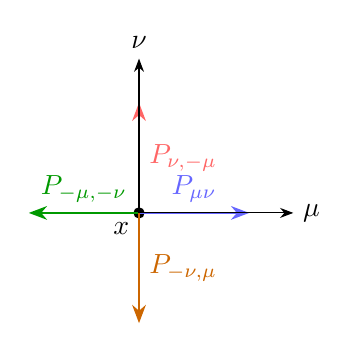
\begin{tikzpicture}[scale=1.4, >=Stealth]
  \filldraw (0,0) circle (1.3pt) node[below left] {$x$};
  \draw[->, thick, blue!60] (0,0) -- (1,0) node[midway, above] {$P_{\mu\nu}$};
  \draw[->, thick, red!60] (0,0) -- (0,1) node[midway, right] {$P_{\nu,-\mu}$};
  \draw[->, thick, green!60!black] (0,0) -- (-1,0) node[midway, above] {$P_{-\mu,-\nu}$};
  \draw[->, thick, orange!80!black] (0,0) -- (0,-1) node[midway, right] {$P_{-\nu,\mu}$};
  \draw[->] (0,0) -- (1.4,0) node[right] {$\mu$};
  \draw[->] (0,0) -- (0,1.4) node[above] {$\nu$};
\end{tikzpicture}
\end{center}

参考约定下流化场强为
\begin{equation}\label{eq:clover_F}
F_{\mu\nu}(x) = -\frac{i}{8}
\Bigl( Q_{\mu\nu}(x) - Q_{\mu\nu}^{\dagger}(x) \Bigr)
\end{equation}
（代码取 $a=1$、$g_0=1$ 的格点归一化。）该对象是有限格距的色矩阵：由于
四叶和与高阶格距项，未投影时可以含有单位阵分量。

\subsubsection{无迹（traceless）生产投影}

生产投影为
\begin{equation}\label{eq:traceless}
F_{\mu\nu}^{\rm tl} = F_{\mu\nu} - \frac{\tr F_{\mu\nu}}{N_c}\mathbf 1,
\qquad F_{\nu\mu}=-F_{\mu\nu}
\end{equation}
\code{gradient\_flow\_gluon\_ope} 同时保存 \code{legacy\_untraced} 与
\code{traceless} 两种 field projection，但只把后者作为 production
selector；两者的差异是有限格距离散差异，不能在分析中静默混用。Clover
场强的天然 $\order{a^2}$ 改进性质来自：(1) 四个 plaquette 的反对称组合
消除了单个 plaquette 的 $\order{a}$ 误差；(2) 取反厄米部分消除色单态
贡献；(3) 四方向对称平均部分恢复 Lorentz 协变性。

\subsection{对偶场强张量}

对偶场强张量 $\Ftmunu$ 通过 Levi-Civita 张量与 $F$ 联系：
\begin{equation}\label{eq:dual_F}
\Ftmunu = \frac{1}{2}\,\eps_{\mu\nu\rho\sigma}\,F^{\rho\sigma}
\end{equation}
其中 $\eps_{\mu\nu\rho\sigma}$ 是四维完全反对称张量，Euclidean 约定
$\eps_{xyzt}=+1$（代码坐标顺序 $(x,y,z,t)=(0,1,2,3)$）。实现上按
Einstein 求和对 $(\rho,\sigma)$ 逐分量缩并
（$\tilde F_{\mu\nu}=\frac12\sum_{\rho,\sigma}\eps_{\mu\nu\rho\sigma}
F_{\rho\sigma}$，\code{compute\_dual\_field\_strength}）：
\begin{equation}
\tilde F_{tx} = \eps_{txyz}\,F_{yz}, \qquad
\tilde F_{ty} = \eps_{tyzx}\,F_{zx}, \qquad
\tilde F_{tz} = \eps_{tzxy}\,F_{xy},
\end{equation}
以及空间三分量
$\tilde F_{xy}=\eps_{xyzt}F_{zt}$、$\tilde F_{xz}=\eps_{xzty}F_{ty}$、
$\tilde F_{yz}=\eps_{yztx}F_{tx}$（每对由「其余两个指标」的唯一场强给出
，这正是 Euclidean 对偶把时-电分量与空-磁分量互换的结构）。代码只存六个
canonical Lorentz pair，反向请求通过反对称性取负
（canonical pair 缓存 + 符号取反）——避免重复计算
Clover，并使 $F_{\mu\nu}$ 与 $\Ftmunu$ 的轴顺序明确。场强字典
\code{compute\_dual\_field\_strength} 与场强字典
\code{\_field\_dictionary} 对每个投影构造
\begin{equation}
\mathcal{F} = \bigl\{\,F_{\mu\nu}\;:\;(\mu,\nu)\in
\{(0,1),(0,2),(0,3),(1,2),(1,3),(2,3)\}\,\bigr\},
\qquad F_{\nu\mu} = -F_{\mu\nu},
\end{equation}
即只保存 $\mu<\nu$ 的六个独立分量（全部 $4\times4=16$ 个有序对由反对
称性给出）；请求 $(\mu,\nu)$ 时按 $\nu-\mu$ 的符号返回对应的 canonical
分量（$\mu>\nu$ 时取负）。
\textbf{无迹投影}按式~\eqref{eq:traceless} 施加于每个分量；两个投影
（legacy\_untraced / traceless）共用同一批 plaquette 计算，差异仅为
$\frac{\tr F}{3}\mathbf 1$ 的单位阵扣除，因此可同时输出而几乎不增加
计算量。

\subsection{直线 Wilson 线与规范不变性}
\label{sec:wilson-line}

连接 $0$ 和 $z\hat z$ 的 Wilson 线是路径有序指数的离散化——格点上为
规范链接乘积。schema-v2 参考约定沿 $z_{\rm dir}=2$ 保存\textbf{原始正负
两方向}：
\begin{align}
M_{\mu\lambda;\nu\rho}^{+}(z)
&=\sum_{\boldsymbol x}
\Tr\!\left[
F_{\mu\lambda}(x+z\hat z)\,W^\dagger(x+z,x)\,
F_{\nu\rho}(x)\,W(x,x+z)
\right], \label{eq:bilocal-plus}\\
M_{\mu\lambda;\nu\rho}^{-}(z)
&=\sum_{\boldsymbol x}
\Tr\!\left[
F_{\mu\lambda}(x-z\hat z)\,W(x-z,x)\,
F_{\nu\rho}(x)\,W^\dagger(x,x-z)
\right]. \label{eq:bilocal-minus}
\end{align}
在 $z=0$ 两式退化为同一个局域矩阵乘积：
\begin{equation}
M^+(0)=M^-(0), \qquad
M_{\rm odd}(0)=M^+(0)-M^-(0)=0
\end{equation}
——这一几何恒等式是 OPE 验证器（\code{validate\_gradient\_flow\_gluon\_ope}
）的强检验之一。

规范变换下
\begin{equation}
F(x)\mapsto G(x)F(x)G^\dagger(x), \qquad
W(x,x+z)\mapsto G(x)\,W(x,x+z)\,G^\dagger(x+z)
\end{equation}
代入式~\eqref{eq:bilocal-plus} 后，端点的 $G$ 与 $G^\dagger$ 在 trace 中
相消，所以\textbf{完整空间和是规范不变的}。契约测试
\code{test\_straight\_wilson\_line\_full\_sum\_is\_gauge\_invariant} 在随机
局域规范变换下实测全 OPE 不变（约 $2.1\times10^{-16}$）。只在某个点比较
矩阵元素、或把两端场强放在不同的链接几何上而没有 Wilson 线，都会破坏
这个论证。

\paragraph{五步构造法的公式化}对固定 $(\mu,\lambda;\nu,\rho)$ 与
$z$，格点实现的五步构造（连续理论到离散的逐段翻译）：
\begin{enumerate}
  \item \textbf{平移}：把第一端点场强放到 $z$ 位置
  （$F_{\mu\lambda}(x+z\hat z)$，格点上为整场 \code{roll}）；
  \item \textbf{反向线}：从 $z$ 走到 $0$，逐段共轭链接乘积
  \begin{equation}
  W^\dagger(x+z,x) = \prod_{k=z/a-1}^{0} U_z^\dagger(x+k\hat z),
  \end{equation}
  \item \textbf{插入}：在 $0$ 处乘第二端点场强（$F_{\nu\rho}(x)$ 或
  对偶 $\widetilde F_{\nu\rho}(x)$）；
  \item \textbf{正向线}：从 $0$ 走回 $z$，
  \begin{equation}
  W(x,x+z) = \prod_{k=0}^{z/a-1} U_z(x+k\hat z),
  \end{equation}
  \item \textbf{收缩}：取色迹 $\trc[\cdots]$ 并对空间点求和
  $\sum_{\boldsymbol x}$（所有乘法为批量 $3\times3$ 复矩阵乘）。
\end{enumerate}
五步的次序不可交换（路径排序 $\mathcal P$ 的离散语义）；负方向
（$-z$）用同一构造但把平移与线的方向反转——两个原始方向的同时保存
正是 even/odd 恒等式检验的几何前提。

\subsection{六个 OPE 组件与非极化/螺旋度算符}
\label{sec:unpol-hel}

令 Wilson 线沿 $z$，横向方向为 $i,j\in\{x,y\}$，Euclidean 时间方向为
$t=3$。定义三个 primitive：
\begin{equation}
T_i = M_{ti;ti}, \qquad T_j = M_{tj;tj}, \qquad S_0 = M_{ij;ij}
\end{equation}
schema-v2 保存的六组件为
\begin{equation}\label{eq:components}
\code{ti}=T_i,\quad \code{tj}=T_j,\quad \code{ij\_single}=S_0,\quad
\code{Mtiti}=T_i+T_j,\quad \code{Mijij}=2S_0,\quad \code{combined}
\end{equation}
因此 \code{Mtiti} 与 \code{Mijij} 是可由 primitive 逐点重构的独立诊断
（$z=0$ 处 $T$、$S$ 相等，这是 odd 组合在 $z=0$ 恒为零的代数原因）。

\subsubsection{非极化通道}

Minkowski 伪分布结构 $\mathcal O_U^{\mathrm M}
=\sum_{i=x,y}M^{\mathrm M}_{0i;i0}+2M^{\mathrm M}_{xy;yx}$ 经 Wick 词典
$M^{\mathrm M}_{0i;i0}=U^E_{ti}$、$2M^{\mathrm M}_{xy;yx}=-2U^E_{xy}$ 变为
\begin{equation}\label{eq:unpol-combination}
\boxed{\;O_U^{\rm GF}(z) = T_U^{\rm GF}(z)-S_U^{\rm GF}(z)\;},
\qquad
T_U=U^E_{tx}+U^E_{ty},\quad S_U=2U^E_{xy}
\end{equation}
即代码分量的
\begin{equation}
O_U = M_{tx;tx}+M_{ty;ty}-2M_{xy;xy} = \code{Mtiti}-\code{Mijij}
\end{equation}
（arXiv:2510.26425v2 的 Euclidean 指标版本）。物理非极化投影取
\textbf{even} 分离：
\begin{equation}\label{eq:even-odd}
O_{U,\rm even} = O_U(+z) + O_U(-z),
\end{equation}
这是生产 selector
\code{(channel=unpolarized, orientation=even\_sum,
component=combined, projection=Re)}。

\subsubsection{螺旋度通道}

Minkowski 螺旋度张量双局域取
$\mathcal O_{\Delta g}^{\rm M}=\sum_{i=x,y}\widetilde M^{\rm M}_{0i;0i}
+2\widetilde M^{\rm M}_{xy;xy}$（第二个场强做对偶）。由电-磁分解
$E_i=F^{\mathrm M}_{0i}$、$F^{\mathrm M}_{ij}=-\eps_{ijk}B_k$，目标结构为
$E_xB_x+E_yB_y-2B_zE_z$；逐项 Wick 转动（利用式~\eqref{eq:wick-dictionary}）
给出 $\widetilde M^{\rm M}_{0i;0i}=+iH^E_{ti}$、
$2\widetilde M^{\rm M}_{xy;xy}=-2iH^E_{xy}$，去掉共同的 $i$ 后，代码基底
中的理论目标为
\begin{equation}\label{eq:hel-physical}
\boxed{\;O_H^{\rm GF}(z)=T_H^{\rm GF}(z)-S_H^{\rm GF}(z)\;},
\qquad
T_H=H^E_{tx}+H^E_{ty},\quad S_H=2H^E_{xy}
\end{equation}
螺旋度的自旋相关部分取 \textbf{odd} 分离：
$O_{H,\rm odd}=O_H(+z)-O_H(-z)$（arXiv:2207.08733v2 的 odd-in-$z$ 目标）。

\textbf{存储约定与理论目标的关键区分}：参考生产数组在 helicity 通道的
\code{combined} 保存的是
\begin{equation}
O_H^{\rm stored} = \code{Mtiti}+\code{Mijij} = (T_H+S_H)
\end{equation}
它保留作诊断；物理 helicity 目标由 selector
$(T_H-S_H)_{\rm odd}$ 得到（\code{physical\_helicity\_ratio} 的
\code{orientation} selector）。把保存约定的加号直接称为
唯一物理 helicity 定义，会把诊断和目标混淆——参考 README 的三个诊断
$(T_H-S_H)_{\rm odd}$、$(T_H+S_H)_{\rm odd}$、$(T_H)_{\rm odd}$ 中只有
第一个由 Wick 转动与 $(E\text{-}B)$ 结构确定为 production target。

\subsubsection{方向投影不引入 $1/2$}

\begin{equation}
O_{\rm even} = O_{+z}+O_{-z}, \qquad
O_{\rm odd} = O_{+z}-O_{-z}
\end{equation}
（数组不除以 2。）验证器同时检查方向线性关系、$z=0$ odd 零值与六组件
组合恒等式（\code{test\_six\_component\_identities\_and\_helicity\_selector}
）。

\subsection{TMD staple 算符与可乘可重整组合}
\label{sec:tmd-operator}

\subsubsection{伴随表示的准 TMD 算符}

TMD 通道在共线直线 Wilson 线的基础上引入横向位移 $\bperp$。伴随表示下
的胶子准 TMD 算符为
\begin{equation}\label{eq:M-adj-tmd}
M^{\mu\lambda;\nu\rho}(z,\bperp)
= F^{\mu\lambda}(z\hat z+\bperp)\cdot U_{\mathrm{adj}}(\text{staple})
\cdot F^{\nu\rho}(0)
\end{equation}
其中 \textbf{staple Wilson 线} $W_\sqsubset(z,\bperp)$ 的「纵向臂 + 横向
翼 + 纵向臂」三段路径为基础表示格点实现：
\begin{equation}\label{eq:staple-wilson}
W_\sqsubset = U_z^\dagger\bigl((z+L)\hat z+\bperp,\;\bperp\bigr)
\cdot U_\perp\bigl((z+L)\hat z+\bperp,\;(z+L)\hat z\bigr)
\cdot U_z\bigl((z+L)\hat z,\; z\hat z\bigr)
\end{equation}
即
$M(\boldsymbol x)=\trc[\,F(\boldsymbol x)\,W_\sqsubset(\boldsymbol x,
\boldsymbol y)\,F(\boldsymbol y)\,W_\sqsubset^\dagger(\boldsymbol x,
\boldsymbol y)\,]$，
$\boldsymbol y=\boldsymbol x+z\hat z+\bperp$
（\code{pyqcd/renorm/\_tmd.py} 的 \code{staple\_wilson\_line}；纵向/横向
空间方向经 \code{\_validate\_spatial\_directions} 校验，$\bperp\to0$
极限约化为直线 Wilson 线共线算符）。

\paragraph{staple 几何的约束}三段路径的几何约束与自由度：
\begin{itemize}
  \item \textbf{方向约束}：纵向 $z_{\rm dir}$ 与横向翼方向 $b_{\rm dir}$
  必须为不同的空间方向（$0=x,1=y,2=z$；违例直接拒绝）——这排除了路径
  自交与零臂长的退化情形；
  \item \textbf{臂长}：翼长默认取 $L=z$（与纵向分离同量级），保持
  staple 的「 $\sqsubset$ 形」对称；臂长是\textbf{方案参数}而非物理
  输入，跨组态保持一致并在 metadata 登记；
  \item \textbf{周期边界}：三段路径各段长度均须 $<L/2$（空间周期下
  不绕边界；绕边界的 staple 需要显式边界符号语义，本库不启用）；
  \item \textbf{规范不变性}：三段路径闭合于两端场强之间，规范变换的
  $G(x)$/$G^\dagger(y)$ 在两端 trace 相消——与直线情形
  （式~\eqref{eq:bilocal-plus}）同一论证；
  \item \textbf{共线极限}：$\bperp\to0$ 时翼段消失、两纵向臂方向相同，
  $W_\sqsubset\to\mathbf1$ 的平移补丁 + 直线 Wilson 线，算符约化为
  共线通道——这保证 TMD 与共线 PDF 共享同一套 even/odd、组件与统计
  层（只多出 $\bperp$ 依赖）。
\end{itemize}

\subsubsection{乘性可重整的 Lorentz 组合}

令 $i,j$ 为 $z_{\rm dir}$ 之外的两个空间方向，可乘性重整化组合为
\begin{equation}\label{eq:O-mult-tmd}
\boxed{\;O(z,\bperp) = M^{ti;ti} + M^{tj;tj} - 2\,M^{ij;ij}\;}
\end{equation}
该组合的一圈 UV 反常量纲使整体（至少一圈水平）\textbf{乘法可重整化}——
Li、Ma 和 Qiu（2018，arXiv:1809.01836）证明了所有独立准胶子算符在规范
不变 UV 正规化下无混合可乘重整；组合式~\eqref{eq:O-mult-tmd} 的关键在于
各分量的 UV 幂次发散在组合内相消，线性发散归入 Wilson 线自能（第
\ref{sec:renorm} 章）。这与旧文档的 Eq.~(25) 锚点完全对应：
\begin{equation}
O_{\text{unpol}}(z) = \sum_{\mu\ne z}\sum_{\nu\ne z} g^{\mu\nu}
F_{z\mu}(z)\,W(z,0)\,\tilde{F}_{\nu}^{\;z}(0)
\end{equation}

\subsubsection{不变振幅与 TMD-PDF 的关系}

双局域矩阵元的不变振幅分解给出
\begin{equation}\label{eq:Mpp-PDF}
-M_{pp}(\nu,\bperp) = \frac12\int_{-1}^{1}\mathrm{d}x\,
e^{-ix\nu}\,x\,g(x,\bperp),
\qquad
M^{ti;it}+M^{ji;ij} = 2p_0^2 M_{pp}(\nu,\bperp)
\end{equation}
（\code{\_tmd.py} 的 \code{Mpp\_extract/PDF} 语义；$\nu=zP_z$ 为 Ioffe
时间。）

\subsection{Symanzik 改进与涂抹方案对比}

\subsubsection{Symanzik 有效作用量视角}

格点理论可视为连续理论的有效理论，其作用量包含被格距幂次压低的高维算符：
\begin{equation}
S_{\text{eff}} = S_{\text{cont}} + a^2 \int \mathrm{d}^4 x \,
c_2\,\mathcal{O}_6(x) + a^4 \int \mathrm{d}^4 x \,
c_4\,\mathcal{O}_8(x) + \cdots
\end{equation}
其中 $\mathcal{O}_{2k}$ 是量纲为 $2k$ 的定域算符。对于 Wilson 胶子作用量
（仅 $1\times1$ plaquette），前导误差为 $\order{a^2}$；在作用量中纳入
$1\times2$ 矩形圈（L\"uscher-Weisz 改进作用量）可在经典水平消除
$\order{a^2}$ 项。对含 Wilson 线的\textbf{非定域}算符，Symanzik 分析的
结论是：使用四叶 Clover 场强后场强端点的前导离散化误差为 $\order{a^2}$；
但离散 Wilson 线本身可能引入额外的 $\order{a}$ 效应——这需要涂抹或梯度
流来缓解（HYP 涂抹后误差结构回到 $\order{a^2}$ 主导；梯度流方案中
$r_{\rm flow}\gg a$ 时链接的离散化细节被平滑，等效地压制了 $\order{a}$
项）。

\subsubsection{Tadpole（平均场）改进}

在格点微扰论中，规范链接的高阶 tadpole 图贡献大的、纯规范的重整化因子
。Lepage--Mackenzie 的 tadpole 改进通过重新标度链接变量
$U_\mu \to U_\mu/u_0$ 吸收这些贡献，其中 $u_0$ 由 plaquette 平均估计：
\begin{equation}
u_0 = \left( \frac{1}{3}
\bigl\langle \operatorname{Re}\operatorname{Tr} P_{\mu\nu} \bigr\rangle
\right)^{1/4},
\end{equation}
在裸耦合下 $\frac13\langle\operatorname{Re}\operatorname{Tr}P\rangle
=1-\frac{g_0^2}{12}\sum_{\mu<\nu}\cdots$（一阶展开），因此
$u_0<1$、$1/u_0>1$——把被「拉长」的链接还原到树图值。本库代码取
$a=1,g_0=1$（归一化已吸收），但跨格距的绝对归一化必须对齐——参考实现
侧把该因子记为 tree-level 归一化
$(gF)_{\rm cont}=\kappa_F(a,\tau)\,F_{\rm code}$，双局域需乘
$\kappa_F^2$；GF-to-$\MSbarM$ 系数在 field normalization 未对齐前不能
直接套用（第 \ref{sec:matching} 章）。

\subsubsection{HYP 涂抹的三步过程}

\textbf{HYP（Hypercubic）涂抹}（Hasenbusch 2001）在一个超立方体内分
三步进行，每一步只对特定方向的链接做 staple 平均并投影回 SU(3)：
\textbf{第一步}在垂直于方向 $\mu$ 的超立方体内部面上涂抹（仅涉及与
$\mu$ 正交的方向），
\begin{equation}
\bar U_\mu^{(1)}(x) = \mathcal P_{\mathrm{SU(3)}}\!\left[
(1-\alpha_1)U_\mu(x) + \frac{\alpha_1}{2}
\sum_{\nu\ne\mu} \bigl(\text{$\nu$ 方向的内部 staple}\bigr) \right],
\end{equation}
\textbf{第二步}在包含 $\mu$ 与另一方向的三维子集内对第一步的结果进一步
涂抹，\textbf{第三步}将涂抹限制在完全位于超立方体内的链接上。投影
$\mathcal P_{\mathrm{SU(3)}}$ 取使
$\operatorname{Re}\operatorname{Tr}[V^\dagger\bar U]$ 极大化的
$V\in\mathrm{SU}(3)$（极值条件 $V\bar U=\bar U V\bar U^\dagger$ 为
厄米矩阵，由 SVD 求解——本库 stab0\_2 已把批量 eigh bug 修复为 SVD）。
标准参数为 $\alpha_1=0.75$、$\alpha_2=0.6$、$\alpha_3=0.3$。涂抹后
Wilson 线的线性发散系数 $\delta m$ 显著减小、信噪比改善，且连续极限下
与未涂抹算符同属同一普适类。本库 HYP 实现（SU(3) 精度 $10^{-16}$，
stab0\_2 验证）对规范链接的预处理显著改善胶子 OPE 算符在中等与较长
Wilson 线（$z\gtrsim5a$）的信号质量。

\subsubsection{HYP 与梯度流的分工及两路径隔离}

\begin{center}
\small
\begin{tabular}{c c c c}
\toprule
\textbf{路径} & \textbf{预处理} & \textbf{算符层次} & \textbf{用途} \\
\midrule
legacy/TMD 路径 & HYP/stout 可选 & staple/TMD、$Z_R$、混合、NLO & docker 基线 + TMD 主链 \\
schema-v2 路径 & 薄链接 + 四维 flow & 直线六组件 + ratio-v2 & 参考复现与交叉校验 \\
\bottomrule
\end{tabular}
\end{center}
两层的语义由 metadata（\code{input\_scheme}、\code{schema}、\code{status}
）显式记录，\textbf{不互称、不静默混用}：把 legacy 有限格距未去迹 OPE
当作生产 traceless OPE、把现有 TMD staple 路径当作参考直线 OPE，都是
20260909 审计报告明确登记的风险偏差。三种平滑手段的对照：

\begin{center}
\small
\begin{tabular}{c c c}
\toprule
\textbf{手段} & \textbf{平滑尺度} & \textbf{重整化语义} \\
\midrule
HYP & 定域（超立方体内，$\sim a$） & 无（保持裸算符方案） \\
Stout & 定域（nstep 与 $\rho$ 控制） & 无（同上） \\
四维 Wilson flow & $\sqrt{8\tau}$（流时间扫描） & \textbf{有}（$\tau$ 即重整化方案入口） \\
\bottomrule
\end{tabular}
\end{center}
Stout 涂抹（nstep=20、$\rho=0.12$ 对齐真实系综，
\code{pyqcd/smear/\_stout.py}）作为涂抹备选方案保留；四维 flow 的
关键差别在于它\textbf{自带重整化方案}（SFTE，第 \ref{sec:renorm} 章）。

\paragraph{涂抹方案的数值事实}本库的对照数值记录：HYP 涂抹（SU(3)
精度 $10^{-16}$、平滑化、stab0\_2 修复批量 eigh）与四维 flow 在同一
组态上的定性一致（相关系数 $r=0.965$，stab0\_4）——两类平滑在
$\order{a}$ 尺度上给出一致的链接平滑；stout（nstep=20、$\rho=0.12$）
经 cmp1 对照定位其根因（插桩证据：视图去迹生效、布局依赖生产栈，
test10\_6\_1），S10 定性结论为「pyqcd 物理正确」（test10\_7\_1）。
这些事实说明：**平滑手段的选择不影响物理结论，但改变有限格距的
离散误差结构**——因此在跨格距比较前，各格距必须统一平滑方案（或
在匹配系数中显式计入差异）。

\subsection{边界条件与有限体积}

格点 QCD 使用（反）周期性边界条件：
\begin{equation}
U_\mu(x+L_\nu\hat\nu)=U_\mu(x)\;\;\forall\,\mu,\nu\;(\text{规范场周期}),
\qquad \psi(x+N_t\hat t)=-\psi(x)\;(\text{费米子时间方向反周期}),
\end{equation}
这给出有限温度关系 $T=1/(aN_t)$。Wilson 线的长度受空间周期边界限制：
实际可用的最大长度为 $z_{\max}\le L/2$——超过这个长度，正向与反向
Wilson 线在拓扑上不可区分（Hermiticity 与宇称自洽检验也随之变味）。
参考生产 $L=32$ 的 $z/a$ 范围为 $0..24$（$24<32/2$ 合规），物理距离
$24a\approx1.86$ fm（$a=0.0775$ fm）；蒸馏基线 $L=24$ 时
$z/a=0..11$。时间方向上，三点函数的时序关系
$t_{\text{src}}\le t_{\text{op}}\le t_{\text{sink}}$ 在模 $N_t$ 意义下
定义（第 \ref{sec:factorization} 节）。

% ===========================================================================
\section{关联函数分解与 disconnected 通道}
\label{sec:factorization}
% ===========================================================================

\subsection{三点关联函数与 disconnect 图}

\subsubsection{三点关联函数的结构}

胶子 TMD/PDF 的格点计算需要构造包含胶子算符 $\mathcal{O}(z)$（共线直线
或 TMD staple）的核子三点关联函数：
\begin{equation}\label{eq:C3_def}
C_3(t_{\text{sep}}; z, \mathbf{P}) =
\braket{\Omega \big|
\;\mathcal{N}_\alpha(\mathbf{P}, t_{\text{sink}}) \;
\mathcal{O}(z; t_{\text{op}}) \;
\bar{\mathcal{N}}_\beta(\mathbf{P}, t_{\text{src}})
\big| \Omega}
\end{equation}
其中 $t_{\text{sep}} = t_{\text{sink}} - t_{\text{src}}$ 是 source-sink
时间分离；$t_{\text{op}}$ 是算符插入时间；
$\mathcal{N}_\alpha(\mathbf{P}, t) = \sum_{\mathbf{x}}
e^{-i\mathbf{P}\cdot\mathbf{x}} \mathcal{N}_\alpha(\mathbf{x}, t)$ 是动量
投影的质子插值算符；$\mathcal{O}(z) = \sum_{\mathbf{y}}
\mathcal{O}(\mathbf{y}, z)$ 是空间平均后的胶子算符（零动量插入）；
$\alpha,\beta$ 是 Dirac 旋量指标。

\subsubsection{Wick 收缩的分类：Connected 与 Disconnected}

对式~\eqref{eq:C3_def} 中的夸克场做 Wick 收缩，得到两类拓扑不同的图。

\textbf{类型 A：Connected 图}——胶子算符中的规范场通过夸克-胶子顶点与
核子中的夸克线相连，需对每个组态计算带 $F_{\mu\nu}$ 插入的 sequential
source 传播子。\textbf{类型 B：Disconnected 图}——胶子算符的规范场与
核子中所有夸克线没有直接 Wick 收缩，夸克部分与胶子部分完全分离：
\begin{equation}\label{eq:disconnected}
C_3^{\text{disc}} = \big\langle\;
\tr\big[ S_u \Gamma S_d \Gamma S_u \big]_{\text{quark}}
\;\times\;
\trc\big[ F_{z\mu}(z) \, W(z,0) \, \tilde{F}^{\mu z}(0) \big]_{\text{gluon}}
\;\big\rangle_{\text{gauge}}
\end{equation}
夸克部分和胶子部分仅通过规范组态的整体平均关联。

\subsubsection{为什么胶子算符只有 disconnected 图}

从量子场论的角度，这个结论有三层依据：

\begin{enumerate}
  \item \textbf{算符的组成}：$\mathcal O(z,\bperp)
  =\trc[F_{\mu\lambda}\,W\,F_{\nu\rho}\,W^\dagger]$ 仅包含规范场
  $A_\mu^a$ 及其泛函，不含任何夸克场 $\psi,\bar\psi$；
  \item \textbf{Grassmann 积分的因子化}：三点关联函数的路径积分表示为
  \begin{equation}
  C_3 = \frac{1}{Z} \int \mathcal{D}U \mathcal{D}\psi \mathcal{D}\bar\psi
  \; e^{-S_G[U]-\bar\psi D[U]\psi} \;
  (\mathcal{N}\bar{\mathcal{N}})[U,\psi,\bar\psi]\;
  \mathcal{O}(z,\bperp)[U],
  \end{equation}
  由于 $\mathcal O$ 与夸克场对易，对夸克场积分后它作为纯 $U$ 的函数
  提出积分号外：
  \begin{equation}
  C_3 = \frac{1}{Z} \int \mathcal{D}U \; e^{-S_G[U]} \; \det(D[U]) \;
  \underbrace{\big[\text{Wick 收缩的 } \mathcal{N}\bar{\mathcal{N}}
  \big]_{\text{夸克部分}}}_{\equiv\; C_2[U]}
  \;\underbrace{\mathcal{O}(z,\bperp)[U]}_{\text{胶子部分}}
  \label{eq:grassmann-factorization}
  \end{equation}
  \item \textbf{connected 消失的条件}：若胶子算符经夸克-胶子顶点
  $g_0\bar\psi\gamma^\mu A_\mu\psi$ 与夸克线耦合，需要 $F_{\mu\nu}$ 中
  的规范链接与夸克传播子共享量子涨落；但 $\mathcal O(z,\bperp)$ 是
  \textbf{规范不变的整体算符}（场强由 clover 定义、Wilson 线保证规范
  不变性），其 Wick 收缩在 leading order 不能与夸克线连接——任何此类
  连接都要求至少一个胶子从夸克线辐射出去，是 $\order{g_0}$（微扰）或
  完全非微扰框架下的次级拓扑。
\end{enumerate}
结论：在 leading order，胶子 quasi-PDF/TMD 的三点关联函数仅包含
disconnected 贡献（Fan et al.\ 2018；Alexandrou et al.\ 2021 已在格点
上显式检验 connected 贡献在统计误差内与零一致；压低机制与色因子
$\sim1/N_c$ 相关——软胶子交换需要胶子带有与夸克动量可比拟的横向动量，
且矢量耦合的色结构自然压低该贡献）。

\begin{figure}[htbp]
\centering
\begin{tikzpicture}[scale=1.0, >=Stealth,
  quark/.style={very thick, blue!70!black},
  gluon/.style={very thick, red!60!black},
  vertex/.style={fill=black, circle, inner sep=1.2pt},
  lbl/.style={font=\footnotesize}
]
  \node[lbl, above] at (0,3.4) {\textbf{(a) Connected}};
  \draw[quark] (0,0) -- (0.8,1.2) -- (2.0,1.8) -- (3.2,1.2) -- (4.0,0);
  \draw[quark] (0,3) -- (0.8,1.8) -- (2.0,1.2) -- (3.2,1.8) -- (4.0,3);
  \draw[quark] (0,1.5) -- (4.0,1.5);
  \draw[gluon] (2.0,1.5) -- (2.0,3.0);
  \node[lbl, red!60!black] at (2.5,2.7) {$O(z,\bperp)$};
  \filldraw[vertex] (0.8,1.8) circle (1.5pt);
  \filldraw[vertex] (2.0,1.8) circle (1.5pt);
  \filldraw[vertex] (2.0,1.2) circle (1.5pt);
  \filldraw[red!60!black] (2.0,1.5) circle (2.5pt);
  \node[lbl] at (4.5,0)   {$N(t_{\text{sink}})$};
  \node[lbl] at (4.5,3)   {$\bar{N}(t_{\text{src}})$};
  \begin{scope}[xshift=7.6cm]
    \node[lbl, above] at (0,3.4) {\textbf{(b) Disconnected}};
    \draw[quark] (0,2.0) -- (0.8,2.8) -- (1.6,2.4) -- (2.4,2.8) -- (3.2,2.0);
    \draw[quark] (0,3.0) -- (0.8,2.2) -- (1.6,2.6) -- (2.4,2.2) -- (3.2,3.0);
    \draw[quark] (0,2.5) -- (3.2,2.5);
    \node[lbl] at (3.7,2.0) {$N$};
    \node[lbl] at (3.7,3.0) {$\bar{N}$};
    \node[lbl, blue!70!black] at (1.6,1.7) {核子 2pt: $C_2(\Delta t,\mathbf P)$};
    \draw[dashed, gray] (-0.8,1.2) -- (4.2,1.2);
    \node[lbl, gray] at (5.0,1.2) {（仅经 $\langle\cdot\rangle_{\text{gauge}}$ 关联）};
    \draw[gluon] (0.4,0.8) -- (0.4,0);
    \draw[gluon] (1.2,0.8) -- (1.2,0);
    \draw[gluon] (2.0,0.8) -- (2.0,0);
    \draw[gluon] (2.8,0.8) -- (2.8,0);
    \draw[gluon, loosely dotted] (0.4,0.8) -- (2.8,0.8);
    \node[lbl, red!60!black, fill=white] at (0.25,0.6) {$F(z)$};
    \node[lbl, red!60!black, fill=white] at (2.95,0.6) {$\tilde F(0)$};
    \node[lbl, red!60!black] at (1.6,-0.5) {纯规范场 OPE:
    $\langle O(z,\bperp)\rangle_{\text{gauge}}$};
  \end{scope}
\end{tikzpicture}
\caption{三点关联函数的两种 Wick 收缩拓扑。\textbf{(a)} Connected：胶子
算符经夸克-胶子顶点与核子夸克线耦合。\textbf{(b)} Disconnected：夸克部分
（核子传播子）与胶子部分（OPE 算符）拓扑分离，仅通过同一规范组态平均
关联。对胶子准 TMD/PDF 算符，只有 disconnected 图有贡献。}
\label{fig:connected_vs_disconnected}
\end{figure}

\subsection{因子化：三点函数到两点函数与 OPE 的解耦}

基于 disconnected 拓扑，三点关联函数可以写为逐组态的乘积：
\begin{equation}\label{eq:factorization_exact}
C_3(t_{\text{sep}}; z, \mathbf{P}) =
\frac{1}{N_{\text{conf}}} \sum_{\text{conf}}
\underbrace{C_2(t_{\text{sep}}; \mathbf{P})\big|_{U}}_{\text{核子 2pt}}
\;\cdot\;
\underbrace{O(z,\bperp)\big|_{U}}_{\text{OPE}}
\end{equation}
由于 $C_2[U]$ 的统计涨落已通过蒸馏大幅压制，而 $O(z)[U]$ 的涨落是主要
噪声来源，实际计算采用\textbf{部分因子化}（真空扣除）策略：
\begin{equation}\label{eq:factorization}
\boxed{\;C_3(t_{\text{sep}}; z, \mathbf{P}) \approx
\vev{ C_2(t_{\text{sep}}; \mathbf{P}) }_{\text{conf}} \cdot
\vev{ O(z,\bperp) }_{\text{conf}}
-\operatorname{Cov}_{\text{conf}}(C_2, O)\;}
\end{equation}
更精确地说，ratio-v2 统计层使用的是\textbf{逐组态协方差扣除}（第
\ref{sec:statistics} 章的式~\eqref{eq:c3-cov}）：disconnected 矩阵元由
$\langle O\,C_2\rangle_{\text{conf}}-\langle O\rangle\langle C_2\rangle$
给出，而非简单的均值乘积——这是真空扣除的协方差形式。因子化的数值
条件（协方差足够小、$t_{\text{sep}}$ 足够大使基态饱和、蒸馏截断足够大）
与旧版一致。

\subsubsection{时间结构与边界条件}

三点关联函数中算符的时序为 $t_{\text{src}} \le t_{\text{op}} \le
t_{\text{sink}}$，时间指标在模 $N_t$ 意义下定义：
\begin{equation}
\Delta t \equiv (t_{\text{sink}} - t_{\text{src}}) \bmod N_t, \qquad
\Delta t_{\text{op}} \equiv (t_{\text{op}} - t_{\text{src}}) \bmod N_t
\end{equation}
关联函数按时间分离的谱参数化（含反向传播）已在上一小节给出。对 OPE
期望值的\textbf{时间平均}性质：由于取空间平均后 OPE 在各时间片独立，
\begin{equation}
\vev{O(z)}_{\text{gauge}}
= \frac{1}{N_t}\sum_{t_{\text{op}}=0}^{N_t-1}\sum_{\mathbf{x}}
O(\mathbf x, z; t_{\text{op}})
\end{equation}
\textbf{注}：实际计算对\textbf{所有}时间片 $t_{\text{op}}$ 求平均（而非
仅在 $t_{\text{src}}$--$t_{\text{sink}}$ 之间）可以最大化统计量——
胶子算符不含夸克场，即使 $t_{\text{op}}$ 在窗口之外，quark-disconnected
拓扑也不受影响。这一性质显著提升信噪比。但 ratio-v2 的物理有效性区间
受\textbf{插值时间}约束：
\begin{equation}
O(t_{\text{src}}+\tau_{\rm ins})
= \operatorname{take}\bigl[\,O,\,(t_{\text{src}}+\tau_{\rm ins})
\bmod N_t\,\bigr],
\qquad \text{仅 } 0\le\tau_{\rm ins}\le t_{\rm sep} \text{ 有效},
\end{equation}
其余位置填 NaN（不是静默填零）并保存 \code{valid\_insertion\_mask}
保存 \code{valid\_insertion\_mask}（第 \ref{sec:statistics} 章）。

\subsection{关联函数的谱分解与基态提取}

\subsubsection{完备本征态插入与反向传播}

两点关联函数的谱分解通过插入完备的哈密顿量本征态集合得到：
\begin{equation}\label{eq:C2_spectral}
C_2(\Delta t, \mathbf{P}) = \sum_n Z_n(\mathbf{P})\,
e^{-E_n(\mathbf{P})\,\Delta t},
\qquad Z_n(\mathbf{P}) = \bra{0}\mathcal N(\mathbf P)\ket n
\end{equation}
在周期性时间格点上，反向传播项（态绕过时间边界反向传播）叠加为：
\begin{equation}
C_2(\Delta t,\mathbf P) = \sum_n Z_n(\mathbf P)
\bigl[e^{-E_n\Delta t} + \sigma_{\mathbf P}\,e^{-E_n(N_t-\Delta t)}
\bigr],
\end{equation}
其中 $\sigma_{\mathbf P}=\pm1$ 取决于通道在时间反演/宇称下的符号
（pp 通道 $t_{\rm sink}<t_{\rm src}$ 时符号翻转，见第
\ref{sec:distillation} 章边界符号）。在大 $\Delta t$ 极限下基态主导：
\begin{equation}
C_2 \xrightarrow{\Delta t\to\infty} Z_0(\mathbf P)\,
e^{-E_0(\mathbf P)\,\Delta t}
\end{equation}

\subsubsection{有效质量与 Plateau 拟合}

有效质量定义为
\begin{equation}
m_{\text{eff}}(\Delta t) = \ln\!\left[
\frac{C_2(\Delta t, \mathbf{P})}{C_2(\Delta t+1, \mathbf{P})} \right]
\xrightarrow{\Delta t\to\infty} E_0(\mathbf P)
\end{equation}
（含反向传播修正的推广形式可取
$m_{\rm eff}=\ln[C_2(\Delta t)+\sigma C_2(N_t-\Delta t)]$ 的比值，本库
实战以窗口切割规避反向污染）。在大 $\Delta t$ 时 $m_{\rm eff}$ 趋于
常数 $E_0(\mathbf{P})$；通过 plateau 拟合——在有效质量平稳区域内做
常数拟合——提取基态能量，拟合质量判据为 $\chi^2/\mathrm{dof}\sim1$。
对于矩阵元提取，有效矩阵元为
\begin{equation}
h^{\text{eff}}(z,P_z;\Delta t) =
\frac{C_3(\Delta t; z, P_z)}{C_2(\Delta t; P_z)}
\xrightarrow{\Delta t\to\infty} h + A\,e^{-\Delta E\,\Delta t}
\end{equation}

\subsubsection{多态拟合、Bayesian 约束与 GEVP}

当信噪比不够好时，需包含激发态的双态拟合
\begin{equation}
C_2(\Delta t) = |Z_0|^2e^{-E_0\Delta t} + |Z_1|^2e^{-E_1\Delta t},
\end{equation}
对应的有效矩阵元形式为 $h^{\rm eff}=h+Ae^{-\Delta E\Delta t}+\cdots$
（$\Delta E=E_1-E_0$）。基态饱和判据：$\Delta t\cdot\Delta E\gtrsim2$
时激发态污染 $<15\%$；对典型核子能隙（$\Delta E\sim0.5$ GeV），
$\Delta t_{\rm sep}\gtrsim1$ fm 时基态占据主导。小 $N$（组态数）、多
参数情形下，传统 $\chi^2$ 拟合不稳定，\textbf{Bayesian 约束拟合}引入
参数先验：
\begin{equation}\label{eq:chi2-aug}
\chi^2_{\text{aug}} = \chi^2 + \sum_k \frac{(p_k-\tilde p_k)^2}
{\sigma_{p_k}^2},
\end{equation}
其中 $\tilde p_k$、$\sigma_{p_k}$ 是先验均值与宽度（可取物理预期，如
$E_1-E_0\sim0.5$ GeV）。比值结构
\begin{equation}
R(T,\tau) = M + A\,e^{-\Delta E\tau}
+ B\,e^{-\Delta E(T-\tau)} + C\,e^{-\Delta E T} + \cdots
\end{equation}
（\pathref{refer/donghx/Gradient_Flow_GluonPDF/physics-conventions.md}
）同时解释了端点切割与 Sumratio 斜率比直接 plateau 更不敏感的原因；
\textbf{多态 Ratio 拟合的可辨识性}不能仅凭优化器收敛判定——
$\Delta E$ 必须来自相容的 $C_2$ 谱分析或使用透明先验并保留先验约束
状态。GEVP 方法系统分离基态与低激发态：
\begin{equation}
C(\Delta t)\,v_n(\Delta t,\Delta t_0)
= \lambda_n(\Delta t,\Delta t_0)\,
C(\Delta t_0)\,v_n(\Delta t,\Delta t_0),
\qquad \lambda_n(\Delta t)\sim e^{-E_n\Delta t},
\end{equation}
其中 $C(\Delta t)$ 是不同插值算符之间的关联函数矩阵（GEVP 对大动量下
核子态的精确提取特别有效；本库 stab13 已修复复数 Hermitian GEVP 的
信息丢失问题并加回归测试）。

对本库 disconnected 通道，由于 OPE 对\textbf{所有}时间片平均（且真空
扣除后比值对 $t_{\text{sep}}$ 的依赖被消除），$h(z,\bperp,P_z)$ 直接从
组态平均后的统计量提取，不需要两步拟合——这是 disconnect 方法的重要
简化。但参考实现仍保留 $t_{\text{sep}}\in[5,15]$ 扫描与端点切割作为
激发态控制诊断。

\subsection{ Eq.~(20) 矩阵元与 Eq.~(25) OPE 的锚点}

对照旧文档的两个公式锚点（本版沿用同一编号语义）：
\textbf{Eq.~(20)}——坐标空间矩阵元
$h(z,P_z)\equiv\braket{P|O(z)|P}/\braket{P|P}$，在格点上通过关联函数比
提取（式~\eqref{eq:ratio-def}），disconnect 通道下
$h^{\text{lat}}\approx\vev{O(z)}_{\text{gauge}}$ 修正为协方差形式；
\textbf{Eq.~(25)}——拆分出的 OPE 算符具体形式
$O_{\text{unpol}}(z)=\sum_{\mu\ne z}\sum_{\nu\ne z}g^{\mu\nu}
F_{z\mu}(z)\,W(z,0)\,\tilde F_\nu^{\;z}(0)$。两个锚点在 schema-v2 中的
对应物分别是 ratio-v2 的 \code{combined} 组件与六组件保存
（第 \ref{sec:unpol-hel} 节）。

\subsubsection{Lorentz 分量分类与方向平均}

在有限格距下 Euclidean 旋转对称性 $O(4)$ 破缺为超立方对称性 $H(4)$，
连续理论中由 Lorentz 对称性关联的分量在格点上需独立处理。对 Wilson 线
沿 $z$ 的构型，非极化三个独立分量为：

\begin{center}
\begin{tabular}{c c c c}
\toprule
\textbf{分量} & \textbf{$(\mu,\nu)$ 组合} & \textbf{物理内容} &
\textbf{连续极限贡献} \\
\midrule
电-电 & $(t,x)$、$(t,y)$ & $F_{zt}W\tilde F^{tz}$ & $E_\perp\cdot E_\perp$ 型 \\
磁-磁 & $(x,y)$ & $F_{zx}W\tilde F^{xz}+F_{zy}W\tilde F^{yz}$ & $B_\perp\cdot B_\perp$ 型 \\
组合 & 全部 & $O_U=M_{tx;tx}+M_{ty;ty}-2M_{xy;xy}$ & Lorentz 不变量 \\
\bottomrule
\end{tabular}
\end{center}
由电-磁分解 $E_i=F^{\mathrm M}_{0i}$、$F^{\mathrm M}_{ij}=-\eps_{ijk}B_k$
：电-电项贡献 $E_\perp^2$ 型结构、磁-磁项贡献 $B_\perp^2$ 型结构；
组合 $O_U$ 正是「$E_\perp^2-B_\perp^2$ 型」的 twist-2 投影（经 Wick
词典后即 $M_{tx;tx}+M_{ty;ty}-2M_{xy;xy}$）。在连续极限下所有分量的
贡献合并为所需 Lorentz 不变量；有限格距下通过\textbf{三方向平均}
（$z_{\rm dir}=x,y,z$ 的动量置换，\code{pyqcd/analysis/\_bare\_matrix.py}
的 \code{dir\_momentum}）部分恢复旋转对称性。\textbf{并行实现的两代
方案}：legacy docker 时代按 Lorentz 对分配 MPI rank（三个分量各占
一个 rank，零通信、完美负载均衡、可随极化/固定规范通道自然扩展到更多
rank）；schema-v2 的单组态实现则在同一进程内对全部 $(\mu,\nu)$ 对
批量构造（逐组态 embarrassingly parallel 的组态级并行由元任务调度层
承担，见第 \ref{sec:workflow} 章）。非极化通道取 even 投影后取实部；
螺旋度通道取 odd 投影后经 $\operatorname{Re}[-iR_H]$ 相位投影。

\paragraph{三方向平均与裸矩阵元组装}有限格距下不同 $z_{\rm dir}$ 的
结果略有差异；裸矩阵元的系综组装按\textbf{动量置换}三方向平均：
\begin{equation}\label{eq:three-dir-average}
h^{\rm bare}(z,\bperp,P_z) = \frac13\sum_{d\in\{x,y,z\}}
h^{(d)}\bigl(\Pi_d(z,\bperp,P_z)\bigr),
\end{equation}
其中 $\Pi_d$ 是把 boost/分离/位移按 $d$ 方向重标的置换（\code{
pyqcd/analysis/\_bare\_matrix.py} 的 \code{dir\_momentum}：对 boost
动量沿 $d$、OPE 组合沿同方向的匹配）；三方向的组态级数据在
configuration-aligned 意义下逐组态平均后再入统计层。三方向与单方向的
差是旋转对称性破缺的直接度量（系统误差预算的输入之一）。

% ===========================================================================
\section{Distillation 方法与动量涂抹}
\label{sec:distillation}
% ===========================================================================

\subsection{Distillation 的基本思想}

\textbf{Distillation}（Peardon et al., 2009，arXiv:0905.2160）是一种夸克
场涂抹方法，用于构建高质量的强子插值算符。基本步骤：
\begin{enumerate}
  \item 计算格点 Laplace 算符的低模本征矢量 $v^{(k)}(x)$；
  \item 用截断的本征矢量展开构建 \textbf{perambulator}——夸克传播子的
  子空间投影；
  \item 所有 Wick 收缩在 $N_{\text{ev}} \times N_{\text{ev}}$ 的子空间内
  完成。
\end{enumerate}
夸克传播子的 Distillation 表示：
\begin{equation}\label{eq:distillation}
S(x, y)_{\alpha\beta}^{ab} \approx \sum_{k,l=1}^{N_{\text{ev}}}
v^{(k)}(x) \, \tau^{(kl)}(t) \, v^{(l)\dagger}(y)
\end{equation}
其中 $\tau$ 是 perambulator。优势：复杂的多夸克关联函数变得可行；本征
矢量可在不同算符/动量间复用；自然实现涂抹并压制 UV 涨落。

\subsubsection{规范协变 Laplace 算符与低模物理}

三维规范协变 Laplace 算符为
\begin{equation}\label{eq:laplace}
\Delta^{ab}_{xy}(t) = \sum_{\mu=1}^{3} \Bigl[
\delta_{x+\hat{\mu},y} \, U_\mu^{ab}(x,t) +
\delta_{x-\hat{\mu},y} \, U_\mu^{\dagger, ab}(x-\hat{\mu},t) -
2\delta_{xy}\delta^{ab} \Bigr]
\end{equation}
本征值问题 $\Delta v^{(k)} = \lambda_k v^{(k)}$，$\lambda_k \ge 0$。
数值求解用 Lanczos 型迭代（大稀疏厄米特征问题）；本征基的正交性与
完备性须验证（本库 V1--V4 压缩与噪声/GS/正交检查契约）。
\textbf{低模的物理意义}：$\lambda_k\sim k^2$（低模类似动量平方），
保留小 $\lambda_k$ 模等价于保留低动量（大尺度）自由度；本征矢量的
谱截断等价于对夸克场的\textbf{谱低通滤波}：
\begin{equation}
S(x,y)_{\rm dist} = \sum_{k,l\le N_{\rm ev}} v^{(k)}(x)\,
\tau^{(kl)}\,v^{(l)\dagger}(y),
\qquad
\Delta S \sim \sum_{k>N_{\rm ev}} v^{(k)}\,\lambda_k^{-1}\,
v^{(k)\dagger}
\;\propto\; \frac{\langle\lambda\rangle_{k>N_{\rm ev}}}{N_{\rm ev}}\;
\text{量级}.
\end{equation}
低模本征矢量具有长波长空间结构，自然实现对夸克场的平滑：截断到前
$N_{\text{ev}}$ 个本征模等价于投影到低能子空间。截断误差按
$\order{1/N_{\text{ev}}}$ 衰减；$N_{\text{ev}}=100$ 对 $32^3$ 空间格点
通常足够（本征模数约为总体积的 $3\%$）。

\subsection{Perambulator 的构造与存储}

Perambulator 是夸克传播子在 Distillation 基底下的投影：
\begin{equation}\label{eq:peram_def}
\tau^{(kl)}_{\alpha\beta}(t_{\text{sink}}, t_{\text{src}}) =
\sum_{\mathbf{x}, \mathbf{y}} v^{(k)\dagger}(\mathbf{x}, t_{\text{sink}}) \,
S_{\alpha\beta}(\mathbf{x},t_{\text{sink}}; \mathbf{y},t_{\text{src}}) \,
v^{(l)}(\mathbf{y}, t_{\text{src}})
\end{equation}
计算需要 $N_{\text{ev}}$ 次 Dirac 求逆（每个源本征矢量一次），再与 sink
本征矢量做内积。\textbf{多源多汇的统计增强}：对 $N_{\rm src}$ 个源时间
片与 $N_{\rm snk}$ 个 sink 时间片的全矩阵 $C_2(t_{\rm sink},t_{\rm src})$
（而非仅对角 $\Delta t$），统计误差按
\begin{equation}
\delta C_2 \propto \frac{1}{\sqrt{N_{\rm conf}\,N_{\rm src}}}
\times\frac{1}{\sqrt{N_{\rm eff}^{\rm corr}}}
\end{equation}
压低（$N_{\rm src}$ 个源的方差缩减近似 $\sim1/\sqrt{N_{\rm src}}$，
相关性修正由全矩阵的协方差结构捕获）；本库管线对 $(N_t,N_t)$ 全矩阵
做平移不变切片整理（staging：$C[\mathrm{sink},\mathrm{src}]
=C\bigl((\mathrm{sink}-\mathrm{src})\bmod N_t\bigr)$），同时供 2pt/
ratio/能量链消费。对每个 $t_{\text{src}}$，perambulator 是
$(N_t,4,4,N_{\text{ev}},N_{\text{ev}})$ 五维数组，按 source 时间片分别
存储为 4 个二进制文件（对应 4 个 Dirac 旋量分量）。本库 IO 层提供
\code{pyqcd/tools/\_io.py} 的 h5py 读写（\code{save\_tensor\_h5}/
\code{load\_tensor\_h5}，numpy/torch/cupy 通用；\code{\_load\_any} 优先
.h5 回退 .npy/.npz 兼容旧产物）与 donghx 二进制 peram reader。

\subsection{动量涂抹（Momentum Smearing）}

为了在大动量 $P_z$ 下有效计算质子关联函数，对本征矢量施加动量相位：
\begin{equation}\label{eq:momsmear}
\tilde{v}^{(k)}(x; \mathbf{k}) = e^{i \mathbf{k} \cdot \mathbf{x}} \,
v^{(k)}(x),
\qquad \varphi(\boldsymbol x) = \exp\!\Bigl(
-i\,\frac{2\pi}{L}\,\mathbf{P}\cdot\boldsymbol x \Bigr)
\end{equation}
即 $\tilde v^{(k)}_a(\boldsymbol x,t)
=\varphi(\boldsymbol x)\,v^{(k)}_a(\boldsymbol x,t)$，用于所有时间片的
VVV 构造。\textbf{物理动机}：boost 后的核子波函数在坐标空间中沿 boost
方向延展，裸本征矢量与运动核子态的重叠 $Z_0(\mathbf P)$ 随 $P_z$ 急剧
下降；动量相位预先「预扭」本征矢量，使插值算符的光锥分布与目标动量
匹配，从而提高信噪比并压低激发态污染。动量涂抹的方向与大小独立于物理
boost 动量（这是可调参数而非物理输入），用于优化基态重叠；本库第四轮
已补齐 momentum-smear 的方向、实际相位、独立 perambulator 与 VVV 缓存
隔离（\code{stab18}/\code{stab19} 标签记录）。

\subsection{VVV 重子块与质子两点函数的收缩}

\subsubsection{质子插值算符与 VVV 张量}

质子插值算符（以 $C\gamma_5$ 为例）：
\begin{equation}
\mathcal{N}_\alpha(x) = \varepsilon^{abc}
\bigl[ u^{a}(x)^T C\gamma_5 d^{b}(x) \bigr] u^{c}_\alpha(x),
\end{equation}
另一常用结构为 $C\gamma_5\gamma_\mu$（$\Gamma=C\gamma_5\gamma_t$ 或
$C\gamma_5\gamma_z$，用于自旋/宇称通道分离）。VVV（baryon block）张量
为三个本征矢量的色收缩与动量相位组合：
\begin{equation}\label{eq:vvv}
\Phi_{abc}(t, \mathbf{P}) = \sum_{\mathbf{x}} e^{-i\mathbf{P}\cdot\mathbf{x}}
\, \varepsilon_{ijk} \, v^{(a)}_i(\mathbf{x}, t) \,
v^{(b)}_j(\mathbf{x}, t) \, v^{(c)}_k(\mathbf{x}, t),
\end{equation}
其中 $i,j,k\in\{0,1,2\}$ 为色指标、$a,b,c$ 为本征矢量指标。显式展开为
6 个 Levi-Civita 排列的缩并（3 正 + 3 负）：
\begin{align}
\Phi_{abc}(\mathbf P,t) = \sum_{\mathbf x} e^{-i\mathbf P\cdot\mathbf x}
\bigl[
& \eps_{012}\, v_0^a v_1^b v_2^c + \eps_{120}\, v_1^a v_2^b v_0^c
+ \eps_{201}\, v_2^a v_0^b v_1^c \notag\\
&- \eps_{021}\, v_0^a v_2^b v_1^c - \eps_{102}\, v_1^a v_0^b v_2^c
- \eps_{210}\, v_2^a v_1^b v_0^c
\bigr]
\label{eq:vvv-permutations}
\end{align}
（每个排列通过批量 Einstein 缩并执行；GPU 上逐 $x$ 层分片计算以适配
显存，perambulator 按 $t_{\rm src}$ 流式加载、显存池在每循环后释放。
本库预计算 VdV/VVV 顶点积二进制 reader
\code{readin\_vdv\_all}/\code{readin\_vvv\_all}——f8 交错复数、Nev 自
探测与截断，避免重复的收缩开销。）

\subsubsection{Wick 收缩：直接项与交换项}

质子两点函数的两个费曼图贡献为\textbf{直接项}（direct）与\textbf{交换
项}（exchange，来自夸克线的费米子反对称化）：
\begin{align}
C_2^{il}(t_{\text{sink}}, t_{\text{src}})^{\rm direct} &=
\Phi_{abc}(t_{\rm sink}) \, \tau^{ad}_{g i} \,
[\Gamma\,\tau\,\Gamma]^{be}_{g j} \,
\tau^{cf}_{j\delta}\,\Phi^{*}_{def}(t_{\rm src}),
\label{eq:c2-direct}\\
C_2^{il}(t_{\text{sink}}, t_{\text{src}})^{\rm exch} &=
\Phi_{abc}(t_{\rm sink}) \, \tau^{af}_{g i} \,
[\Gamma\,\tau\,\Gamma]^{be}_{g j} \,
\tau^{cd}_{j\delta}\,\Phi^{*}_{def}(t_{\rm src}),
\label{eq:c2-exch}\\
C_2 &= C_2^{\rm direct} - C_2^{\rm exch}
\label{eq:c2-total}
\end{align}
（完整表达式涉及三个夸克传播子在色与 Dirac 空间的双重收缩；交换项的
符号来自重子插值算符中两个同味夸克场的反对称化。）两项之差给出完整
的 $4\times4$ Dirac 矩阵值两点函数。

\paragraph{色收缩的完整迹形式}把三个夸克传播子写全（含色指标），
直接项为
\begin{equation}\label{eq:c2-color-trace}
C_2^{\rm direct} =
\eps^{abc}\,\eps^{a'b'c'}\,
\tr_{\rm D}\!\bigl[\Gamma_2\,S^{aa'}(t_{\rm snk},t_{\rm src})\,
\Gamma_1\,S^{bb'}(t_{\rm snk},t_{\rm src})\,
\Gamma_2\,S^{cc'}(t_{\rm snk},t_{\rm src})\,\bigr],
\end{equation}
（$\Gamma_1=C\gamma_5$ 型、$\Gamma_2=\mathbf1$ 型的插值结构；
Dirac 迹含色指标求和。）交换项在两个同味夸克线上交换色流
（$a'\leftrightarrow c'$），由色 Fierz 恒等式（附录 C）
$T^a_{ij}T^a_{kl}=\frac12(\delta_{il}\delta_{jk}
-\frac{1}{N_c}\delta_{ij}\delta_{kl})$ 化为直接项的色重组——这是
distillation 实现中直接/交换两顶点积（VVV+perambulator 语义）的
理论来源。对 isoscalar 组合（u 与 d 相同味道），两味贡献相加；
isovector（$u-d$）相减。

\subsubsection{宇称投影与边界符号}

正/负宇称通道经宇称投影算符提取：
\begin{equation}
C_2^{P_\pm}(t_{\rm sink},t_{\rm src})
= \operatorname{Tr}_{\rm Dirac}\!\bigl[P_\pm\,C_2(t_{\rm sink},
t_{\rm src})\bigr],
\qquad P_\pm = \frac12(\gamma_0 \pm \gamma_4),
\end{equation}
（DR 基显式矩阵见附录 \ref{sec:appendix-dr}；本库第四轮以双宇称投影
$P_\pm=\frac12(\gamma_0\pm\gamma_4)$ + 反周期边界符号翻转固化该约定，
\code{pyqcd/contraction/\_baroperator.py}。）\textbf{边界条件符号修正}
的来源：插值算符在时间反演下的性质使得反向传播项带符号
$\sigma_{\mathbf P}$——pp 通道在 $t_{\rm sink}<t_{\rm src}$（关联函数
绕过时间边界）时乘 $-1$，pm 通道在 $t_{\rm sink}>t_{\rm src}$ 时乘
$-1$；投影宇称与时间方向组合的约定必须与物理通道定义一致，否则
$C_2$ 的谱分解会出现相消/相长的伪像（本库实战中 P2 通道的负号与负
ratio 相消即源于此约定，见 stab1 记录）。

\subsection{矩阵元提取与统计分析链}

\subsubsection{从组态级数据到物理矩阵元}

从关联函数中提取胶子准 TMD/PDF 矩阵元的完整步骤：
\begin{enumerate}
  \item \textbf{计算有效矩阵元}：$h^{\rm eff}(z,P_z;\Delta t)
  = C_3(\Delta t;z,P_z)/C_2(\Delta t;P_z)$；disconnected 通道下近似为
  协方差形式（式~\eqref{eq:c3-cov}）。
  \item \textbf{时间平均与统计平均}：对每个组态先做时间平均，再对组态
  系综平均：
  \begin{equation}
  h(z) = \frac{1}{N_{\rm conf}}\sum_{c=1}^{N_{\rm conf}}
  \left(\frac{1}{N_t}\sum_{t=1}^{N_t} O_c(t,z)\right)
  \end{equation}
  （ratio-v2 把两步合并为协方差估计，见第 \ref{sec:ratio-v2} 节。）
  \item \textbf{plateau 拟合}：选择 $\Delta t$ 足够大的区域取
  $h(z,P_z)=\lim_{\Delta t\to\infty}h^{\rm eff}\approx$ const。
  \item \textbf{误差估计}：Jackknife/Bootstrap（第 \ref{sec:statistics}
  章），多 $z$ 数据用全协方差做关联拟合。
\end{enumerate}

\subsubsection{Bayesian 拟合的先验机制}

多参数、小样本拟合以 lsqfit 风格的先验约束为主（先验优先级高于局部
$\chi^2$）；\textbf{关联协方差拟合}的代价函数为
\begin{equation}
\chi^2 = \bigl[\mathbf d-f(\mathbf p)\bigr]^{\mathrm T}\,
C^{-1}\,\bigl[\mathbf d-f(\mathbf p)\bigr],
\end{equation}
$C$ 为（可能是奇异的）协方差矩阵——本库实战约定
\code{svdcut}$=10^{-6}$（10 组态协方差奇异的选择）；协方差不可靠时退回
对角方差或先验约束（式~\eqref{eq:chi2-aug}）。拟合窗口的系统依赖
（$\Delta t_{\min}$、窗宽）以多窗稳定性检验呈现，不逐窗挑最小误差。

\subsubsection{Feynman--Hellmann 型常数拟合与自适应窗口}

对「物理目标为常数 $M$、时间依赖为指数污染」的结构
（$R(T,\tau)=M+ Ae^{-\Delta E\tau}+B\,e^{-\Delta E(T-\tau)}+\cdots$），
本库提供两类拟合工具（\code{pyqcd/analysis/\_ratio\_fit.py}，移植
zengch \code{fit\_ratio\_FH\_new} 逻辑）：
\begin{itemize}
  \item \textbf{闭式协方差常数拟合}：对窗口内数据 $\{d_k\}$
  （$k=1..n_w$）与协方差 $C$，常数拟合的最优值与协方差闭式给出
  \begin{equation}\label{eq:fh-closed-form}
  \hat M = \frac{\mathbf 1^{\mathrm T} C^{-1}\mathbf d}
  {\mathbf 1^{\mathrm T} C^{-1}\mathbf 1}, \qquad
  \sigma^2_{\hat M} = \frac{1}{\mathbf 1^{\mathrm T} C^{-1}\mathbf 1},
  \end{equation}
  （闭式解避免了非线性最小化的初值敏感与退化回退需求）；
  \item \textbf{$\chi^2$ 驱动的逐 $z$ 自适应 $t_{\rm sep}$ 窗}：
  以质量门（$Q\ge0.01$ 且 $\chi^2/\mathrm{dof}\le3$）为闸门，从小窗
  起逐步扩大直到门失效，取最大合格窗口——避免主观定窗，同时保证
  每个拟合输入可回溯（\code{fh\_adaptive\_windows}）。
\end{itemize}
窗口选择的全局一致性原则同前：窗口序列是\textbf{系统性选择}，跨
$z$/$P_z$/通道保持同一规则。

\subsection{插值算符配对与统计层的选择矩阵}

disconnected 通道中，\textbf{OPE 通道}（$O_U/O_H$）与\textbf{两点
函数通道}（nopol/pol35）必须按物理目标配对；插值算符的 Dirac 结构
决定配对语义：
\begin{center}
\small
\begin{tabular}{c c c}
\toprule
\textbf{目标} & \textbf{OPE 通道} & \textbf{2pt 投影 / 插值算符} \\
\midrule
非极化矩阵元 & $O_U=(T_U-S_U)_{\rm even}$ & nopol，
$C_2^{P_+}$ 迹（$\Gamma=C\gamma_5$ 系） \\
螺旋度矩阵元 & $O_H=(T_H-S_H)_{\rm odd}$ & pol35（轴矢投影，
$\Gamma=C\gamma_5\gamma_\mu$ 系） \\
能量提取 & --- & nopol，$E_0$ 拟合（任意插值算符） \\
色散检验 & --- & nopol，多动量 $E(P_z)$ 联合拟合 \\
\bottomrule
\end{tabular}
\end{center}
配对错误（如 helicity OPE 配 nopol 分母作 numerator）会把 spin 无关
谱的涨落混入 spin 通道——ratio-v2 的 POLARIZATION\_FOR\_CHANNEL
映射（unpolarized $\to$ nopol、helicity $\to$ pol35）即该语义矩阵
的代码化。

\subsection{蒸馏收缩的性能增强层}
\label{sec:compress}

\subsubsection{本征模压缩（V1--V4）}

本征矢量以浮点存储占大量磁盘/带宽；\textbf{压缩层}按精度需求分区：
\begin{equation}
v^{(k)}(x) \in \mathbb C^3
\;\longrightarrow\;
\begin{cases}
\text{V1：低模整复数保留（reshape 快速路径，提速 44--68\%）}\\
\text{V2--V3：模内压缩（色/格点结构分组）}\\
\text{V4：逐点量化（对统计误差可忽略的高阶位）}
\end{cases}
\end{equation}
压缩后的本征矢量用于构造 \textbf{VdV/VVV 顶点积}（预计算并以 f8
交错复数二进制存取），把逐组态的重复收缩降为查表。

\subsubsection{$\Omega$ 加速张量}

三夸克收缩的\textbf{分区权重张量} $\Omega$（exact/块/noise 三类权重
，dim=2/3，conserved/normal 两种语义）在蒸馏收缩中把「逐模全对」
$(N_{\rm ev}^3)$ 的组合分解为分区组合的凸组合：
\begin{equation}
\Phi_{abc} = \sum_{\omega}\Omega^{(\omega)}_{abc}\,\Phi^{(\omega)},
\end{equation}
其中 exact 分支保留完整精度、块/噪声分支以可控偏差换统计成本；本库
实现经 lqcddb 原版实跑真值\textbf{逐位对照验证}（有效契约 7 用例
$\max|d|=0$，契约外输入显式拒绝，stab7）。

\subsection{与其他涂抹方法的比较}

\begin{center}
\begin{tabular}{c c c c}
\toprule
\textbf{方法} & \textbf{涂抹算符} & \textbf{参数} & \textbf{适用场景} \\
\midrule
Jacobi 涂抹 & $\sum_n \kappa^n H^n$ & $\kappa, N$ & 简单、快速 \\
Wuppertal 涂抹 & 规范协变 Gaussian & $\alpha, N$ & 通用 \\
Distillation & Laplace 低模投影 & $N_{\text{ev}}$ & 多算符、多动量 \\
动量涂抹 & $\times e^{i\mathbf{k}\cdot\mathbf{x}}$ & $\mathbf{k}$ & 大动量态 \\
\bottomrule
\end{tabular}
\end{center}
Distillation 的主要优势在于本征矢量复用与约化子空间收缩；代价是必须
预先计算并存储 Laplace 本征矢量。本库另有本征模压缩（V1--V4 + 噪声/GS/
正交检查，\code{pyqcd/vertex} 的 \code{\_eigcompress.py}）与
$\Omega$ 加速张量
（exact/块/noise 分区权重，经 lqcddb 原版实跑真值逐位对照验证）作为
蒸馏收缩的性能增强层。

% ===========================================================================
\section{重整化理论：梯度流方案与多方案体系}
\label{sec:renorm}
% ===========================================================================

格点上计算的裸矩阵元 $h_B(z,\bperp,P_z,a)$ 在连续极限下发散，必须重整化
。准胶子算符的重整化涉及三种发散结构：Wilson 线自能的\textbf{线性发散}
、复合算符的\textbf{对数发散}与有限的\textbf{匹配重整化}。梯度流方案的
独特之处在于：正流时间本身提供了一个规范不变的 UV 截断——流化算符在
$a\to0$ 极限下有限，但定义的是一个带尺度 $\sqrt{\tau}$ 的新方案，与
$\MSbarM$ 光锥算符之间需要小流时间展开（SFTE）连接。

\subsection{格点算符重整化的一般理论}

裸算符与重整化算符通过重整化常数联系：$O_R(\mu)=Z_O^{-1}(a\mu,g_0)\,
O_B(a)$。对数发散的 $Z_O$ 仅对数依赖截断；对含 Wilson 线的非定域算符，
关键的幂次发散是\textbf{线性发散} $\propto\abs{z}/a$：Wilson 线上规范
链接的量子涨落产生正比于线长度的自能 $\Sigma_W(z)=g_0^2 C_R \abs{z}/a
+\text{（对数项）}$（基础表示 $C_F=4/3$、伴随表示 $C_A=3$）。这一发散
必须非微扰减除，因为 $\abs{z}/a$ 在 $a\to0$ 下发散。

\subsubsection{可乘可重线性与算符混合}

Li、Ma 和 Qiu（2018）证明：所有独立的准胶子算符在重整化下\textbf{可乘
可重整}且彼此不混合。证明的关键是：规范不变的 UV 正规化下，来自胶子-
规范链接顶点的线性 UV 发散在考虑所有 Feynman 图后相互抵消——所有 UV
发散都定域在时空中（圈动量横向分量趋于无穷而纵向分离 $\abs{z}$ 很小的
区域）。\textbf{对格点计算的启示}：不存在算符混合，无需像某些夸克算符
（$\gamma_z$ 准 PDF 与 twist-3 标量算符混合）那样构造混合矩阵；组合式
~\eqref{eq:O-mult-tmd} 正是这一性质的算符表达。\textbf{例外}：singlet
通道（胶子-单态夸克）在匹配层仍有矩阵混合（第 \ref{sec:matching} 章）
，这与算符层的可乘性是两个不同层次的问题。

重整化因子可以因子化为 $Z(z,a,\mu)=Z_L(a\mu)\,
\exp[\delta m(a)\,\abs{z}]$：$Z_L$ 包含对数发散，指数因子吸收线性发散。

\subsection{梯度流重整化：小流时间展开（SFTE）}
\label{sec:sfte}

\subsubsection{为什么梯度流需要匹配}

正流时间使裸 flowed 复合算符在连续极限具有良好 UV 性质，但它定义的是
带尺度 $\sqrt{\tau}$ 的新方案，而不是 $\MSbarM$ 光锥算符。小流时间展开
为：
\begin{equation}\label{eq:sfte}
\mathcal O^{\rm GF}(\tau,z) = \sum_k C_k(\tau,\mu,z)\,
\mathcal O_k^{\rm R}(z,\mu) + \order{\tau\Lambda_{\rm QCD}^2,\,
\tau/z^2}
\end{equation}
对非局域直线算符，Wilson 线的线性自能表现为 $\exp[\delta m_A(\tau)
\abs{z}]$（下标 $A$ 表示伴随 Wilson 线）。若不做这一步转换，改变流时间
会\textbf{同时}改变 UV 方案、线自能与真实的短距离 OPE 系数，不能简单
解释为「降噪」。

\subsubsection{辅助场推导：把 Wilson 线匹配化为局域流匹配}

将直 Wilson 线写成一维伴随表示辅助场 $h_v$ 的传播子
（$\langle h_v(x)\bar h_v(0)\rangle \propto W_v(x,0)
\theta(v\!\cdot\!x)$），相应的局域重夸克到胶子流为
$J_{\parallel\perp}^{\mu\nu}=gF_{\parallel\perp}^{\mu\nu}h_v$ 与
$J_{\perp\perp}^{\mu\nu}=gF_{\perp\perp}^{\mu\nu}h_v$。以 $v$（Wilson 线
方向 $z$）分解场强：非极化通道的 $F_{tx}$、$F_{ty}$、$F_{xy}$ 都是
$F_{\perp\perp}$；螺旋度通道中对偶张量把第二端点映射到含 $z$ 指标的
$F_{\parallel\perp}$——\textbf{这一点决定两种通道的匹配因子不同}。一圈
计算逻辑：在 GF 方案计算 flowed partonic 顶点/自能；在 $\MSbarM$ 用同一
IR 正规化计算未流化流；维数正规化下 IR 部分相同，差值留下 UV 匹配
系数；辅助场自能给线质量。

\subsubsection{一圈系数（Brambilla--Wang，arXiv:2312.05032）}

定义 $L_\tau(\mu)\equiv\ln(2\mu^2\tau\,e^{\gamma_E})$，一圈结果为
\begin{align}
c_{\parallel\perp}(\tau,\mu) &= 1 + \order{\alpha_s^2}, \label{eq:c-parallel}\\
c_{\perp\perp}(\tau,\mu) &= 1 + \frac{\alpha_s(\mu)C_A}{4\pi}
\,L_\tau(\mu) + \order{\alpha_s^2}, \label{eq:c-perp}\\
\delta m_A(\tau) &= -\frac{\alpha_s(\mu)C_A}{4\pi}
\frac{\sqrt{2\pi}}{\sqrt{\tau}} + \order{\alpha_s^2}. \label{eq:delta-m}
\end{align}
$\delta m_A$ 的整体符号随 Wilson 线与 Euclidean 约定改变；本库采用
式~\eqref{eq:delta-m} 与 $\mathcal O^{\rm GF,R}
=e^{+\delta m_A\abs{z}}\,\mathcal C\,\mathcal O^{\MSbarM}$ 的约定。两端
匹配系数直接相乘（辅助场表述下不同位置的已减除流之间不再产生新的 UV
发散）：
\begin{equation}\label{eq:flow-quasi-factor}
\mathcal O_{ij}^{\MSbarM}(z,\mu)
= \frac{e^{-\delta m_A\abs{z}}}{c_i\,c_j}\,
\mathcal O_{ij}^{\rm GF,R}(\tau,z) + \order{\tau}
\end{equation}

\subsubsection{通道端点因子与组合重构}

由此得到两通道的转换因子：
\begin{equation}\label{eq:ZU-ZH}
Z_U(z) = \frac{L(z)}{c_{\perp\perp}^2},
\qquad
Z_H(z) = \frac{L(z)}{c_{\parallel\perp}\,c_{\perp\perp}},
\qquad
L(z) = \exp[-\delta_m\,\abs{z}]
\end{equation}
其中 $z[\mathrm{GeV}^{-1}] = (z/a)\times a[\mathrm{fm}]
\times 5.067730716$。即使非极化通道两项使用相同的 $c_{\perp\perp}^2$，
仍应保留 $T_U$、$S_U$ 两项分别转换后再作相对负号——以便逐项检查张量
恒等式、tree-level 归一化与可能的晶格对称性混合。\code{
pyqcd/renorm/\_gradient\_flow\_quasi.py} 按下述三条规则对整个六轴 OPE
数组逐通道施加转换：
\begin{align}
\text{（i）端点因子}\quad
& \bigl(M_{titi},\,M_{ijij}\bigr)
\;\longrightarrow\;
Z_{\chi}\bigl(M_{titi},\,M_{ijij}\bigr), \notag\\
&\qquad \chi=U:\;Z_U=\frac{1}{c_{\perp\perp}^2},
\qquad \chi=H:\;Z_H=\frac{1}{c_{\parallel\perp}c_{\perp\perp}},
\notag\\[2pt]
\text{（ii）线因子}\quad
& \text{每个 } z \text{ 行乘 } \exp[-\delta_m\abs{z}]
\quad(\abs{z}\text{ 对 } +z/-z \text{ 一致}),
\notag\\[2pt]
\text{（iii）重构}\quad
& \text{combined}_U = \text{Mtiti}_U - \text{Mijij}_U,
\qquad
\text{combined}_H = \text{Mtiti}_H + \text{Mijij}_H,
\label{eq:matched-reconstruct}
\end{align}
即先对独立分量（\code{Mtiti}/\code{Mijij}）施加完整因子，再按存储约定
重构组合分量——绝不把因子直接乘到未匹配的 \code{combined} 上（否则会
留下不受控的组合误差）。
注意：helicity 通道的 \code{combined} 重构保持生产存储约定
（$T_H+S_H$）；物理 helicity 目标 $(T_H-S_H)_{\rm odd}$ 由 ratio 统计层
的显式 selector 得到（第 \ref{sec:unpol-hel} 节）。该层 metadata 显式
记录 \code{light\_cone\_matching: "not\_applied"}——端点转换不是光锥
matching，软因子、快度演化与连续极限没有被这两个公式自动完成。

\subsubsection{自然标度与 SFTE 窗口条件}

若选自然标度 $\mu_\tau = e^{-\gamma_E/2}/\sqrt{2\tau}$
（$L_\tau(\mu_\tau)=0$），显式对数在一圈消失，但线质量因子仍然存在，
且需要把 $\mu_\tau$ 演化到统一分析标度——\textbf{自然标度不是免除
matching 的理由}。SFTE 窗口条件至少要求
\begin{equation}\label{eq:sfte-window}
a^2/\tau \ll 1, \qquad \sqrt{8\tau} \ll \abs{z}, \qquad
\tau P_z^2 \ll 1, \qquad \tau\Lambda_{\rm QCD}^2 \ll 1,
\qquad P_z^2 \gg M_N^2
\end{equation}
在本项目 $a\simeq0.0775$ fm 且 $z/a=2$ 时，$\zzh=0.5\Rightarrow
r_{\rm flow}/a=2$，\textbf{已不满足}简单的 $r_{\rm flow}\ll\abs{z}$ 条件
。因此现有 $\zzh=0.1\sim3.8$ 是有限流扫描，不应全部当作渐近 SFTE 窗口
；窗口选择应是全局系统性选择，不能逐点挑误差最小的点（参考实现
RESULTS.md 的流时间外推审计正是这一原则的实证，见第
\ref{sec:results} 章）。

\subsection{自重整化方案（$Z_R$）}
\label{sec:zr}

自重整化方案利用矩阵元对 $z$ 的内在依赖关系确定重整化因子，不需要额外
的辅助条件。本库实现（\code{pyqcd/renorm/\_zr.py}）对应
arXiv:2510.17758 Eq.(3)--(8) 的参数化与全局拟合：
\begin{equation}\label{eq:self_renorm}
\begin{aligned}
Z_R(z, 1/a, \mu) = \exp\!\Bigl[\;
& k\,\frac{z}{a}\ln[a\Lambda_{\text{QCD}}]
+ \frac12\ln\!\bigl(1 + d/\ln(a\Lambda_{\text{QCD}})\bigr)^2
+ \frac{5C_A}{3b_0}\,
\ln\!\frac{\ln(1/(a\Lambda_{\text{QCD}}))}{\ln(\mu/\Lambda_{\text{QCD}})}\\
& + (m_0 + m_2 a^2)\,z + f\,a + f_2\,a^2 \;\Bigr]
\end{aligned}
\end{equation}
其中线性发散项 $k\,z/a$ 为梯度流（或 Wilson 线）重整化所需的发散抵消，
对数重求和项对应 $\MSbarM$ 窗口；$k,d,m_0,m_2,f,f_2$ 通过拟合零动量
矩阵元与大 $z$ 下的 NLO 微扰 $\MSbarM$ 结果确定（数据对象
\code{ZRDataset}：逐样本 \code{loghB\_samples} + 均值/协方差/伪逆缓存；
逐样本重拟合环 \code{fit\_ZR\_samples}/\code{summarize\_ZR\_samples}
——单坏样本 NaN 不中断）。理论形状的关键结构：

\begin{itemize}
  \item \textbf{短距（$z\le z_1$）}：$h_B(z,P_z=0)$ 由 NLO $\MSbarM$ 因子
  $Z_{\mathrm{MS}}$ 控制——$Z_{\mathrm{MS}}(z,\mu)=1+\frac{\alpha_s
  C_A}{2\pi}\bigl[\frac{5}{6}\ln(z^2\mu^2e^{2\gamma_E}/4)+\frac{3}{2}
  \bigr]+\cdots$（注意耦合归一：实现约定 $A_s\equiv\alpha_s/(4\pi)$，
  使用真耦合处须 $\times4\pi$，见 \pathref{pyqcd/renorm/AGENTS.md} dev8
  对照轮的三处修复：\code{\_matching.hR\_PDF}、\code{\_zr.Z\_MS}、
  \code{\_tmdextract.tmd\_matching\_hybrid}）；
  \item \textbf{长距（$z>z_1$）}：由非微扰节点参数 $g_1..g_{14}$ 的分段
  $B(z)$ 描述（th\_hB）；
  \item \textbf{$z=0$ 归一}：流守恒保证 $h(0,P_z=0)$ UV 有限，自重整化
  在 $z=0$ 处归一。
\end{itemize}

\paragraph{数据管线与拟合实现}$Z_R$ 拟合的数据组织为三层：(1)
\textbf{$h_B$ 数据集}——零动量矩阵元的 $z_0$ 归一化与插值装载
（\code{build\_hB\_dataset}，对照 zengch \code{hB\_data\_FeynmenHellman}
逻辑）：以参考分离 $z_0$（流守恒点附近）作归一
\begin{equation}
\widehat h_B(z) = \frac{h_B(z,0)}{h_B(z_0,0)},
\qquad
\log \widehat h_B = \log h_B - \log h_B(z_0),
\end{equation}
统一 $z$ 网格（样条/线性插值到共同节点），并给出 bootstrap 协方差
（\code{boot\_covariance}：逐样本列的中心化二次型
$C_{ij}=\frac{1}{n_s-1}\sum_s(\Delta\log\widehat h_i^{(s)})
(\Delta\log\widehat h_j^{(s)})$）；(2)
\textbf{全局拟合}——以 \code{ZRDataset}（逐样本 \code{loghB\_samples}
+ 均值/协方差/伪逆缓存）为对象的代价函数最小化；(3)
\textbf{逐样本重拟合环}——\code{fit\_ZR\_samples} 对每个 bootstrap/
jackknife 样本独立重拟合 $Z_R$ 参数（单个坏样本 NaN 不中断），再由
\code{summarize\_ZR\_samples} 汇总均值与标准差——这一「逐样本参数化」
使 $Z_R$ 的不确定度可以与其他分析步骤的 resample 对齐传播。短距
$\MSbarM$ 因子的显式形式为
\begin{equation}\label{eq:z-ms}
Z_{\mathrm{MS}}(z,\mu) = 1 + \frac{\alpha_s(\mu)C_A}{2\pi}
\left[\frac{5}{6}\ln\!\frac{z^2\mu^2 e^{2\gamma_E}}{4} + \frac{3}{2}
\right] + \order{\alpha_s^2},
\end{equation}
（注意仓库耦合约定 $A_s\equiv\alpha_s/(4\pi)$：\code{Z\_MS} 内部以
$\alpha_s=4\pi A_s(\mu)$ 还原真耦合——dev8 对照轮修复的归一漏乘三处
之一。）

\textbf{优势}：独立于 RI/MOM 标度选择模糊，且直接关联微扰 $\MSbarM$
方案。\textbf{验证}：自重整化方案已被证明在 Wilson 流涂抹下保持稳定
（$T_W=3a^2$ 时重整化参数不变），这进一步证实了其作为普适重整化方法
的可靠性——这也是本库把梯度流与 $Z_R$ 结合为核心方案的原因；性能上
$Z_R$ 代价函数路径经 \code{stab24} 优化（\code{cost\_function\_all}
基准 $0.186\to0.148$ s）。

\subsection{混合方案（hybrid scheme）}

混合方案（Ji, Liu, Sch\"afer, Wang, Yang, Zhang, Zhao, 2021，
arXiv:2008.03886）结合短距离比值方案与长距离自重整化方案。引入过渡尺度
$z_s$：
\begin{align}
z \le z_s:\quad & h_R(z,P_z) = \frac{h_B(z,P_z)}{h_B(z,P_z=0)}
\quad\text{（比值方案，短距）} \label{eq:hybrid-short}\\
z > z_s:\quad & h_R(z,P_z) = \frac{h_B(z,P_z)}{Z_R(z)}\cdot\eta_s,
\qquad \eta_s = \frac{Z_R(z_s)}{h_B(z_s,P_z=0)} = T_s
\quad\text{（自重整化，长距）} \label{eq:hybrid-long}
\end{align}
（\code{pyqcd/renorm/\_hybrid.py} 的 \code{hR\_z\_Pz}；$z_s$ 通常取
0.2--0.4 fm——足够小使微扰匹配可靠，足够大使线性发散可稳定提取。）

\paragraph{距离区域的物理区分}坐标空间矩阵元在不同 $z$ 区域的物理特征
决定了方案的分区设计：
\begin{center}
\small
\begin{tabular}{c c l}
\toprule
\textbf{区域} & \textbf{范围} & \textbf{物理特征} \\
\midrule
短距离 & $z\lesssim0.3$ fm & 微扰 QCD/OPE 支配；$h(z)$ 由 twist-2
矩阵元控制；WR 系数微扰可算 \\
中等距离 & $0.3\lesssim z\lesssim0.8$ fm & 微扰与非微扰混合；需要
非微扰信息但 OPE 仍部分有效 \\
长距离 & $z\gtrsim0.8$ fm & 非微扰完全主导；行为由强子质量标度
（$M_\pi$/$\Lambda_{\rm QCD}$）决定 \\
\bottomrule
\end{tabular}
\end{center}
$z_s$ 的选择依据：$z_s$ 足够小（微扰对短距匹配核可靠），同时足够大
（线性发散可从长距数据稳定提取）；跨系综比较时 $z_s$ 以物理单位
（fm）固定。\textbf{线性发散参数的提取}：长距零动量矩阵元的大 $z$
行为给出
\begin{equation}\label{eq:dm-extraction}
h_B(z, P_z=0) \sim \exp\!\bigl[-(\delta m + m_0)\,\abs{z}\bigr],
\qquad \abs z \gg a,
\end{equation}
或者通过 Wilson 圈的大面积极限（静态夸克-反夸克势）确定 $\delta m$；
混合方案的关键优势在于：短距微扰匹配精度（比值消除多项式发散）与
长距红外物理完整性（不过度减除）兼得。

大 $\lambda$ 区间的解析尾巴外推压制 Fourier 截断振荡：
\begin{equation}
h_R(\lambda) \sim l_1\,\lambda^{-a_1}\,e^{-\lambda/\lambda_0}
\quad(\lambda = z_{\mathrm{GeV}}\,P_z)
\end{equation}
（\code{fit\_hR\_lambda} 支持 \code{'diag'} 对角方差与 \code{'boot'} 全
协方差两种拟合；\code{hR\_x} 用 4096 点余弦积分
$h_R(x)=\frac{2}{2\pi}\int \mathrm{d}\lambda\,h_R(\lambda)\cos(x\lambda)$
。）

\subsection{比值方案与 RI/MOM 对照}

\subsubsection{比值方案}

最简单的重整化是取与零动量矩阵元之比：
\begin{equation}\label{eq:ratio-scheme}
h_R(z, P_z) = \frac{h_B(z, P_z)}{h_B(z=0, P_z=0)}.
\end{equation}
\textbf{优点}：(1) 自动消去与 $z$ 无关的所有发散（包括 $Z_L$）；(2) 实现
简单——不需要单独的辅助计算；(3) $z=0$ 处由流守恒保证 $h(0,P_z=0)$
UV 有限。\textbf{局限性}：(1) 线性发散 $\delta m\abs{z}$ 没有完全消去
（分子分母的 $z$ 不同）；(2) 零动量矩阵元在格点上可能带额外的
$\order{a^2}$ 截断效应；(3) 大 $z$ 分子的线性发散残存。重整化因子的
因子化视角：$h_B(z,P_z)\propto e^{-\delta m\abs{z}}\,Z_L^{-1}
\times(\text{物理})$，比值只消去了 $Z_L$ 与常数部分，指数残存——因此
比值方案只适合短距离，作为混合方案的短距组成部分。

\subsubsection{RI/MOM 方案（对照保留，五步流程）}

RI/MOM（Regularization Independent / MOMentum subtraction）是格点 QCD
最广泛使用的非微扰重整化方法之一，完整流程五步：

\textbf{第 1 步：规范固定}。RI/MOM 需要 Landau 规范
（$\partial_\mu A_\mu=0$）；规范固定精度对非局域算符矩阵元的影响需要
监控（劣化规范会引入额外噪声与系统偏差）。

\textbf{第 2 步：夸克传播子}。在动量空间计算
\begin{equation}
S(p) = \frac{1}{V}\sum_{x,y}\,e^{-ip\cdot(x-y)}
\braket{\psi(x)\bar\psi(y)},
\qquad
Z_q = \frac{1}{12}\tr\!\left[S^{-1}(p)\,S^{\rm Born}(p)\right]
\Big|_{p^2=\bar\mu_0^2},
\end{equation}
（迹遍历 Dirac 旋量与色指标。）

\textbf{第 3 步：顶点函数}。对算符 $O(z)$ 构造裸顶点并截肢外线：
\begin{equation}
V_B(p,z) = \sum_{x,y}e^{-ip\cdot(x-y)}
\braket{\psi(x)\,O(z)\,\bar\psi(y)},
\qquad
\Lambda_B(p,z) = S^{-1}(p)\,V_B(p,z)\,S^{-1}(p).
\end{equation}

\textbf{第 4 步：重整化条件}。在 $p^2=\bar\mu_0^2$ 处要求顶点等于
树图值：
\begin{equation}
Z_q^{-1}\,Z_O(z,\bar\mu_0)\,\frac{1}{12}\tr\!\left[
\Lambda_B(p,z)\,\bigl(\Lambda_B^{\text{Born}}(p,z)\bigr)^{-1}
\right]\Big|_{p^2=\bar\mu_0^2} = 1
\label{eq:RI-MOM-cond}
\end{equation}
该条件对所有 $z$ 值确定非微扰的 $Z_O(z)$。

\textbf{第 5 步：转到 $\MSbarM$}。经微扰转换因子
\begin{equation}
Z_O^{\MSbarM}(\mu) = R\!\left(\frac{\bar\mu_0^2}{\mu^2},\alpha_s\right)
Z_O^{\rm RI}(\bar\mu_0),
\end{equation}
$R$ 可微扰计算到 NLO（涉及 QCD $\beta$ 函数与胶子场反常维数）。

\textbf{标度窗口与局限}：$\bar\mu_0$ 须满足「窗口条件」
$\Lambda_{\rm QCD}\ll\bar\mu_0\ll1/a$（实践中 $\bar\mu_0\sim2$ GeV），
且格点离散误差的微扰减法形如
\begin{equation}
Z_O^{\rm improved} = Z_O^{\rm lat}\,
\frac{1+\order{\alpha_s}\text{（连续贡献）}}
{1+\order{\alpha_s}\text{（格点贡献）}}.
\end{equation}
对\textbf{非定域}算符，当 $z$ 与 $\bar\mu_0$ 可比拟时，幂次修正
$(z^2\bar\mu_0^2)$ 使微扰匹配可靠性下降——通常仅适用于
$z\lesssim0.3$ fm。本库主线不采用 RI/MOM（保留为对照与文献接口），
原因是：梯度流方案不需要 Landau 规范固定与辅助顶点计算，且与
$Z_R$/混合方案可衔接。

\subsection{正规化方案对比：幂次发散的方案依赖}

准算符的重整化在不同正规化方案下的发散结构不同，理解这一点是解读
各方案 $Z$ 因子差异的前提：

\begin{center}
\small
\begin{tabular}{c c c}
\toprule
\textbf{正规化} & \textbf{线性发散的表现} & \textbf{对数发散的表现} \\
\midrule
维数正规化（$d=4-2\epsilon$） & $1/\epsilon_{\rm UV}$ 极点
（power divergence 显示为极点） & $1/\epsilon_{\rm UV}$ 对数极点 \\
格点正规化（截断 $1/a$） & 幂次发散 $\propto\abs z/a$（连续理论
无对应物） & $\ln(1/(a\Lambda))$ 对数 \\
梯度流正规化（$\tau$） & $\delta m_A\propto1/\sqrt\tau$
（有限，随 $\tau\to0$ 发散） & $L_\tau(\mu)=\ln(2\mu^2\tau
e^{\gamma_E})$ \\
\bottomrule
\end{tabular}
\end{center}
三个正规化对\textbf{同一物理}给出不同的中间表示；方案间转换由一圈
匹配系数给出（维数正规化 $\to$ $\MSbarM$：标准减除；格点 $\to$
$\MSbarM$：RI/MOM 或比值方案；流 $\to$ $\MSbarM$：SFTE）。线性发散的结构性事实是：
在维数正规化中它表现为 $1/\epsilon$ 极点（可被标准减除），在格点/
流正规化中它以幂次形式存留——这正是准 PDF 重整化必须非微扰减除
$\delta m\abs z$ 的根本原因（连续理论中「看起来温和」的极点在截断
方案下放大为无法解析外推的幂次项）。

\subsection{各方案比较与方案选择的系统误差}

\begin{center}
\small
\begin{tabular}{c c c c l}
\toprule
\textbf{方案} & \textbf{线性发散} & \textbf{对数发散} & \textbf{适用范围} &
\textbf{本库状态} \\
\midrule
比值 & 部分消除 & 消除 & 短距离（混合方案短距部分） & 已实现（混合模块短距分支） \\
混合 & 消除 & 消除 & 全范围 & 已实现（混合与 $Z_R$ 模块） \\
自重整化 & 消除 & 消除 & 全范围（需足够大 $z$） & 已实现（$Z_R$ 模块） \\
GF-$\to$-quasi 一圈 & 消除 & 消除 & SFTE 窗口 & 已实现（独立模块） \\
RI/MOM & 消除 & 消除 & $z\lesssim0.3$ fm & 对照保留（未入主线） \\
\bottomrule
\end{tabular}
\end{center}
\textbf{方案一致性要求}：GF-to-quasi 一圈转换、$Z_R$/混合或其它同一
方案的 renormalization 必须与 ratio metadata 绑定——不能在同一个分析里
混用不同方案的转换因子。混合方案的匹配核需要分区域处理（$z\le z_s$ 用
标准比值匹配核；$z>z_s$ 先应用自重整化因子
$\exp[(\delta m+m_0)(z-z_s)]$）。

\subsection{OPE 与准 PDF 的理论联系}

算符乘积展开是理解准分布与光锥分布关系的核心工具。坐标空间 Wilson 算符
$O(z)$ 在 $z\to0$ 的短距离极限下展开为定域 twist-2 算符的线性组合：
\begin{equation}
O(z,\mu) = \sum_{n=0}^{\infty} C_n(\mu^2 z^2)\,\frac{(-iz)^n}{n!}\,
e_{\mu_1}\cdots e_{\mu_n}\,\mathcal{O}_n^{\mu_1\cdots\mu_n}(\mu)
+ \order{z^2\Lambda_{\text{QCD}}^2}
\end{equation}
非定域算符的短距离行为完全由定域 twist-2 算符决定，而后者的 forward
矩阵元正是 PDF/TMD 的 Mellin 矩来源：
\begin{align}
\int_0^1 \mathrm{d}x\, x^{n-1}\,q(x,\mu^2) &= A_n(\mu^2)
= \braket{P\bigl|\,\mathcal{O}^{(n)}(\mu^2)\,\bigr|P}, \notag\\
\braket{P|\bar\psi\gamma^{\{\mu_1} iD^{\mu_2}\cdots iD^{\mu_n\}}\psi|P}
&= 2\langle x^{n-1}\rangle\,P^{\mu_1}\cdots P^{\mu_n},
\end{align}
对胶子通道，前导 twist-2 定域算符就是胶子能量-动量张量（或其对称化、
无迹化推广），其 forward 矩阵元给出 $\langle x^{n-1}\rangle_g$。
\textbf{矩方法的局限}（\LaMET{} 之前的格点实践）：(1) 信噪比——高阶矩
涉及更高阶协变导数，信号随 $n$ 指数衰减；(2) 算符混合——不同 $n$ 的
算符因超立方对称性破缺而混合，混合系数含幂次发散；(3)
\textbf{逆 Mellin 变换的不适定性}——从有限个矩重构完整 $x$ 依赖的
分布在数学上是不适定的逆问题。因此仅能可靠计算前 2--3 个矩；
\LaMET{} 通过非定域算符的 $z$ 依赖间接获取完整 $x$ 分布。OPE 收敛性
取决于 $z^2\Lambda_{\rm QCD}^2$：$z\lesssim0.2$--$0.3$ fm 时
（$z^2\Lambda^2\lesssim0.1$）收敛良好，$z\gtrsim0.5$ fm 时开始失效
——这自然解释了混合方案在短距离用微扰匹配、长距离用自重整化/模型外推
的设计。OPE 在 DIS forward Compton 振幅
$T_{\mu\nu}(P,q)=i\!\int\!\mathrm{d}^4x\,e^{iq\cdot x}
\braket{P|T\{J_\mu(x)J_\nu(0)\}|P}$ 中的应用与附录 G 相同，此处不再
重复。

\subsection{大动量展开的收敛性分析}
\label{sec:convergence}

\textbf{靶质量修正（TMC）}：来自运动学中的实际强子质量效应。当 $P_z$
固定时，Nachtmann 变量而非 Bjorken $x$ 是自然标度变量：
\begin{equation}\label{eq:nachtmann}
\xi = \frac{2x}{1+\sqrt{1+4x^2 M_N^2/P_z^2}},
\qquad \xi \xrightarrow{P_z\gg M_N} x.
\end{equation}
对于 $P_z=2$ GeV、$M_N=0.94$ GeV，$M_N^2/P_z^2\approx0.22$——数值上
不可忽略，但可通过 Nachtmann 变量的形式纳入因子化公式，或以
$M_N^2/P_z^2$ 项显式列入外推 ansatz（式~\eqref{eq:extrap-ansatz} 的
$a^2P_z^2\,h(x)$ 项即其格点表达）。\textbf{高 twist 修正}：twist-4 及
更高算符的贡献被 $z^2\Lambda_{\rm QCD}^2\sim\Lambda^2/P_z^2$ 压低。
\textbf{有限 $P_z$ 下的数值研究}：多项数值研究（不同系综与动量）一致
表明 $P_z\gtrsim1.5$ GeV 时准分布在大动量极限下的收敛行为良好——提取
的分布对 $P_z$ 的依赖在统计误差内消失。\textbf{收敛性判据}：可信的
PDF/TMD 提取需要 $P_z\gtrsim1.5$ GeV 且 $xP_z\gg\Lambda_{\rm QCD}$
（后者排除非常小的 $x$ 区域）；本库参考动量 $P_z=3,4,5$（$L=32$、
$a=0.0775$ fm）对应 0.60--1.00 GeV，\textbf{低于}该判据的严格阈值，
这是当前单格距数据只能交付 bare observable 诊断的物理原因之一（第
\ref{sec:results} 章边界）。

\subsection{梯度流方案的完整重整化公式链}
\label{sec:renorm-chain}

把本章各方案的关系以一条公式链固化（每段一个已实现模块，出处见前述
小节）：

\begin{equation}\label{eq:renorm-chain}
h^{\rm GF,bare}(\tau,z)
\;\xrightarrow[\ \delta m_A,\ c_{\parallel\perp},\ c_{\perp\perp}\ ]{\
\text{一圈 SFTE（式}~\eqref{eq:ZU-ZH}\text{）}\ }
h^{\rm GF,R}(\tau,z;\mu)
\;\xrightarrow[\ Z_U/Z_H\ ]{\ \text{端点重构（式}
~\eqref{eq:matched-reconstruct}\text{）}\ }
h^{\MSbarM}(z,\mu)
\end{equation}
\begin{equation}
h_B(z,P_z)\;\xrightarrow[\ \eta_s=T_s,\ Z_R(z)\ ]{\
\text{混合拼接（式}~\eqref{eq:hybrid-short}\text{--}
\eqref{eq:hybrid-long}\text{）}\ }
h_R(z,P_z)\;\xrightarrow{\ \lambda\text{ 尾巴外推}\ }\;
h_R(\lambda)\;\longrightarrow\;\text{Fourier}.
\end{equation}
\textbf{两条链的关系与互斥性}：第一链是梯度流方案（流时间即 UV 方案
），第二链是混合方案（比值 + $Z_R$ 自重整化）；两者都以\textbf{同一
bare 数据}为输入但\textbf{输出不同的重整化方案}——分析中必须二选一
并与 metadata 绑定，不得混用（20260909 审计的核心边界之一）。GF 方案
的优点是把线性发散交给 $\delta m_A$（解析形式），$Z_R$ 方案的优点是
非微扰地覆盖全 $z$；两者的系统误差可由「同一 bare 数据、两种方案、
同一匹配」的交叉检验量化（附录 U 最佳实践）。

% ===========================================================================
\section{微扰匹配与 NLO 匹配核}
\label{sec:matching}
% ===========================================================================

把格点 quasi 通道转换到光锥通道需要微扰匹配核。本章覆盖三个层次的匹配
（与参考实现的三层结构对应，\pathref{refer/donghx/Gradient_Flow_GluonPDF/
gluon_gradient_flow_matching.md}）：

\begin{enumerate}
  \item \textbf{lattice finite-flow bare observable}：本项目 $C_3/C_2$
  与 Sumratio 拟合得到的 $M^{\rm GF,bare}$（第 \ref{sec:statistics} 章）；
  \item \textbf{$\GFr\to\MSbarM$ 准算符}：小流时间展开（SFTE）与 Wilson
  线 line-mass 转换（第 \ref{sec:sfte} 章，一圈已实现）；
  \item \textbf{quasi/pseudo $\to$ light-cone PDF/TMD}：LaMET 或
  pseudo-ITD matching，singlet 通道含 quark--gluon mixing（本章）。
\end{enumerate}
只有完成三层以及连续极限、$P_z$ 极限和 power-correction 控制后，才可以
称为物理的 gluon PDF/TMD。若直接使用一个已经包含 flow conversion 的
combined kernel，就不能再额外乘一次 SFTE coefficient——两层系数不可
重复计数。

\subsection{匹配核的微扰计算框架}

在微扰 QCD 中，匹配核通过计算同一部分子态中 quasi-PDF 与 $\MSbarM$ PDF
的差异确定：对在壳胶子态 $\ket{g(p)}$（$p^2=0$），定义裸准分布
$\tilde g^{\text{bare}}(x,P_z)=\int\frac{\mathrm{d}z}{2\pi xP_z}
e^{ixP_zz}\braket{g(p)|O(z)|g(p)}$，则
\begin{equation}
\tilde{g}^{\text{bare}}(x, P_z) = \int_{x}^{1} \frac{\mathrm{d}y}{y} \,
C_{gg}\!\left(\frac{x}{y}, \frac{\mu}{P_z}\right) \,
g^{\MSbarM}(y, \mu) + \order{\alpha_s^2}
\end{equation}

\subsubsection{单圈 Feynman 图的分类}

胶子准 PDF 的单圈修正涉及（Feynman 规范）：胶子自能图（贡献外线重整化
$Z_A$；$\MSbarM$ 中 $Z_A=1-\frac{\alpha_s}{4\pi}
(\frac53 C_A-\frac43 T_R n_f)\frac{1}{\epsilon}$）；顶点修正图；实胶子
辐射图（与 $\MSbarM$ PDF 的对应图 IR 发散在差值中抵消）；Wilson 线顶点图
（准 PDF 特有，产生线性发散 $\propto\abs{z}/a$）；夸克对产生图
（$g\to q\bar q$，贡献 $P_{qg}$ 型核）。所有 $1/\epsilon$ 红外极点在
差值中精确抵消，剩余仅是对数与有限项——这些构成匹配核。匹配核中
plus-distribution 来源于软胶子辐射的 IR 发散结构（$\xi\to1$ 时辐射胶子
变「软」）。

\subsubsection{三分区匹配核的显式结构}

本库实现（\code{pyqcd/renorm/\_matching.py}，移植 zengch
\code{matching.py}/\code{matching\_cc.py}）把单圈胶子核按
$\xi=x/y$ 分区计算 $g_{xy}=g_0+g_{1/2/3}$：
\begin{align}
g_1(\xi) &= \frac{-2\,(1-\xi+\xi^2)^2}{1-\xi}\,
\ln\frac{\xi}{\xi-1}
-\frac{11-28\xi+18\xi^2-12\xi^3}{6(1-\xi)}
&&(\xi<0) \label{eq:g1}\\
g_2(\xi) &= \frac{2\,(1-\xi+\xi^2)^2}{1-\xi}
\Bigl[-\ln\frac{\mu^2}{4y^2P_z^2}+\ln\bigl(\xi(1-\xi)\bigr)\Bigr] \notag\\
&\quad -\frac{15-56\xi+102\xi^2-96\xi^3+48\xi^4}{6(1-\xi)}
&& (0<\xi<1) \label{eq:g2}\\
g_3(\xi) &= \frac{2\,(1-\xi+\xi^2)^2}{1-\xi}\,
\ln\frac{\xi}{\xi-1}
+\frac{11-28\xi+18\xi^2-12\xi^3}{6(1-\xi)}
&&(\xi>1) \label{eq:g3}
\end{align}
外加共同的大 $\lambda$ 截断项（\code{g\_0}，$\lambda_s$ 截断）：
\begin{equation}
g_0(\xi,y) = \frac56\left(
-\frac{1}{\abs{1-\xi}}
+ \frac{2\,\mathrm{Si}\bigl((1-\xi)\abs{y}\,\lambda_s\bigr)}
{\pi(1-\xi)}\right)
\end{equation}
（\code{Si} 为正弦积分函数；$\lambda_s=0.3$ fm 为大 $\lambda$ 截断默认
值。）ratio 方案的协变组合匹配核 \code{C\_gluon\_ratio} 具有同型三分区
结构（$\alpha_s C_A/2\pi$ 归一，含 $5/6\cdot$Si 截断项），用于梯度流
重整化矩阵元的匹配（对照 matching\_cc.py 三分区 + Si 项重写，修复旧版
误植）。

\subsubsection{矩阵形式 $Z_{ij}$ 与主值奇点的自然处理}

离散卷积按矩阵形式实现（\code{hR\_PDF}）：
\begin{equation}
Z_{ij} = \delta_{ij} + \frac{\alpha_s C_A}{2\pi}\,
\mathrm{diag}\!\left(\frac{x_i}{\abs{x_i}}\right)\mathrm{d}x\,
\Bigl[\frac{g_{ij}}{y_j}
-\delta_{ij}\,y_i\sum_k\frac{g_{ik}}{y_k^2}\Bigr],
\qquad
h^{\mathrm{PDF}} = Z^{-1}\,h_R^0
\end{equation}
矩阵形式的 $Z^{-1}$ 自然处理 $\xi=1$ 的主值奇点（$\delta$ 项由 $Z^{-1}$
的 LO 部分还原），匹配求和规则经契约测试验证（对称宽域 $\pm1.9$；正半
轴截断会丢失 $\xi<0$ 支路导致 $+26\%$ 伪偏移，不随 $\mathrm{d}x$ 收敛
——见 \pathref{pyqcd/renorm/AGENTS.md}）。\textbf{数值守卫}：精确零节点
不被支持（\code{matching x grid contains an exact zero node} 异常显式
抛出——该离散化没有已验证的主值约定，须使用避零网格）。

\subsubsection{plus-distribution 的数值处理}

$\int_x^1\frac{\mathrm{d}y}{y}\frac{\tilde g(y)}{(1-y/x)_+}$ 的标准
主值公式：
\begin{equation}
\int_{x}^{1} \frac{\mathrm{d}y}{y} \frac{\tilde{g}(y)}{(1-y/x)_+}
= \int_{x}^{1} \frac{\mathrm{d}y}{y}
\frac{\tilde{g}(y) - \tilde{g}(x)}{1-y/x}
- \tilde{g}(x) \ln(1-x)
\end{equation}
第一项的被积函数在 $y\to x$ 时正规（分子抵消分母零点），可用梯形或
Gauss-Legendre 积分。

\subsection{TMD 混合方案匹配}

\subsubsection{混合方案匹配公式}

TMD 通道的混合方案匹配（依据
\pathref{refer/papers/gluon_tmd_gradient_flow_continuum.tex} 的
Eq.:matching\_tmd，\code{pyqcd/renorm/\_tmdextract.py} 的
\code{tmd\_matching\_hybrid}）：
\begin{equation}\label{eq:matching_tmd}
\boxed{\;x\,\tilde{g}(x,\bperp,P_z) = \int\frac{\mathrm{d}y}{\abs{y}}\,
C^{\mathrm{hybrid}}\!\Bigl(\frac{x}{y}, \lambda_s,
\frac{\mu}{yP_z}\Bigr)
\cdot\Bigl[y\,g(y,\bperp)/\sqrt{S_I(\bperp,\mu)}\Bigr]\cdot
\exp\!\Bigl[\tfrac12\ln(\zeta_z/\zeta)\,K(\bperp,\mu)\Bigr]\;}
\end{equation}
其中 $C^{\mathrm{hybrid}}(\xi)=\delta(1-\xi)+\frac{\alpha_s C_A}{2\pi}
g_{xy}(\xi)$ 复用三分区胶子核 $g_0..g_3$（含 $\mu/(yP_z)$ 标度与
$\lambda_s$ 截断）；快度演化因子
$\exp[\tfrac12\ln(\zeta_z/\zeta)\,K]$ 以参考快度标度动量
$\zeta\leftrightarrow P_z^{\rm scale}$ 参数化；$S_I$ 为内禀软函数，
$y\,g/\sqrt{S_I}$ 为软减除后的光锥 TMD。

\subsubsection{数值结构与软函数入口}

数值结构与 \code{hR\_PDF} 同构（$Z_{ij}$ 矩阵 + 逐 $\bperp$ 列）。
设 $x_i$、$y_j$ 为等距网格（$\mathrm{d}x=x_{i+1}-x_i$），定义
$g_{ij}\equiv g_{xy}(x_i/y_j)$（含 $\mu/(y_jP_z)$ 标度与 $\lambda_s$
截断），则
\begin{align}
Z_{ij} &= \delta_{ij} + \frac{\alpha_s(\mu)C_A}{2\pi}\,
\frac{x_i}{\abs{x_i}}\,\mathrm{d}x\,
\Bigl[\frac{g_{ij}}{y_j}
-\delta_{ij}\,y_i\sum_k\frac{g_{ik}}{y_k^2}\Bigr],
\label{eq:zij-matrix}\\[2pt]
x\,\tilde g(x_i,\bperp) &=
\sum_j (Z^{-1})_{ij}\,
y_j\,g(y_j,\bperp)\,
\frac{\exp\!\bigl[\tfrac12 K(\bperp)\ln(\zeta_z/\zeta)\bigr]}
{\sqrt{S_I(\bperp,\mu)}},
\label{eq:tmd-conv}
\end{align}
其中快度因子
$\exp[\tfrac12\ln((2P_z)^2/(2P_z^{\rm scale})^2)\,K]$ 把矩阵元从参考
快度标度 $P_z^{\rm scale}$ 演化到 $P_z$。矩阵形式的 $Z^{-1}$ 自然处理
$\xi=1$ 的主值奇点（$\delta$ 项由 $Z^{-1}$ 的 LO 部分还原）。耦合归一
沿用仓库约定 $A_s\equiv\alpha_s/(4\pi)$：使用真耦合处
$\alpha_s(\mu)=4\pi A_s(\mu)$（dev8 对照轮修复的三处之一）。
软函数入口：$S_I(\bperp)=R^2(\bperp)/R^2(\bperp\to0)$ 型归一框架
（\code{soft\_function\_intrinsic}）；
\pathref{pyqcd/renorm/_soft.py} 把文档记号 $Z_E(r,\bperp;1/a)$ 的矩形
Wilson 圈减除因子显式公开（几何构造复用
\code{pyqcd.gauge.wilson\_rectangle}，支持 NumPy/CuPy/torch 后端），并
补齐 SDR 闭环里的 $Z_O(1/a,\mu,\Gamma)$ / $h^{\mathrm{SDR}}$ 入口——
这是 TMD 重整化闭环（矩阵元 × 软减除 × CS 演化）的显式接口层。

\subsubsection{Collins--Soper 核的格点提取}

CS 核从不同 $P_z$ 的准 TMD 矩阵元比值提取（LPC 2020 方案）：
\begin{equation}\label{eq:cs-kernel}
K(\bperp) \approx
\frac{\ln\bigl[h_R(z=z_0,\bperp,P_{z1})/h_R(z=z_0,\bperp,P_{z2})\bigr]}
{\ln(P_{z1}/P_{z2})}
\end{equation}
两个工程实现：\code{cs\_kernel\_from\_ratio}（$z=0$ 处提取）与
\code{cs\_kernel\_two\_momentum}（两动量裸 $c_0$ 比值，工程封装整合
test9 示例内联实现：直接吃裸 $c_0(z,b)$ 避免归一点噪声放大；\code{
z\_ref} 默认取 1——$z=0$ 处 $c_0\equiv1$ 无信息；\code{k\_clip}
数值保护：$CS$ 核物理量级 $\abs{K}\lesssim\order{1}$，$\abs{K}>3$ 视为
噪声截断）。

\subsection{SFTX 一圈匹配系数（梯度流 $\to$ $\MSbarM$ 的另一入口）}

对\textbf{定域}胶子算符（如能量-动量张量类），小流时间展开的一圈系数
（Suzuki 2013 / Mereghetti 2022 惯例，\code{sftx\_gluon\_matching\_coeff}
）为：
\begin{equation}\label{eq:sftx}
O_{\MSbarM}(\mu) = \Bigl[1 + \frac{\alpha_s(\mu)}{4\pi}\,c(t,\mu)\Bigr]
\cdot O_{\rm flow}(t),
\qquad
c(t,\mu) = 2\,b_0\ln(2\mu^2 t) + 2\,b_0\,\gamma_E
\end{equation}
其中 $b_0=11-2N_f/3$（实现 \code{flow\_time\_gev\_m2} 严格区分
$\zzh$/$t$/$t[\mathrm{GeV}^{-2}]$ 三套记号且要求「须且只能」提供其中
一种）。\textbf{与第 \ref{sec:sfte} 章 Brambilla--Wang 系数的关系}：
两者都是一圈 GF-$\to$-$\MSbarM$ 转换，但适用的算符层次不同——式
~\eqref{eq:sftx} 适用于定域复合算符（无 Wilson 线），式
~\eqref{eq:flow-quasi-factor} 适用于含线双局域算符（线质量 + 端点系数
）；同名不同义，\textbf{不可混用}（20260909 审计明确登记的偏差之一：
「一圈 GF-to-quasi 因子和现有 SFTX 系数同名混用」的风险已通过独立模块
消除）。配套的流观测量转换：$\langle E(t)\rangle$ 的 SFTE 反解
$\langle\frac14 F^2\rangle_{\MSbarM} = E(t)/[1+\frac{\alpha_s}{4\pi}c(t)]$
（\code{sftx\_energy\_density\_t0}）。

\subsection{singlet 通道的矩阵混合与 kernel 拆解}

singlet sector 的 GF 方案准分布因子化是\textbf{矩阵卷积}：
\begin{equation}
\begin{pmatrix}\tilde g^{\rm GF}\\ \tilde\Sigma^{\rm GF}\end{pmatrix}
(x,P_z,\tau) = \int_{-1}^{1}\frac{\mathrm{d}y}{\abs{y}}\,
\begin{pmatrix}
C_{gg}^{\rm GF} & C_{gq}^{\rm GF}\\
C_{qg}^{\rm GF} & C_{qq}^{\rm GF}
\end{pmatrix}
\!\Bigl(\frac{x}{y},\frac{\mu}{\abs{y}P_z},
\sqrt{\tau}\abs{y}P_z,\sqrt{\tau}\mu\Bigr)
\begin{pmatrix}g\\ \Sigma\end{pmatrix}(y,\mu)
+\delta_{\rm power}
\end{equation}
helicity 同理（$\Delta$ 通道）。一致方案下可拆解为
$C^{\rm GF\to PDF}=C^{\rm quasi/pseudo\to PDF}\otimes
C^{\rm GF\to\MSbarM\,quasi}$：本文第 \ref{sec:sfte} 章的一圈转换只实现
第二个因子；\textbf{singlet 胶子--夸克 mixing 与第一个因子的 kernel
（LaMET/pseudo-ITD）尚未在本库实现}，为未闭合链（第
\ref{sec:results} 章边界清单）。helicity 的匹配核见
arXiv:2207.08733（invariant-amplitude 与 polarized pseudo-ITD matching
）与 arXiv:2112.02011；文献中的 HYP、ratio 或 hybrid renormalization
常数不能不加修改地用于本项目薄链接 GF 方案。

\subsection{阈值重求和}

大 $x$ 区域（$\xi\to1$）的对数 $\ln(1-\xi)$ 可能破坏微扰收敛性。在
Mellin 矩空间通过指数化大对数实现重求和：
\begin{equation}
C_N = \int_0^1 \mathrm{d}\xi \, \xi^{N-1} C(\xi)
\;\xrightarrow{N \to \infty}\;
\exp\!\left[ \frac{\alpha_s C_A}{\pi} \ln^2 N + \cdots \right]
\end{equation}
通过指数化大对数 $\ln N$ 恢复阈值区的微扰可信性；软胶子辐射的物理起源
是：$\xi\to1$ 时辐射胶子变「软」，对应 Feynman 积分在 $d=4$ 下发散，
$\MSbarM$ 减除后表现为 $1/(1-\xi)_+$ 行为，需要 plus-prescription 正规
化使其在 $[0,1]$ 上积分有限。\textbf{加性重求和（small-$x$）}：小
$x$ 区域的 $1/x$ 型增强对应 $\ln N\to\infty$ 的相反极限，需要
BFKL/双对数型重求和（本库均未实现）。阈值与小 $x$ 重求和都登记为匹配
层的不确定性来源（误差预算见第 \ref{sec:systematics} 章）。

\subsection{不同重整化方案下的匹配核}

\subsubsection{比值方案（坐标空间匹配）}

在比值方案下（$h_R(z)=h(z)/h(0)$），匹配在\textbf{坐标空间}中施加，
对数项由 $\ln(\mu^2/P_z^2)$ 变为 $\ln(\mu^2z^2e^{2\gamma_E}/4)$：
\begin{equation}
h_R(z, P_z) = H(z, \mu) \int_0^1 \mathrm{d}\alpha \,
\mathcal{C}(\alpha, \mu^2 z^2) \, \cos(\alpha P_z z)\, g(\alpha, \mu),
\end{equation}
其中坐标空间的 Wilson 系数为
\begin{equation}\label{eq:H-coordinate}
H(z, \mu) = 1 + \frac{\alpha_s C_A}{2\pi}
\left[ \frac{5}{6}\ln\!\frac{z^2\mu^2 e^{2\gamma_E}}{4} + \frac{3}{2}
\right] + \order{\alpha_s^2},
\end{equation}
$\mathcal C$ 为 channel-specific 的坐标空间核（非极化/螺旋度各不相同
，见 arXiv:2107.08960 / arXiv:2112.02011 的对应 scheme）。

\subsubsection{混合方案（分区匹配）}

混合方案中短距离（$z\le z_s$）使用比值方案、长距离（$z>z_s$）通过
零动量矩阵元提取的线性发散参数自重整化，匹配核需分区域处理：
\begin{itemize}
  \item $z \le z_s$：标准比值方案坐标空间匹配核（式
  ~\eqref{eq:H-coordinate}）；
  \item $z > z_s$：在匹配前先应用自重整化因子
  $\exp[(\delta m + m_0)(z - z_s)]$（$\delta m$、$m_0$ 由大 $z$
  行为拟合提取，见第 \ref{sec:zr} 节）。
\end{itemize}

\subsubsection{三种方案下匹配核的对照表}

把「重整化方案 $\times$ 匹配表示」的矩阵汇总（各行对应本库/文献
状态）：

\begin{center}
\small
\begin{tabular}{c c c c}
\toprule
\textbf{重整化方案} & \textbf{匹配表示} & \textbf{对数变元} &
\textbf{状态} \\
\midrule
比值 & 坐标空间（式~\eqref{eq:H-coordinate}） &
$\ln(z^2\mu^2e^{2\gamma_E}/4)$ & 已实现（混合短距分支） \\
混合 & 分区（短距比值 + 长距先自重整化） & 同上 + $\delta m+m_0$
尾巴 & 已实现 \\
自重整化 & 动量空间（LaMET 卷积） & $\ln(\mu^2/P_z^2)$ &
已实现（\code{hR\_PDF}） \\
GF$\to$quasi & 动量空间 + 端点因子 & $L_\tau=\ln(2\mu^2\tau
e^{\gamma_E})$ & 已实现（一圈） \\
\bottomrule
\end{tabular}
\end{center}
\textbf{等价性说明}：坐标空间核与动量空间核经 Mellin 变换互相决定
（式~\eqref{eq:mellin-kernel} 的结构），同一物理在不同组合下的
结果应一致——多方案交叉检验的数值一致性是匹配层正确性的最终验收
（附录 U 最佳实践第 3 条）。

\subsection{DGLAP 演化与部分子分布}

微扰匹配将格点结果转换到给定标度 $\mu$ 下的光锥 PDF；不同标度间的演化
由 DGLAP 方程描述。在味单态基 $\mathbf{f}=(\Sigma,g)^T$ 中：
\begin{equation}
\frac{\partial}{\partial \ln \mu^2} \mathbf{f}(x, \mu^2) =
\frac{\alpha_s(\mu^2)}{2\pi} \int_x^1 \frac{\mathrm{d}y}{y} \,
\mathbf{P}^{(0)}\!\left(\frac{x}{y}\right) \mathbf{f}(y, \mu^2)
+ \order{\alpha_s^2}
\end{equation}
前导阶分裂函数矩阵为
\begin{equation}
\mathbf{P}^{(0)}(z) = \begin{pmatrix}
P_{qq}^{(0)}(z) & 2n_f P_{qg}^{(0)}(z) \\[4pt]
P_{gq}^{(0)}(z) & P_{gg}^{(0)}(z)
\end{pmatrix}
\end{equation}
各分裂函数的显式表达式与物理意义（$P_{qq}$：夸克辐射胶子后剩余的夸克；
$P_{qg}$：胶子分裂为夸克-反夸克对；$P_{gq}$：夸克辐射胶子；$P_{gg}$：胶
子辐射胶子）见附录 \ref{sec:appendix-dglap}。\textbf{Mellin 矩空间解}
：定义 $f_N(\mu^2)=\int_0^1\mathrm{d}x\,x^{N-1}f(x,\mu^2)$，卷积化为
普通乘积：
\begin{equation}
\frac{\partial}{\partial \ln \mu^2}\,\mathbf f_N(\mu^2)
= \frac{\alpha_s(\mu^2)}{2\pi}\,\boldsymbol\gamma^{(0)}(N)\,
\mathbf f_N(\mu^2),
\qquad \gamma^{(0)}_{ba}(N) = \int_0^1\mathrm{d}z\,z^{N-1}
P_{ba}^{(0)}(z),
\end{equation}
解为 $\mathbf f_N(\mu^2) = \mathbf U(N,\mu,\mu_0)\,
\mathbf f_N(\mu_0^2)$，其中演化算子由反常维数矩阵的对角化与指数化
$\mathbf U = \mathbf L\,\mathrm{diag}(U_i)\,\mathbf L^{-1}$、
$U_i = \exp\bigl[\frac{\alpha_s}{4\pi}
\frac{\gamma_i}{\beta_0}\ln\frac{\alpha_s(\mu)}{\alpha_s(\mu_0)}\bigr]$
给出——DGLAP 求解在数值上化为矩阵代数问题（公共实现：APFEL/HOPPET/
QCDNUM；本库未内置，登记为接口层）。跑动耦合在 NLO 精度下：
\begin{equation}
\alpha_s(\mu^2) = \frac{4\pi}{\beta_0 \ln(\mu^2/\Lambda_{\text{QCD}}^2)}
\left[ 1 - \frac{\beta_1}{\beta_0^2}
\frac{\ln\ln(\mu^2/\Lambda_{\text{QCD}}^2)}
{\ln(\mu^2/\Lambda_{\text{QCD}}^2)} + \cdots \right]
\end{equation}
（$\beta_0=11-2n_f/3$，$\beta_1=102-38n_f/3$。）本库实现取 1 圈
$\alpha_s(\mu)=2\pi/[b_0\ln(\mu/\Lambda)]$、$\Lambda_{\rm QCD}=0.23$ GeV
、$N_f=3$（\code{\_const.py}；耦合归一约定 $A_s\equiv\alpha_s/(4\pi)$
的 $\times4\pi$ 细节已在第 \ref{sec:zr} 节强调）。格点结果通常在
$\mu=2$ GeV 呈现（全局拟合的标准输入标度），向实验标度的演化由公共软件
（APFEL/HOPPET/QCDNUM）完成——本库未内置，登记为接口层。

\paragraph{$\mu$ 演化与 $\zeta$ 演化的分离原则}PDF/TMD 的双标度结构
要求两条 RG 流严格分离：
\begin{equation}
\frac{\mathrm{d}}{\mathrm{d}\ln\mu}\,\ln F = \gamma_F\bigl(\alpha_s,
K\bigr), \qquad
\frac{\mathrm{d}}{\mathrm{d}\ln\sqrt\zeta}\,\ln F = K(\bperp,\mu),
\end{equation}
且可积性条件 $\frac{\mathrm{d}K}{\mathrm{d}\ln\mu}
=-\gamma_\zeta$（$K$ 的 $\mu$ 依赖由 $\gamma_\zeta$ 决定）保证演化
路径无关。\textbf{实践含义}：(1) 先固定 $\zeta$（如 $\zeta\sim
(2P_z)^2$）做 $\mu$ 演化（DGLAP 型，矩空间对角化）；(2) 再固定
$\mu$ 做 $\zeta$ 演化（CS 核驱动）；顺序可交换但不可混步——把两步
糅进一个数值卷积是 TMD 分析的常见错误源。本库下游链按「归一 $\to$
软减除 $\to$ CS 因子 $\to$ NLO 卷积」的顺序实施（式
~\eqref{eq:tmd-conv}），与该分离原则一一对应。

\subsection{Tree-level 归一化 $\kappa_F$ 的对齐}

Brambilla--Wang 的连续算符通常写成 $g^2FWF$；代码中的 Clover 归一化是
格点约定。在使用其系数前，应先确定 tree-level 归一化因子
$\kappa_F(a,\tau)$ 使 $(gF)_{\rm cont}=\kappa_F(a,\tau)\,F_{\rm code}$；
若代码输出未显式包含 $g^2$，双局域需相应乘 $\kappa_F^2$（或吸收到
tree-level conversion）。GF-to-$\MSbarM$ 系数不能在 field normalization
尚未对齐时直接套用——本库当前按 $\kappa_F=1$ 工作并在 metadata 登记
，$\kappa_F$ 的微扰确定列为未闭合链。

\subsection{全链公式总览}
\label{sec:formula-chain}

把第 \ref{sec:discret}--\ref{sec:matching} 章的完整链条以一条公式链
汇总（与第 \ref{sec:walkthrough} 节的模块走查一一对应）：

\begin{equation}
\boxed{\;
U_{\rm thin}
\xrightarrow[\text{RK3}]{\zzh,\ \eps}
V_\mu(\zzh)
\xrightarrow[\text{traceless}]{-\frac{i}{8}(Q-Q^\dagger)}
F_{\mu\nu}\big\|_{\rm tl}
\xrightarrow[\ \eps\text{-缩并}\ ]{\frac12\eps F}
\widetilde F_{\mu\nu}
\;}
\end{equation}
\begin{equation}
\boxed{\;
\xrightarrow[\ \boldsymbol x\text{-和}\ ]{M^{\pm}_{\mu\lambda;\nu\rho}}
\bigl(T_U,S_U\,;\,T_H,S_H\bigr)
\xrightarrow{\ \text{even/odd（不除 2）}\ }
\begin{cases}
O_U=(T_U-S_U)_{\rm even}\\[2pt]
O_H=(T_H-S_H)_{\rm odd}
\end{cases}
\;}
\end{equation}
\begin{equation}
\boxed{\;
\xrightarrow[\ \text{pol35/nopol + JK}\ ]{\ R_\chi=C_{3,\chi}/C_{2,\rm den}\ }
M^{\rm GF,bare}(\zzh,z,P_z)
\xrightarrow[\ \delta m_A,\ c_{\parallel\perp},\ c_{\perp\perp}\ ]{\
\text{一圈 SFTE}\ }
h^{\MSbarM}(z,P_z,\mu)
\;}
\end{equation}
\begin{equation}
\boxed{\;
\xrightarrow[\ \eta_s=T_s,\ Z_R\ ]{\ \text{混合拼接/}\lambda\text{外推}\ }
h_R(z,\bperp,P_z)
\xrightarrow{\ \text{Fourier}\ }
\tilde g(x,\bperp,P_z)
\;}
\end{equation}
\begin{equation}
\boxed{\;
\xrightarrow[\ \sqrt{S_I},\ K(\bperp)\ ]{\ Z_{ij}\ \text{NLO}\ }
g(x,\bperp;\mu,\zeta)
\xrightarrow[\ a,P_z,m_\pi,L\ ]{\ \text{联合外推}\ }
g^{\rm phys}(x,\bperp)
\;}
\end{equation}
每一箭头对应一个已实现模块（第 \ref{sec:results} 章表）；其中最后三
段（CS/软函数/NLO 对 schema-v2 ratio 的接线、singlet mixing、连续极限
）在真实生产数据上仍为未闭合链（第 \ref{sec:results} 章边界清单）。
\textbf{Collins--Soper 核的一圈结构}（供 CS 演化方程的数值核对，常数
项依方案惯例）：
\begin{equation}\label{eq:cs-one-loop}
K(\bperp,\mu) = -\frac{\alpha_s(\mu)C_A}{\pi}\,
\ln\!\frac{\bperp^2\mu^2}{4} + \order{\alpha_s^2}
\quad(\text{常数项依惯例}),
\end{equation}
两动量比值提取（式~\eqref{eq:cs-kernel}）即
$\partial\ln h/\partial\ln P_z$ 的差分实现，与上式的 $P_z$（快度）依
赖一致。

% ===========================================================================
\section{统计分析方法}
\label{sec:statistics}
% ===========================================================================

格点 QCD 计算的统计精度受限于可用规范组态数目（$10^2$--$10^3$ 量级）。
本章先给出 ratio-v2 统计层的精确代数（disconnected 通道的专用结构），
再给出通用的 Jackknife/Bootstrap/协方差方法论。

\subsection{disconnected $C_3/C_2$ 统计（ratio-v2）}
\label{sec:ratio-v2}

\subsubsection{输入轴与 numerator/denominator 分工}

新 ratio 入口 \code{calculate\_gradient\_flow\_ratios}（提供参考同名别名
\code{calculate\_ratios}）接收
\begin{equation}
O:\;(N_{\rm conf},2,4,N_{\rm comp},N_z,N_t), \qquad
C_2:\;(2,N_{\rm dir},N_{\rm conf},N_{\rm tsep},N_t,N_p)
\end{equation}
channel $0$ 是 \code{nopol}、channel $1$ 是 \code{pol35}。对任意 channel
$\chi$，$C_3$ 的 numerator 使用\textbf{对应}的两点函数投影：
\begin{equation}\label{eq:c3-cov}
C_{3,\chi}
= \bigl\langle O_\chi\,C_{2,\chi}\bigr\rangle_{\rm conf,src}
-\bigl\langle O_\chi\bigr\rangle_{\rm conf,src}
\bigl\langle C_{2,\chi}\bigr\rangle_{\rm conf,src}
\end{equation}
但 ratio 的共同分母固定为 \code{nopol}：
\begin{equation}\label{eq:common-denominator}
C_{2,\rm den} = \bigl\langle C_{2,\rm nopol}\bigr\rangle_{\rm conf,src},
\qquad
R_\chi = \frac{C_{3,\chi}}{C_{2,\rm den}}
\end{equation}
这一区分是 20260909 修正的核心之一：helicity 的 \code{pol35} 只进入
numerator，\textbf{不能}再用 ensemble mean pol35 作为近零分母（ratio-v1
遗留缺陷，仅作 provenance 保存）。

\subsubsection{pol35/nopol 的物理解释}

两点函数的两通道投影对应核子矩阵元的不同 Dirac 自旋结构：
\begin{itemize}
  \item \textbf{nopol}：宇称投影后的自旋无关迹
  $\operatorname{Tr}_{\rm D}[P_+\,C_2\,\gamma_4]$ 型结构——提取
  $|Z_0|^2e^{-E_0 t}$ 主导的标量谱，作为 ratio 的\textbf{共同分母}（对
  两通道的激发态/归一效应一致）；
  \item \textbf{pol35}：携带 $\gamma_5\gamma_\mu$（轴矢）结构的投影
  ——其与胶子算符 $O_H$ 的协方差在 $\nu=zP_z$ 空间给出\textbf{自旋相关
  的不变振幅}，odd-in-$z$ 分离后即 $\Delta g$ 的 Ioffe 时间分布前兆。
\end{itemize}
Wick 词典层面：$O_H\propto E_xB_x+E_yB_y-2B_zE_z$ 是螺旋度算符的
电-磁结构（第 \ref{sec:unpol-hel} 节），而核子螺旋度态由
$S_L$（沿 boost 方向的自旋极化）标记——两者经协方差
$\langle O_H\,C_2^{\rm pol35}\rangle_{\rm vac-sub}$ 关联，正是
$\braket{P,S_L|O_H|P,S_L}$ 的格点表达。相位结构：对周期格点
$C_2^{\rm pol35}(t)$ 与 $O_H(z)$ 的乘积是复数，其 odd-in-$z$ 组合的
物理部分出现在虚部（式~\eqref{eq:hel-phase}），实部则为宇称无关联的
诊断项——这解释了为何完整复数统计必须保留到末端。

\subsubsection{复数 helicity 相位与投影次序}

若 $R_H=a+ib$，Euclidean helicity 的最终投影为
\begin{equation}\label{eq:hel-phase}
\operatorname{Re}[-iR_H]=b=\operatorname{Im}R_H
\end{equation}
但该投影\textbf{只能发生在}配置协方差、真空扣除、ratio 和 jackknife 完成
之后。若先把 \code{pol35} 截成实部或虚部，则
$\langle O\,\operatorname{Im}C_2\rangle-\langle O\rangle
\langle\operatorname{Im}C_2\rangle$ 已不是完整复数协方差，统计量改变且
无法由最终取虚部补回。同理，SFTE 标量系数应作用在完整复数 $R_H$ 或完整
复数拟合矩阵元上；只有当系数是实标量时，才可在最后等价地乘到
$\operatorname{Im}R_H$ 上。

\subsubsection{delete-one jackknife 的代数展开}

对固定 channel、方向、$z$、组件、separation、插入时间和动量，设
$N=N_{\rm conf}$，每组态的 source 平均量为
$a_k=\langle O_kC_k\rangle_s$、$o_k=\langle O_k\rangle_s$、
$c_k=\langle C_k\rangle_s$，全样本平均 $A/O/C$ 为对应均值。删除第 $k$
个组态后：
\begin{align}
C_{3,(-k)} &= \frac{NA-a_k}{N-1}
-\frac{(NO-o_k)(NC-c_k)}{(N-1)^2}, \label{eq:jk-c3}\\
C_{2,(-k),\rm den} &= \frac{ND-d_k}{N-1}, \qquad
D=\frac1N\sum_k d_k, \label{eq:jk-c2}\\
R_{(-k)} &= \frac{C_{3,(-k)}}{C_{2,(-k),\rm den}}. \label{eq:jk-ratio}
\end{align}
PyQCD 通过总和与 Einstein contraction 展开式计算式~\eqref{eq:jk-c3}，
避免显式形成最大的 $(N,\,N_{\rm obs},\,N_t,\,N_p)$ 临时数组；代数上
与逐个删除再直接计算完全等价（与参考估计器逐项零差异）。jackknife
均值、偏差修正与实/虚误差为：
\begin{align}
\overline R_{\rm JK} &= \frac1N\sum_k R_{(-k)}, \notag\\
R_{\rm bc} &= N\,R_{\rm central}-(N-1)\,\overline R_{\rm JK}, \notag\\
\sigma_{\rm Re} &= \left[\frac{N-1}{N}\sum_k
\bigl(\operatorname{Re}R_{(-k)}-\operatorname{Re}\overline R_{\rm JK}
\bigr)^2\right]^{1/2}, \notag\\
\sigma_{\rm Im} &= \left[\frac{N-1}{N}\sum_k
\bigl(\operatorname{Im}R_{(-k)}-\operatorname{Im}\overline R_{\rm JK}
\bigr)^2\right]^{1/2}. \label{eq:jk-errors}
\end{align}
误差不把复数幅值与实虚部混成一个未定义的标量。

\subsubsection{插入时间掩码与 NaN 语义}

插入时间 $\tau_{\rm ins}$ 通过周期源移位
$O(t_{\rm src}+\tau_{\rm ins})=\operatorname{take}[O,
(t_{\rm src}+\tau_{\rm ins})\bmod N_t]$ 实现；只有
$0\le\tau_{\rm ins}\le t_{\rm sep}$ 的位置有效，输出共同轴上的其余位置
\textbf{全部填 NaN}（而非静默填零），并保存
\code{valid\_insertion\_mask}——无效位置用零填充会把 padding 误认为
物理数据，系统性拉偏均值/误差（ratio-v1 缺陷，已修正）。ratio 的
selector 语义（unpolarized 取 even\_sum/combined；helicity 取
odd\_difference/combined）由 \code{physical\_helicity\_ratio} 与
\code{select\_gradient\_flow\_gluon\_component} 提供。

\subsection{Jackknife 重采样（通用方法论）}

\subsubsection{单消去 Jackknife、偏差修正与误差传播}

对原始数据 $\{x_i\}_{i=1}^{N}$ 与估计量 $\hat\theta$，Jackknife
子样本为 $\theta_{(i)}=f(\ldots,x_{i-1},x_{i+1},\ldots)$（删除第
$i$ 个数据点后重新计算）。三种估计量：
\begin{align}
\bar\theta_{\rm JK} &= \frac1N\sum_i \theta_{(i)}
&&\text{（子样本均值）}, \notag\\
\theta_{\rm bc} &= N\,\hat\theta - (N-1)\,\bar\theta_{\rm JK}
&&\text{（一阶偏差修正）}, \label{eq:jk-bias}\\
\sigma_{\rm JK}^2 &= \frac{N-1}{N}\sum_{i=1}^{N}
(\theta_{(i)}-\bar\theta_{\rm JK})^2
&&\text{（方差估计）}. \label{eq:jk-var}
\end{align}
前置因子 $(N-1)/N$ 确保对 i.i.d.\ 样本 $\sigma^2_{\rm JK}$ 是总体方差
的无偏估计；68\% 置信区间为
$[\bar\theta_{\rm JK}-\sigma_{\rm JK},\bar\theta_{\rm JK}
+\sigma_{\rm JK}]$。偏差修正公式~\eqref{eq:jk-bias} 的直觉：若
$\hat\theta$ 对样本量有一阶偏差 $\theta+\frac{b}{N}$，则
$\bar\theta_{\rm JK}\approx\theta+\frac{b}{N-1}$，两式组合恰消去 $b$。
\textbf{适用条件与局限}：Jackknife 对光滑（可微泛函）统计量效果好，
对非光滑统计量（中位数、分位数）表现欠佳；假设数据点近似独立——
对存在显著自相关的 Monte Carlo 数据需先 binning（见下）。

\subsubsection{误差传播的黄金标准}

「完全 Jackknife 传播」：对每个子样本执行\textbf{完整}分析链（OPE
计算 $\to$ 时间平均 $\to$ 重整化 $\to$ Fourier $\to$ 匹配），再对 $N$
个子样本应用方差公式——这自动捕获所有分析步骤中的统计关联。本库
ratio-v2 的 delete-one 展开式（式~\eqref{eq:jk-c3}--\eqref{eq:jk-ratio}
）正是这一原则在 disconnected 通道的代数实现；其中真空扣除与分母在
每个 resample 内\textbf{同时}重算（旧版「只重算 numerator 或只重算
C2」会破坏 vacuum subtraction 与分母的 jackknife 相关性）。

\subsection{Bootstrap 重采样}

Bootstrap 对有放回重采样 $B$ 次（通常 $B\sim500$--$2000$）：
$x_1^{(b)},\ldots,x_N^{(b)}\sim\{x_1,\ldots,x_N\}$，每个样本的估计量为
$\theta^{(b)}=f(x_1^{(b)},\ldots,x_N^{(b)})$，均值/方差为
\begin{equation}
\bar\theta_{\rm boot} = \frac1B\sum_b\theta^{(b)}, \qquad
\sigma^2_{\rm boot} = \frac{1}{B-1}\sum_b
(\theta^{(b)}-\bar\theta_{\rm boot})^2.
\end{equation}
优势：(1) 适用于任意估计量（包括非光滑的）；(2) 自然给出不对称置信
区间——取 Bootstrap 分布的 $\alpha/2$ 与 $1-\alpha/2$ 分位数
（percentile CI）；(3) 对组合结构（比值、even/odd 组合）的误差传播
无需线性化。参考实现的六方向诊断在每个 bootstrap replica 内先形成
各方向的 $C_3/C_2$ ratio，再做 VDV even/odd 对称组合与方向平均；三个
负动量方向的 odd 分量乘以预期宇称因子 $-1$ 对齐后再比较方向符号——
只有对齐后统计上有分辨的符号不一致才是约定问题的证据；拟合门失效的
方向使符号结论「不可判定」，既非一致也非不一致的证据。本库
\code{pyqcd/analysis/\_disconnected.py} 提供统计基元
sem/resample/cov\_mat；重采样选择按组态数自适应（10 组态 bootstrap/
jackknife 阈值实证，Nconf$<2$ 禁用重采样改直通——bug2/bug3 修复记录
）。

\subsection{协方差矩阵估计与 $\chi^2$ 拟合}

\subsubsection{协方差与拟合优度}

多 $z$ 值（或 $x$ 值）矩阵元的样本协方差为
\begin{equation}
C_{ij} = \frac{1}{N-1}\sum_{c=1}^{N}
(h_c(z_i)-\bar h(z_i))\,(h_c(z_j)-\bar h(z_j)),
\end{equation}
关联数据的 $\chi^2$ 拟合优度由
\begin{equation}
\chi^2 = \sum_{i,j=1}^{N_z}
(h(z_i)-f(z_i;\mathbf{p}))\,C^{-1}_{ij}\,
(h(z_j)-f(z_j;\mathbf{p}))
\end{equation}
衡量，拟合质量以 $\chi^2/\mathrm{dof}$ 与 $p$-value（$\mathrm{dof}
=N_z-N_p$）判断。

\subsubsection{协方差矩阵的正则化}

当组态数不够大时（经验上需 $N\gtrsim2N_z$ 以保证协方差的可靠估计），
样本协方差可能奇异或病态。正则化方法：
\begin{itemize}
  \item \textbf{特征值平滑}：用平滑函数替代小特征值（SVD 截断即
  svdcut 语义）；
  \item \textbf{收缩估计}：
  $C_{\text{shrunk}} = \lambda\,D + (1-\lambda)\,C$，$D=\diag C$、
  $\lambda\in[0,1]$；
  \item \textbf{伪逆/白化}：Cholesky 白化 + lstsq（非正定回退单位阵
  ，本库外推实现）；bootstrap 协方差 + pinv（自重整化实现）。
\end{itemize}
本库 \code{\_fitter.py}（lsqfit 封装，prior 优先）与拟合链约定
svdcut$=10^{-6}$（10 组态协方差奇异的实证选择，stab1 实战）；自重整化
的协方差白化用 Cholesky/伪逆（\code{boot\_covariance} + pinv）。

\subsection{重采样方法的选择判据}

\subsubsection{Jackknife vs Bootstrap}

两种重采样的选择判据：
\begin{center}
\small
\begin{tabular}{c c c}
\toprule
\textbf{判据} & \textbf{Jackknife} & \textbf{Bootstrap} \\
\midrule
计算成本 & $N$ 个子样本（小） & $B\sim500$--$2000$ 个副本（大） \\
适用统计量 & 光滑（可微泛函） & 任意（含非光滑） \\
置信区间 & 对称 & 不对称（percentile） \\
组合估计量传播 & 需代数展开（式~\eqref{eq:jk-c3}） & 逐副本直接计算 \\
\bottomrule
\end{tabular}
\end{center}
\textbf{实践规则}：disconnected ratio 这类\textbf{非线性组合统计量}，
若已有代数展开（delete-one 闭式）则 Jackknife 便宜且精确；若组合链
过长（多方案/多窗口枚举）或统计量非光滑，用 Bootstrap（参考实现的
六方向诊断与流时间外推均用共享 bootstrap 样本，seed 固定保证跨层
可比）。本库统计层同时提供两条路径（\code{resample} 基元），重采样
选择按组态数自适应（Nconf$<2$ 禁用重采样改直通）。

\subsubsection{自相关分析与 Binning}

Monte Carlo 数据通常存在自相关。自相关函数与积分自相关时间：
\begin{equation}
\rho(\tau) = \frac{\langle (x_t-\bar x)(x_{t+\tau}-\bar x)\rangle}
{\langle (x_t-\bar x)^2\rangle},
\qquad
\tau_{\rm int} = \frac12 + \sum_{\tau=1}^{\infty}\rho(\tau),
\qquad
N_{\rm eff} = \frac{N}{2\tau_{\rm int}}.
\end{equation}
通过把数据分组（binning）为长度 $\tau_{\rm bin}\gtrsim2\tau_{\rm int}$
的块（每块取平均），得到近似独立的子样本，bin 数 $N_b=N/\tau_{\rm bin}$
即有效样本数；在此基础上应用 Jackknife/Bootstrap。

\subsection{信噪比与 Parisi-Lepage 论证}

核子关联函数的信噪比随时间指数衰减：
\begin{equation}
\frac{\text{Signal}}{\text{Noise}} \sim
\exp\!\left[ -\left(m_N - \frac{3}{2}m_\pi\right) \Delta t \right]
\end{equation}
（论证要点：信号的期望由基态主导 $\sim e^{-m_N\Delta t}$，而噪声的
期望由三夸克独态关联主导 $\sim e^{-\frac32m_\pi\Delta t}$，两者之比
给出指数衰减；只有 $m_N>\frac32m_\pi$ 使衰减可控。）即使基态信噪比
在早期时间片可接受，大时间分离下也会迅速恶化；实践中
$\Delta t\gtrsim1.5$ fm 难以控制。对 Wilson 线通道，类似的方差增长随
$\abs{z}$ 线性累积（长 Wilson 线包含更多独立涨落的链接乘积）——衰减
变量从 $\Delta t$ 换为 $z$；梯度流/HYP 涂抹是压制该方差的主手段
（流化后链接的 UV 涨落被 $e^{-\tau k^2}$ 阻尼，等价于把每个链接的
方差压低）。

\subsection{数值精度分析}

\subsubsection{统计精度的来源}

单组态 OPE 对空间求和 $\sum_{\mathbf x}$（$V=L^3$）与时间平均
$\frac1{N_t}\sum_t$ 通过中心极限定理提供有效误差压低：
\begin{equation}
\sqrt{V}\times\sqrt{N_t} \approx \sqrt{32768}\times\sqrt{64}
\approx 181\times8 \approx 1450 \quad(32^3\times64)
\end{equation}
——这是 disconnect 方法高统计精度的核心来源。

\subsubsection{舍入误差与重幺正化}

$3\times3$ 复矩阵乘法在 $z=15$ 步 Wilson 线构造中的累积舍入误差约为
$15\times10^{-16}=10^{-14}$（complex128），远小于统计误差
（$>10^{-2}$）。\textbf{float32 的危险}：长 Wilson 线（$z>10$）的
float32 累积产生显著精度损失，$h(z)$ 虚部非物理增大——关键路径必须
complex128，仅在最终求和/存储时降精度；并\textbf{定期对 Wilson 线做
重幺正化}（reunitarization，确保 $W\in\mathrm{SU}(3)$）。本库
schema-v2 全程 complex128，契约测试的 round-trip 保证 dtype 一致。

\subsection{复数统计的语义矩阵}

复数观测量在统计链的不同位置\textbf{允许}与\textbf{禁止}的操作汇总
（每条规则均有明确物理依据，违例会改变统计量）：

\begin{center}
\small
\begin{tabular}{c c c}
\toprule
\textbf{操作} & \textbf{何时允许} & \textbf{物理原因} \\
\midrule
取实部/虚部（\code{pol35}） & \textbf{仅允许在}统计层完成之后 &
提前投影毁掉复数协方差（第 \ref{sec:ratio-v2} 节） \\
取实部（even 通道） & 协方差与 JK 之后 & 宇称偶目标的物理部分在
实部 \\
取 $\operatorname{Im}R_H$ & \textbf{最后} & Euclidean 相位投影
$\operatorname{Re}[-iR_H]$ \\
取模/相位平均 & 仅作诊断（不作物理量） & 模与相位的组合统计无
物理定义 \\
复数幅值误差 & 不定义 & 实/虚误差必须分列
（式~\eqref{eq:jk-errors}） \\
复数乘实标量（SFTE） & 任意时刻（系数为实时） & 实标量与复数
可交换 \\
复数乘复标量 & 避免 & 引入额外相位结构，需显式跟踪 \\
\bottomrule
\end{tabular}
\end{center}
该矩阵与参考实现的约定一致（完整复数统计 + 末端相位投影），并作为
ratio-v2 验证器的语义基础（\code{test\_complex\_ratio\_uses\_full
\_pol35\_and\_shared\_nopol\_denominator}）。

% ===========================================================================
\section{系统误差分析}
\label{sec:systematics}
% ===========================================================================

\subsection{离散化误差}

格点截断引入的离散化误差由 Symanzik 有效理论描述。使用 Clover 改进的
胶子算符，前导离散化误差为 $\order{a^2}$：
\begin{equation}
h^{\text{lat}}(z,\bperp,P_z;a) = h^{\text{phys}}(z,\bperp,P_z)
+ c_1\,a^2 + \order{a^4}
\end{equation}
对本库系综（$a\approx0.052$--$0.105$ fm），$a^2\Lambda_{\rm QCD}^2
\sim(0.007\text{--}0.03)$。通过至少三个格距的联合外推消除
$a^2$ 与 $1/P_z^2$ 修正（ansatz 见第 \ref{sec:extrapolate} 节）。注意：
梯度流方案中流化半径 $r_{\rm flow}=\sqrt{8\tau}$ 在连续极限应保持
\textbf{物理}（受控的固定 $r_{\rm flow}/a$ 序列），不能把不同格距的
$\zzh$ 直接视为同一物理点。

\subsection{流时间窗口与 SFTE 控制}

梯度流方案的特有系统误差是\textbf{流时间窗口}选择。受控小流外推的
标准形式是对每个 $(z,P_z)$ 拟合
\begin{equation}\label{eq:tau-extrapolation}
M(\tau) = M_0 + c_\tau\,\tau + \order{\tau^2},
\end{equation}
以截距 $M_0$ 作为 $\tau\to0$ 的外推值（bootstrap 全样本共享；误差取
intercept 样本标准差 $\mathrm{ddof}=1$，不除 $\sqrt{N_{\rm boot}}$；
质量门 $Q\ge0.01$ 且 $\chi^2/\mathrm{dof}\le3$）。窗口选择的教训
（参考实现 RESULTS.md 的流时间审计）：
\begin{itemize}
  \item \textbf{小流窗口}：式~\eqref{eq:sfte-window} 的四重条件
  $a^2/\tau\ll1$、$\sqrt{8\tau}\ll\abs{z}$、$\tau P_z^2\ll1$、
  $\tau\Lambda^2\ll1$ 圈定一圈系数的适用区。参考实现的几何条件
  $\sqrt{8\zzh}<z/a$ 排除 $\zzh=0.1$ 后 $z/a=2$ 只剩三点
  （$\zzh=0.2,0.3,0.4$）——统计误差仍大，但这是\textbf{必要的几何闸门}
  ：$z/a=2$ 的几何闸门三点拟合 unpolarized
  $+0.365(59)/+0.630(64)/+0.685(74)$（$P_z=3,4,5$，仅 $P_z=4,5$ 过门
  ）、helicity $T_H$ $-0.0478(58)/-0.0122(57)/-0.0196(82)$（三点全过
  门）；
  \item \textbf{大流诊断}：扩大流时间窗缩小统计误差，但截距漂移明显
  ——helicity $T_H$ 三动量从三点窗变为忽略几何条件扩窗后的
  $-0.104(45)/-0.0676(48)/-0.0718(67)$；全区间 $\zzh=0.2$--$3.8$ 线性
  拟合出现显著截距漂移与极小 $Q$ 值，\textbf{不能}把全区间线性拟合当
  作受控小流外推；
  \item \textbf{$z/a=6$ 的窗口敏感性}：全部流点满足 $\sqrt{8\zzh}<6$
  （几何条件只是必要的），固定窗口对比
  $\zzh\in[0.2,0.4]/[0.2,0.6]/[0.2,1.0]$——九个 helicity 点全过质量门
  且统计误差递减，但 unpolarized 截距在窗口间有 $\sim1$--2 个统计
  误差的漂移，说明 $[0.2,0.4]$ 自身统计分辨率不足；
  \item \textbf{结论}：不能用「大流时间获得小误差」替代小流时间控制
  ；$\tau=0.2$--$1.0$（$z/a=6$）是值得继续作为固定窗口敏感性检验的
  区间，单格距结果不能宣布最终窗口；\code{accepted\_only} 为主诊断，
  \code{filled\_fallback\_diagnostic} 单独保存不进入物理结论。
\end{itemize}

\subsection{有限体积效应}

有限空间体积引入红外截断；核子矩阵元的有限体积效应主要由 pion 的
Yukawa 尾贡献 $\sim e^{-M_\pi L}$，经验判据 $M_\pi L\gtrsim4$ 通常确保
$1\%$ 以下。本库系综：$L24x72$（$a=0.105$ fm，$L\approx2.5$ fm，
$M_\pi L\approx4.4$，$M_\pi=0.293$ GeV）、$L32x96$（$a=0.0775$ fm，
$L\approx2.5$ fm，$M_\pi L\approx3.9$，$M_\pi=0.303$ GeV）等
（\code{\_ensembles.py} 的系综参数表，见附录 \ref{sec:appendix-ensemble}
）。对纯规范场 OPE，有限体积效应主要来自规范场的零模/低动量模，通常弱
于夸克算符（胶子传播子 IR 行为比 pion Yukawa 尾衰减更快）。

\subsection{激发态污染}

双态截断 $h^{\rm eff}(\Delta t)=h+A\,e^{-\Delta E\,\Delta t}$；
将激发态污染控制在 $1\%$ 以下需
$\Delta t_{\min}>\frac{1}{\Delta E}\ln(A/0.01\,h)$（典型核子能隙
$\Delta E\sim0.5$ GeV，$A/h\sim0.5$ 时 $\Delta t_{\min}\gtrsim0.8$ fm
）。disconnected 近似下 OPE 时间平均消除了 $t_{\text{sep}}$ 依赖的一阶
来源，但参考实现仍保留 $t_{\rm sep}\in[5,15]$ 与端点切割诊断；比值结构
的端点接触效应（endpoint contact）需要切割处理。

\subsection{Fourier 变换截断误差与逆问题}

\subsubsection{截断与 Gibbs 现象}

由于 Wilson 线长度受格点大小一半限制（$z_{\max}\le L/2$），Fourier
变换被截断：
\begin{equation}
\tilde{g}_{\text{trunc}}(x, P_z) = \frac{2P_z}{x}
\int_{0}^{z_{\max}} \mathrm{d}z \; h(z, P_z) \sin(x P_z z),
\end{equation}
缺失长程关联 $z>z_{\max}$ 的贡献等价于对真实分布应用\textbf{低通滤波
器}——精确 Fourier 对偶 $\tilde g_{\rm trunc}(x)
=\int\mathrm{d}x'\,\frac{\sin(xP_zz_{\max}-x'P_zz_{\max})}
{\pi(x-x')}g(x')$ 表明截断在 $x$ 空间引入宽化为
$\sim\pi/(P_zz_{\max})$ 的卷积核，产生非物理振荡（Gibbs 现象）。
\textbf{大 $z$ 外推}：通过模型拟合大 $z$ 行为估计长程贡献：
\begin{equation}\label{eq:largez-model}
h(z, P_z) \xrightarrow{z \to \infty} A\,z^{-d}\,e^{-m z},
\end{equation}
$m$ 与强子质量相关；大动量下 Lorentz 收缩使关联衰减更快，有利于截断
误差控制。本库对应 $\lambda$ 尾巴外推
$h_R(\lambda)\sim l_1\lambda^{-a_1}e^{-\lambda/\lambda_0}$
（式~\eqref{eq:hybrid-long} 之后的拟合层）。

\subsubsection{逆问题的正则化}

从有限范围且有噪声的 $h(z)$ 重构 $g(x)$ 是不适定逆问题，可利用
Bayesian 推断或最大熵方法（MEM）引入先验信息稳定结果：正定性先验
（$g(x)\ge0$）、平滑性先验、或全局拟合的参数化形式作先验（附录 T）。
\textbf{负值 PDF 的排查路径}：(1) 统计涨落被 Fourier 变换放大——增加
组态；(2) 有限 $z_{\max}$ 截断的 Gibbs 振荡——外推与正则化；(3)
$h(z)$ 数据不满足正定性的数学条件——检查 even/odd 分解与 Hermitian
延拓的自洽性。

\subsection{微扰匹配的不确定性}

NLO 匹配的微扰不确定性通过重整化标度变异 $\mu\in[P_z/2,\,2P_z]$ 估计
；未计算的 NNLO 修正量级估计为 $\sim(\alpha_s C_A/2\pi)^2\sim2\%$
（胶子通道色因子 $C_A=3$）。梯度流方案的附加项：
\begin{itemize}
  \item \textbf{SFTE 高阶}：$\order{\tau\Lambda_{\rm QCD}^2,\,
  \tau/z^2}$——由流时间扫描外推到 $\tau\to0$ 控制；
  \item \textbf{tree-level 归一化 $\kappa_F$}：未对齐前系数不可靠
  （第 \ref{sec:matching} 章）；
  \item \textbf{自然标度路径}：$\mu_\tau=e^{-\gamma_E/2}/\sqrt{2\tau}$
  到统一 $\mu$ 的演化方案选择；
  \item \textbf{阈值/小 $x$ 大对数}：需要重求和（未实现，第
  \ref{sec:matching} 章）；
  \item \textbf{singlet mixing}：$C_{gq}$ 核未实现（第
  \ref{sec:matching} 章边界）。
\end{itemize}

\subsection{总误差预算}

\paragraph{正交合成公式}各独立误差源按正交（quadrature）合成：
\begin{equation}\label{eq:error-quadrature}
\delta_{\rm tot} = \Bigl[\,
\delta_{\rm stat}^2 + \delta_{a^2}^2 + \delta_{\tau{\rm -win}}^2
+ \delta_{\rm vol}^2 + \delta_{\rm exc}^2
+ \delta_{\rm FT}^2 + \delta_{\rm match}^2
+ \delta_{\rm ren}^2 \Bigr]^{1/2},
\end{equation}
其中相关性已知的项（如同一 bootstrap 样本贯穿的统计与重整化链）应改为
协方差传播而非正交相加——正交公式是各项独立假设下的近似。

\begin{center}
\begin{tabular}{c c l}
\toprule
\textbf{误差来源} & \textbf{典型量级} & \textbf{控制策略} \\
\midrule
离散化 ($a^2$) & 2--5\% & 多格距外推 \\
流时间窗口（SFTE） & 方案依赖 & 小流窗口 + 大流诊断分离 \\
有限体积 & 1--2\% & $M_\pi L\gtrsim4$ \\
激发态 & $<1\%$ & disconnect + $t_{\rm sep}$ 扫描 + 端点切割 \\
Fourier 截断 & 3--5\% & $\lambda$ 尾巴外推 \\
微扰匹配 & 2--4\%（每圈 $\sim2\%$） & 标度变异 + SFTE 窗口 + NNLO \\
统计误差 & 5--15\% & 增加组态数 \\
重整化方案 & 2--5\% & 方案比较（GF-$\to$-quasi vs $Z_R$ vs 混合） \\
\bottomrule
\end{tabular}
\end{center}
各项正交相加得总系统误差约 7--15\%，与统计误差可比拟。\textbf{诚实
边界}：上述预算是对已实现链的估计框架；在补齐生产数据与未闭合链
（第 \ref{sec:results} 章）之前，总误差数字不应作为本库当前交付对象的
已验证性质引用。

\subsection{多尺度联合控制的检查次序}

\subsubsection{关键公式的量纲检查}

量纲一致性是数值实现的\textbf{第一道}检验。把全链关键公式的量纲
逐一核对（单位约定：$z[\mathrm{GeV}^{-1}]$、$t[\mathrm{GeV}^{-2}]$
、$\mu[\mathrm{GeV}]$）：

\begin{center}
\small
\begin{tabular}{c c c}
\toprule
\textbf{公式} & \textbf{量纲链} & \textbf{检查要点} \\
\midrule
$\zzh\to t[\mathrm{GeV}^{-2}]$ &
$t=\zzh(a\times5.0677)^2$ & GeV$^{-2}$ = fm$^2\times(5.0677)^2$ \\
$r_{\rm flow}$ & $=\sqrt{8\tau}=a\sqrt{8\zzh}$ & 长度（fm） \\
$\delta_m$（SFTE） &
$=-\frac{\alpha_sC_A}{4\pi}\sqrt{2\pi/t}$ & GeV（线质量的量纲） \\
$\delta_m\abs z$ & GeV$\cdot$GeV$^{-1}$ & 无量纲（指数必须无量纲
） \\
$K(\bperp,\mu)$ & $=\partial\ln F/\partial\ln\sqrt\zeta$ &
无量纲（$\zeta$ 与 $\mu^2$ 同量纲） \\
$g_{xy}(\xi)$ 匹配核 & 无量纲 & 变元 $\xi$、$\mu/(yP_z)$ 均无量纲
 \\
$\mathcal N=P_z^2/P_t^2$ & GeV$^2$/GeV$^2$ & 无量纲归一 \\
$c_0(z,b)$ & 无量纲（比值型 selector） & 分母归一在 $z=0$ \\
\bottomrule
\end{tabular}
\end{center}
\textbf{数值代入示例}（$L32x96$，$a=0.0775$ fm，$\zzh=0.5$，
$\mu=2$ GeV，$\alpha_s=0.30$）：
\begin{align}
t &= 0.5\times(0.0775\times5.0677)^2
= 0.5\times0.1543 = 0.0772\;\mathrm{GeV}^{-2}, \notag\\
r_{\rm flow} &= a\sqrt{8\times0.5} = a\times2 = 0.155\;\mathrm{fm}, \notag\\
\delta_m &= -\frac{0.30\times3}{4\pi}\sqrt{\frac{2\pi}{0.0772}}
\approx -0.0716\times9.01 \approx -0.645\;\mathrm{GeV}, \notag\\
c_{\perp\perp} &= 1+\frac{0.90}{4\pi}
\ln\!\bigl(2\times4\times0.0772\times e^{0.5772}\bigr)
=1+0.0716\times\ln(1.132) \approx 1.0088.
\end{align}
（$c_{\perp\perp}$ 对 $\ln$ 负值敏感：$\ln(2\mu^2 t e^{\gamma_E})$
在 $t$ 小于 $e^{-\gamma_E}/(2\mu^2)\approx0.14$ GeV$^{-2}$ 时为负——
本示例 $\ln(1.132)>0$ 仅因 $t$ 较大；小流点的一圈端点因子可能
$<1$，这是「自然标度下显式对数消失」的另一面，见第 \ref{sec:sfte}
章。）量纲链与代入示例可作单元测试的\textbf{物理 oracle}：任何实现
在这些基准值上的偏差即为接口错误的直接信号。

系统误差的控制不是孤立检查各项，而是按\textbf{尺度从短到长}的固定
次序推进（每一步的失败都会改变后续步骤的解释）：
\begin{enumerate}
  \item \textbf{定域性检查}（尺度 $\sim a$）：流方向、幺正性、
  plaquette 行为——确认格点表示本身健康；
  \item \textbf{短距离微扰区}（$z\lesssim0.3$ fm）：重整化后矩阵元与
  NLO $\MSbarM$ 一致性；$\kappa_F$ 归一对齐；
  \item \textbf{流时间窗口}（尺度 $\sqrt{8\tau}$）：几何闸门 +
  $M(\tau)$ 线性外推 + 大流诊断分离；
  \item \textbf{激发态}（尺度 $\Delta E^{-1}$）：$t_{\rm sep}$ 扫描、
  端点切割、多态拟合或 Sumratio；
  \item \textbf{红外/体积}（尺度 $1/M_\pi$）：$M_\pi L$ 判据、
  有限体积标度检验；
  \item \textbf{大动量}（尺度 $1/P_z$）：$1/P_z^2$ 幂次外推、CS 核的
  动量覆盖、TMC；
  \item \textbf{连续极限}（尺度 $a\to0$）：多格距联合外推
  （式~\eqref{eq:extrap-ansatz}）；
  \item \textbf{快度}（尺度 $\zeta$）：软减除与 CS 演化一致性
  （双动量 $K$ 提取的自洽）。
\end{enumerate}
每个尺度上的「通过判据」即附录 X 的质量门；跨尺度的\textbf{交互项}
（如 $a$--$\tau$ 耦合：$r_{\rm flow}$ 保持物理意味着不同格距取不同
$\zzh$）在联合外推 ansatz 中显式建模。

% ===========================================================================
\section{数值结果与验证简报}
\label{sec:results}
% ===========================================================================

本章是本版的\textbf{验证简报}：登记已验证的链路与证据、参考实现的诊断
信号、以及不能由当前结果推出的结论。验证证据的登记载体是本库 git 标签
消息与提交说明——\textbf{验证简报参考本库 git:tag:message}。

\subsection{验证证据登记（git:tag:message）}

\paragraph{三级证据链与独立核对路径}本版的验证证据构成三级可独立
复核的链条：
\begin{enumerate}
  \item \textbf{标签级}（git:tag:message）：\code{dev14}
  （follow \code{stab24}）的消息正文登记 schema-v2 链交付与
  「106 项全量回归 + 参考逐项零差异」结论；提交 \code{067a777}
  的正文给出数值明细（契约 $9/9$、oracle 零差异、XeLaTeX 三零）。
  \item \textbf{契约级}（可复跑模块）：九项契约测试独立直跑
  \begin{lstlisting}[language=bash, numbers=none]
python -m pyqcd.testing._gradient_flow_gluon_contract
  \end{lstlisting}
  （唯一保留的命令行块，作为证据链的入口；其余实现细节均以公式
  与表格表述）。
  \item \textbf{质量门级}：附录 X 的 14 项质量门表逐条对应契约
  断言；标签谱系表（附录 Z）给出三级链条的历史索引。
\end{enumerate}
任何后续复现者按「标签消息 $\to$ 契约直跑 $\to$ 质量门对照」三级
即可独立核对（无需信任本文叙述）；不一致时的优先排查次序为附录
W→X→Z 的顺序（环境 $\to$ 门 $\to$ 历史）。

\subsubsection{代码链交付与验证声明（提交 067a777，2026-09-09）}

提交 \code{067a777}（\code{feat: port donghx gradient-flow gluon OPE
chain}）的消息正文即验证简报，关键内容逐条转录：

\begin{itemize}
  \item 新增独立 schema-v2 梯度流胶子 OPE 实现：薄链接四维 Wilson
  flow/RK3、legacy 未去迹与 traceless Clover、正负 $z$ 直线 Wilson 线、
  六组件恒等式及严格 metadata/NPY-JSON 持久化；
  \item 新增完整复数 disconnected $C_3/C_2$ ratio-v2 统计：helicity 保留
  \code{pol35} 到 covariance、真空扣除、ratio 与 delete-one jackknife
  后再做 Euclidean 相位投影；新增一圈 GF-to-quasi 端点转换、ILDG 单
  组态 pipeline、CLI 和 9 项独立契约测试，并接入公开 API 与全量回归；
  \item \textbf{验证结果}：\code{106 passed, 0 skipped, 0 failed}；
  GradientFlow 契约 $9/9$；参考 estimator/GF-to-quasi 通过；ratio 与
  GF-to-quasi 参考逐项最大差 $0$；XeLaTeX 双遍 17 页且无 Overfull/
  Float too large/Missing character；
  \item \textbf{边界声明}：当前仓库缺少参考 $L32\times96$、$231$ 组态
  生产产物，因此真实逐元素生产复现仍待补数据；有限流 bare observable
  不被称为已完成的物理 gluon PDF。
\end{itemize}

\subsubsection{稳定标签链（git tag）}

本库按 \code{stab/dev/bug/test} 四类标签管理里程碑（消息格式
\code{follow <前一标签>, 1. 变更一; [agent].}）。与本版直接相关的标签
消息摘录：
\begin{itemize}
  \item \code{dev14}（follow \code{stab24}，最新标签）——「新增薄链接
  四维 Wilson flow/RK3 与 schema-v2 梯度流胶子 OPE，保留 legacy/
  traceless Clover、对偶场强、正负 $z$ 直线 Wilson 线和六组件恒等式；
  修正并固化完整复数 pol35/nopol disconnected $C_3/C_2$ covariance、
  真空扣除与 delete-one jackknife，延迟 helicity 相位投影；新增一圈
  GF-to-quasi 转换、ILDG 单组态管线、CLI、9 项独立契约测试及中文算法
  物理报告；通过 106 项全量回归与参考逐项零差异验证，但真实
  L32x96/231 组态生产数据仍待补齐」；
  \item \code{stab24}（follow \code{dev13}）——\code{\_zr.py} 的
  $Z_R$ 代价函数路径优化（\code{cost\_function\_all} 基准
  $0.186\,\mathrm{s}\to0.148\,\mathrm{s}$）；
  \item 更早链路上的关键验证标签：\code{stab8}（第三轮参考整合 12 项、
  匹配核误植修复、测试扩至 40 项）、\code{bug1}（匹配/ZR 耦合归一漏乘
  $4\pi$ 三处修复）、\code{dev8}（对照轮 4$\pi$ 修复 + 求和规则对称宽
  域）、\code{bug2/bug3}（单组态 NaN 与 $N_{\rm data}$ 低估修复）、
  \code{test10} 系列（对照单测与收敛）——共同构成 renorm 链的验证谱系
  ，详见 \pathref{AGENTS.md} 与各子包 AGENTS.md 的登记。
\end{itemize}

\subsection{本库已验证链路（算法级）}

\subsubsection{模块映射与调用链}

\noindent\textbf{表：梯度流胶子 TMD-PDF 链的最终实现映射（本版代码绑定
对象；路径省略 \code{pyqcd/} 前缀，完整路径见第 \ref{sec:workflow}
章代码索引表）。}

\medskip
\begin{center}
\scriptsize
\begin{tabularx}{\textwidth}{@{}p{0.40\textwidth} >{\raggedright\arraybackslash}X@{}}
\toprule
\textbf{文件 / 入口} & \textbf{职责} \\
\midrule
\code{renorm/\_gradient\_flow.py}\\\code{wilson\_flow} &
六 staple、$P_{\rm ah}$ 生成元、RK3 积分、流观测量与 $t_0$ 标度设定 \\
\midrule
\code{operator/\_gradient\_flow\_gluon\_ope.py}\\\code{gradient\_flow\_gluon\_ope} &
thin link $\to$ flow $\to$ schema-v2 OPE（六轴 + 验证器） \\
\midrule
同上\\\code{flowed\_gluon\_ope} &
对已流化 gauge 计算 Clover、对偶、$\pm z$ Wilson 线与六组件 \\
\midrule
\code{analysis/\_gradient\_flow\_ratio.py}\\\code{calculate\_gradient\_flow\_ratios} &
全 channel/orientation/component 的 $C_3/C_2$ 与 delete-one jackknife \\
\midrule
同上\\\code{physical\_helicity\_ratio} &
保留复数 ratio，按需取 helicity 末端相位 \\
\midrule
\code{renorm/\_gradient\_flow\_quasi.py}\\\code{match\_gradient\_flow\_ope\_to\_quasi} &
参考一圈 $\GFr\to\MSbarM$ 端点因子与 combined 重构 \\
\midrule
\code{pipeline/\_gradient\_flow\_gluon.py}\\\code{run\_gradient\_flow\_gluon\_ope} &
ILDG \code{.lime} 读取与单组态驱动 \\
\midrule
\code{testing/\_gradient\_flow\_gluon\_contract.py} &
九项独立契约测试 \\
\midrule
\code{renorm/\_tmd.py}\\\code{staple\_wilson\_line} 等 &
TMD staple 算符、乘性组合、不变振幅（TMD 主链） \\
\midrule
\code{renorm/\_tmdextract.py}\\\code{quasi\_tmd\_pdf} 等 &
准 TMD Fourier、CS 核、SFTX、混合匹配（TMD 下游） \\
\midrule
\code{renorm/\_zr.py}、\code{renorm/\_hybrid.py}\\\code{fit\_ZR\_samples}、\code{hR\_z\_Pz} &
自重整化 $Z_R$、混合拼接、$\lambda$ 外推 \\
\midrule
\code{renorm/\_matching.py}\\\code{hR\_PDF}、\code{C\_gluon\_ratio} &
三分区 NLO 匹配核与 $Z_{ij}$ 矩阵 \\
\midrule
\code{renorm/\_extrapolate.py}\\\code{fit\_hR\_PDF\_extrap\_boot} &
$a,P_z,m_\pi,L$ 联合外推（协方差白化 + 逐样本带） \\
\bottomrule
\end{tabularx}
\end{center}

\subsubsection{契约测试（九项）}

\pathref{pyqcd/testing/_gradient_flow_gluon_contract.py} 覆盖九个独立
测试方法：
\begin{enumerate}
  \item schema、轴标签、metadata 和零流时间；
  \item traceless 投影与公共 Clover observable；
  \item 完整空间和在随机局域规范变换下的不变性；
  \item 六组件、方向和 helicity selector 恒等式；
  \item $\eps=0.01$ 默认步长以及细步长收敛；
  \item 一圈 GF-to-quasi 分量因子和 combined 重构；
  \item full complex pol35 covariance 与 nopol 分母；
  \item ratio 轴、mask、末端 helicity 相位；
  \item NPY/JSON 原子 round-trip。
\end{enumerate}

\subsubsection{数值验证结果}

\begin{table}[htbp]
\centering
\caption{可复现的数值验证结果（全部由本次仓库链实测）}
\small
\begin{tabularx}{\textwidth}{@{}p{0.31\textwidth}p{0.20\textwidth}X@{}}
\toprule
验证项 & 结果 & 解释 \\
\midrule
独立 OPE/ratio 契约 & $9/9$ & 随机 SU(3) 小格点与合成 $C_2$/OPE 全部
通过 \\
ratio 中心 $C_3$ & $\max|\mathrm{diff}|=0$ & 与参考
\code{calc\_ratio\_gradient\_flow.py} 逐项一致 \\
ratio 中心 $C_2$ & $\max|\mathrm{diff}|=0$ & 共同 nopol 分母一致 \\
central ratio & $\max|\mathrm{diff}|=0$ & 完整复数除法与轴布局一致 \\
jackknife 均值/偏差修正 & $\max|\mathrm{diff}|=0$ & 删除每组态后同时重
算真空扣除与分母 \\
jackknife 实部/虚部误差 & $\max|\mathrm{diff}|=0$ & 误差按复数实虚分
别统计 \\
有效 insertion mask & 完全一致 & $0\le\tau_{\rm ins}\le t_{\rm sep}$
，padding 为 NaN \\
新 OPE 与 legacy 单组件 & $\sim10^{-18}$ & 同一流化 gauge 单组件数值重
合（非生产数据逐元素证据） \\
随机局域规范变换全 OPE & $\sim2.1\times10^{-16}$ & 完整空间和的双局域
trace 规范不变 \\
$\eps=0.01$ 对 $\eps=0.005$ & $\sim3.1\times10^{-6}$ & 小格点有限步长
误差符合三阶流积分预期 \\
仓库级回归 & 106 passed & \code{0 skipped, 0 failed} \\
\bottomrule
\end{tabularx}
\end{table}

回归命令与结果：依次执行契约模块直跑
（\code{\_gradient\_flow\_gluon\_contract}）、全量回归
（\code{conftest.py}，\code{examples/pyqcd/} 入口）、语法编译检查
（\code{compileall}）与 \code{git diff --check}，四项全部通过。全量回归覆盖既有 Wilson flow SU(3)/耗散、TMD 算符、HYP/Stout、
torch/cupy 适配、匹配核、$Z_R$、混合方案、外推、蒸馏管线、MPI 与持久
化契约；新增模块没有改写旧路径默认行为。

\subsection{参考实现的诊断信号（donghx 侧，供对照）}

参考生产链（\pathref{refer/donghx/Gradient_Flow_GluonPDF/
gradient-flow-gluon-ratio.md}，记录截至 2026-09-03 的已验证状态）的
ratio-v2 生产契约汇总为表：

\begin{table}[htbp]
\centering
\caption{参考 ratio-v2 生产契约（donghx 侧，2026-09-03 冻结状态）}
\small
\begin{tabularx}{\textwidth}{@{}l l >{\raggedright\arraybackslash}X@{}}
\toprule
\textbf{项} & \textbf{值} & \textbf{说明} \\
\midrule
格点 & $32^3\times96$ & $\beta=6.41$，$a\approx0.0775$ fm \\
组态 & 231 & 冻结 manifest（SHA-256 \code{abd9423...a2da}；
manifest 文件登记于参考文档） \\
动量 & $P_z=+3,+4,+5$ & 仅 $+z$（OPE 生产只有 $z_{\rm dir}=2$）\\
分离/线长 & $t_{\rm sep}=5..15$、$z/a=0..24$ & 端点切割为激发态控制 \\
流 & $\eps=0.01$；$\zzh\in\{0.1..0.6,1.0..3.8\}$ &
$r_{\rm flow}/a=\sqrt{8\zzh}$ \\
投影/组件 & traceless；combined、Mtiti、Mijij & legacy\_untraced 仅
provenance \\
ratio 形状 & $(2,4,3,1,25,11,16,3)$ & 轴序：channel、orientation、
component、direction、$z$、tsep、insertion、momentum\_abs \\
selector & U：(unpol, even\_sum, combined)；H：(hel,
odd\_difference, combined) & 存储的 H-combined 为诊断 \\
状态 & 14 任务 ExitCode=0 & 全部通过严格验证（Slurm 3561437） \\
\bottomrule
\end{tabularx}
\end{table}

诊断信号（diagnostic，非拟合结果）：
\begin{itemize}
  \item \code{plots/ratio\_plateau\_tau0p500\_z2\_P345}（$\zzh=0.5$、
  $z/a=2$）：unpolarized 内部区约 $-0.5$；相位投影后的 helicity 信号约
  $-0.08$ 至 $-0.10$（$P_z=3,4$ 更清晰，$P_z=5$ 在大 $t_{\rm sep}$ 变
  噪）；端点可能含接触效应；
  \item 流时间外推（\pathref{refer/donghx/Gradient_Flow_GluonPDF/
  RESULTS.md}，406 共同组态 + 1500 bootstrap seed 1115，
  $M(\tau)=M_0+c_\tau\tau$）：$z/a=2$ 的几何闸门窗口（排除 $\zzh=0.1$
  ）仅三点，误差大；$z/a=6$ 的 $\zzh=0.2$--$1.0$ 九点全过质量门但截距
  有漂移；$\zzh=0.2$--$3.8$ 仅作 large-flow diagnostic；
  \item helicity 算符比较（README）：$(T_H-S_H)_{\rm odd}$ 为理论目标
  ，$(T_H+S_H)_{\rm odd}$、$(T_H)_{\rm odd}$ 为诊断；$T_H+S_H$ 结果对
  ratio-v2 回归测试。
\end{itemize}

\subsection{已能作出的物理判断与不能推出的结论}

\textbf{已能作出（本库实测为证）}：
\begin{itemize}
  \item Wilson flow 是四维、规范协变的耗散演化；正流时间降低 Wilson
  plaquette 作用量密度并保持链接接近 SU(3)；
  \item Clover、对偶与直线 Wilson 线属于同一 flowed gauge；双局域 trace
  的规范变换在端点相消（$\sim2.1\times10^{-16}$）；
  \item $O_U$ 的 $M_{titi}-M_{ijij}$ 与 helicity 原始组件的方向 odd
  投影可由线性恒等式直接验收；
  \item disconnected ratio 的真空扣除与 pol35/nopol 分工与参考 v2 一致
  ，完整复数统计未被提前截断（oracle 逐项零差异）。
\end{itemize}
\textbf{不能推出（边界清单）}：
\begin{itemize}
  \item 不能把有限流 bare OPE/bare ratio 直接称为物理 gluon PDF 或物理
  TMD-PDF；
  \item 不能用单格距、少量 $\tau$ 点宣布小流时间窗口已受控；
  \item 不能由随机小格点数值稳定性推出 $N_{\rm conf}=231$ 的统计误差、
  helicity 信号或动量依赖；
  \item 不能把现有 TMD staple、$Z_R$、hybrid、CS、SFTX 与 NLO 入口自动
  视为已消费 schema-v2 ratio（两层未接线，见下节）；
  \item 不能声称已完成 gluon--quark mixing、软函数/快度减除（对
  schema-v2 链）、LaMET matching 或连续极限。
\end{itemize}

\subsection{下一阶段的最小闭环}

把算法级交付推进为真实物理生产的最小闭环：
\begin{enumerate}
  \item 按参考共同 manifest 准备完整 $L32\times96$ 薄链接组态、$C_2$
  \code{nopol/pol35} 与流时间列表；
  \item 对每组态生成配对 NPY/JSON OPE artifact（输入哈希、flow 参数、
  projection、源版本、失败日志）；
  \item 在同一配置索引下运行 ratio，验证有效/无效 mask、共享分母与
  jackknife；
  \item 对 $\tau$、$z/a$、$P_z$、动量与 helicity 组合做窗口敏感性；
  \item 明确选择 GF-to-quasi 一圈转换、$Z_R$/混合或其它同一方案的
  renormalization，并与 ratio metadata 绑定；
  \item 补齐软因子、快度演化、NLO kernel（singlet 混合）、有限坐标
  Fourier 重构，以及 $a,P_z,m_\pi,L$ 的联合外推；
  \item 上述对象与质量门全通过后，才报告带系统误差的物理
  $xg(x,\bperp;\mu,\zeta)$。
\end{enumerate}

\subsection{唯象学意义}
\label{sec:phenomenology}

精确的胶子 PDF/TMD 对以下 LHC 物理过程至关重要（将格点结果经 DGLAP
演化到相应标度后即可进入这些预测链）：
\begin{itemize}
  \item \textbf{Higgs 产生}：$gg\to H$ 是 LHC 上 Higgs 玻色子的主导产生
  道，其截面正比于 $g(x,m_H^2)$ 在 $x\sim m_H/\sqrt{s}\sim0.01$ 处的值
  ——胶子 PDF 的小 $x$ 精度直接决定 Higgs 截面的理论误差；
  \item \textbf{喷注产生}：包容喷注截面对 $g(x)$ 在大范围 $x$ 都敏感，
  是当前对胶子 PDF 最强的实验约束（ATLAS/CMS，系统不确定度约
  2--5\%）；
  \item \textbf{重夸克产生}：$gg\to t\bar t$ 的截面依赖大 $x$ 区域的
  胶子 PDF；
  \item \textbf{直接光子}：康普顿道 $qg\to q\gamma$ 提供独立于喷注的
  约束。
\end{itemize}
在质子自旋分解中，胶子螺旋度分布的一阶矩
\begin{equation}
\Delta G = \int_0^1\mathrm{d}x\,\Delta g(x)
\end{equation}
对理解质子自旋的组成至关重要（Jaffe--Manohar 分解
$\frac12=\frac12\Delta\Sigma+\Delta G+L_z$）；本库 helicity 通道
（$(T_H-S_H)_{\rm odd}$ selector + 复数相位投影）正是 $\Delta g(x)$
格点确定的实现路径（参考实现诊断信号 $\operatorname{Im}R_H\approx
-0.08$ 至 $-0.10$ 为其有限流 bare 级前兆，第 \ref{sec:results} 章）。

\paragraph{与全局分析的衔接}格点胶子 PDF/TMD 可与唯象全局分析
（CTEQ/MSHT/NNPDF）在相同标度下比较：中等 $x$ 区域
（$0.1\lesssim x\lesssim0.5$）的既有格点结果与全局拟合在误差内一致；
大 $x$ 与小 $x$ 区域格点的统计/系统误差仍大于全局拟合不确定度——
而这两个区域恰是格点可提供\textbf{不依赖实验数据的第一性原理约束}的
独特价值区（大 $x$ 行为的外推模糊性、小 $x$ 的胶子主导区）。格点数据
进入全局拟合的途径（直接比较、Mellin 矩比较、reweighting、拉格朗日
乘子约束）与参数化形式见附录 T。

% ===========================================================================
\section{工作流概览与工程约定}
\label{sec:workflow}
% ===========================================================================

\subsection{端到端数据流}

\begin{center}
\begin{tikzpicture}[
  node distance=0.33cm and 0.16cm,
  box/.style={draw=pyblue,fill=pyblue!7,rounded corners=2pt,
    align=center,minimum height=0.82cm,text width=2.75cm,font=\small},
  arrow/.style={-{Latex[length=2.2mm]},draw=pyblue,semithick}
]
\node[box] (u) {ILDG thin link\\$U_\mu\in\SU(3)$};
\node[box,right=of u] (flow) {4D Wilson flow\\RK3, $\zzh,\eps$};
\node[box,right=of flow] (ope) {Clover + dual\\$\pm z$ Wilson 线\\schema-v2};
\node[box,right=of ope] (ratio) {$C_3/C_2$\\ratio-v2 + JK};
\node[box,right=of ratio] (quasi) {$\GFr\to\MSbarM$\\一圈端点因子};
\node[box,below=of u] (two) {2pt 蒸馏\\动量涂抹};
\node[box,below=of quasi] (tmd) {quasi-TMD\\Fourier/CS/NLO};
\draw[arrow] (u) -- (flow);
\draw[arrow] (flow) -- (ope);
\draw[arrow] (ope) -- (ratio);
\draw[arrow] (ratio) -- (quasi);
\draw[arrow] (u) -- (two);
\draw[arrow] (two) -- (ratio);
\draw[arrow] (quasi) -- (tmd);
\end{tikzpicture}
\end{center}
最后一步是已实现的下游提取链（\code{\_tmdextract.py}），但 schema-v2
ratio 与该链\textbf{尚未在真实生产数据上接线}（两层语义隔离是刻意设计
，见第 \ref{sec:results} 章边界清单）。

\subsection{九步管线与数据工程约定}

本库通用管线（\code{pyqcd/pipeline/\_runner.py}，docker 成功实例基线）：
vertex（VdV/VVV）$\to$ 2pt $\to$ OPE $\to$ 3pt $\to$ 4pt $\to$ analysis
$\to$ plots $\to$ report（+tmd 步）。工程约定：
\begin{itemize}
  \item \textbf{张量布局}：gauge $(N_t,N_z,N_y,N_x,4,3,3)$（tzyx 序，
  Lorentz 方向标签 $\mu=0\!:\!x,1\!:\!y,2\!:\!z,3\!:\!t$，数组轴
  $3-\mu$）；$\gamma$ 矩阵 DeGrand-Rossi 基；
  \item \textbf{后端}：numpy/cupy/torch 三后端（\code{set\_backend}；
  torch 别名 gpu/cuda，complex64/128 精度切换；torch CPU 梯度流实测
  2.7--4.8 倍于 numpy 且逐位一致）；
  \item \textbf{IO}：管线产物一律 h5py（\code{save\_tensor\_h5}），
  schema-v2 产物为 NPY/JSON 配对（原子 round-trip 契约）；
  \item \textbf{并行}：\code{pyqcd.parallel} 按 $N\!\cdot\!a=n\!\cdot\!b$
  规划进程数（$a$=单元任务显存、$b$=单卡可用显存、$n$=GPU 数），元任务
  （step,conf）round-robin 调度 + GPU 绑定 + 每任务后释放；
  analysis/plots/report 仅 rank 0（分析作图不并行）；
  \item \textbf{数据守卫}：\code{\_validate.py} 的原始数据齐全度/输入
  数组校验/ETA 进度日志 + 模板占位符组合式文件守卫；
  \item \textbf{回归门}：\code{conftest.py}
  （\code{examples/pyqcd/} 入口，当前 106 项）+ 一致性验证
  \code{verify\_consistency.py}（参考产物完整时 A--E 五组全
  0 差异，缺失时明确退出 2）。
\end{itemize}

\subsection{推荐调用（schema-v2 单组态链）}

单组态链由命令行入口 \code{examples/pyqcd/gradient\_flow\_gluon\_ope.py}
驱动：输入为 ILDG \code{.lime}/\code{.lime.contents} 薄链接组态，
配置参数为组态号、格点几何 $(N_t,N_x,N_y,N_z)$、流时间 $\zzh$、步长
$\eps$、Wilson 线长度 $z_{\rm count}$ 与方向 $z_{\rm dir}$（参考生产
取 $\eps=0.01$、$z_{\rm dir}=2$、$z/a=0..24$）；输出为配对的
NPY/JSON artifact（\code{conf\{id\}\_tau\{t\}\_eps\{e\}\_zdir\{d\}}）。
新链验证以契约模块直跑与全量回归为准；MPI 元任务并行按
$N\cdot a=n\cdot b$ 公式给出规划预览（\code{pyqcd.parallel} 的
dry-run 模式）。各步骤的数学内容见下一节的逐模块走查。

\subsection{核心模块的公式化走查}
\label{sec:walkthrough}

本节把已验证链的每个模块归纳为其\textbf{输入/输出数学对象与核心公式}
，作为第 \ref{sec:renorm}--\ref{sec:matching} 章理论与实现之间的桥
。各模块的文件与入口见表（第 \ref{sec:results} 章模块映射）。

\subsubsection{OPE 构造（schema-v2）}

输入：薄链接规范场 $U\in\mathrm{SU}(3)^{N_t\times N_s^3\times4}$；
流程与数学对象：

\begin{enumerate}
  \item \textbf{入口校验}：形状 $(N_t,N_z,N_y,N_x,4,3,3)$、dtype
  complex64/128、格点长度为正；
  \item \textbf{规范诊断}：流前/流后各记录
  \begin{equation}
  \langle P_{\mu\nu}\rangle,\qquad
  \max_{x,\mu}\lVert U_\mu U_\mu^\dagger-\mathbf1\rVert_F,\qquad
  \max_{x,\mu}\lvert\det U_\mu - 1\rvert;
  \end{equation}
  \item \textbf{流化}：RK3 演化到 $\zzh$（步数
  $N_{\rm step}=\lceil\zzh/\eps\rceil$，末步长 $\zzh/N_{\rm step}$）；
  \item \textbf{场强}：四叶 Clover
  $F_{\mu\nu}=-\frac{i}{8}(Q_{\mu\nu}-Q_{\mu\nu}^\dagger)$，对两个
  投影（legacy/traced 扣 $\frac{\tr F}{3}\mathbf1$）各存一套；
  \item \textbf{双局域}：对每个 channel $\chi\in\{U,H\}$、每个
  canonical 对 $(\mu,\lambda)$、$(\nu,\rho)$，逐 $z=0..N_z-1$ 计算
  \begin{equation}
  M_{\mu\lambda;\nu\rho}^{\pm}(z)
  = \sum_{\boldsymbol x}\trc\bigl[
  F_{\mu\lambda}^{\chi}(x\pm z\hat z)\,
  W^{\dagger/\,\cdot}(x\pm z,x)\,
  F_{\nu\rho}^{\chi}(x)\,
  W^{\cdot/\dagger}(x,x\pm z)\bigr],
  \end{equation}
  其中 $\chi=U$ 时两端均为 $F$、$\chi=H$ 时第二端点为对偶场强
  $\widetilde F$； Wilson 线按链接离散逐段矩阵乘积实现；
  \item \textbf{组件与方向}：保存
  $T_i=M_{ti;ti}$、$T_j=M_{tj;tj}$、$S_0=M_{ij;ij}$ 及派生
  $\code{Mtiti}=T_i+T_j$、$\code{Mijij}=2S_0$，方向标签为
  $O^{+z}$、$O^{-z}$、$O^{\rm even}=O^{+z}+O^{-z}$、
  $O^{\rm odd}=O^{+z}-O^{-z}$（不除 2）；
  \item \textbf{验证器断言}：schema/轴标签/dtype/形状；$z=0$ 处
  $M^+=M^-$（odd 为零）；even/odd 线性恒等式；
  $\code{Mtiti}=\code{ti}+\code{tj}$、$\code{Mijij}
  =2\code{ij\_single}$；流后 plaquette 不降且全部有限；
  \item \textbf{持久化}：NPY（complex128 数据）+ JSON（metadata，含
  \code{not\_applied} 清单）原子配对写入，round-trip 契约保证。
\end{enumerate}

\subsubsection{ratio-v2 统计}

输入：OPE $(N_{\rm conf},2,4,6,N_z,N_t)$ 与两点函数
$(2,N_{\rm dir},N_{\rm conf},N_{\rm tsep},N_t,N_p)$。核心估计器
（每个 channel $\chi$、方向、$z$、组件、$t_{\rm sep}$、
$\tau_{\rm ins}$、动量）：
\begin{equation}
C_{3,\chi} = \langle O_\chi C_{2,\chi}\rangle_{\rm conf,src}
-\langle O_\chi\rangle\,\langle C_{2,\chi}\rangle, \qquad
R_\chi = \frac{C_{3,\chi}}{C_{2,\rm den}},
\end{equation}
分母固定为 $C_{2,\rm den}=\langle C_{2,\rm nopol}\rangle_{\rm conf,src}$
（两通道严格共享，非有限/零值直接抛错）。delete-one jackknife 以总和
展开式计算（式~\eqref{eq:jk-c3}），输出 jackknife 均值、偏差修正值
与实/虚部误差（式~\eqref{eq:jk-errors}）；无效插入位置为 NaN 且掩码
\code{valid\_insertion\_mask} 单独保存。物理 selector：
$U$ 取 (unpolarized, even\_sum, combined)、$H$ 取 (helicity,
odd\_difference, combined)，末端施加
$\operatorname{Re}[-iR_H]=\operatorname{Im}R_H$。

\subsubsection{一圈 $\GFr\to\MSbarM$ 端点转换}

输入为 schema-v2 OPE 数组，输出为匹配后的准算符数组 + 系数 metadata；
数学规则即式~\eqref{eq:matched-reconstruct}（端点因子
$Z_U/Z_H$、线因子 $\exp[-\delta_m\abs z]$、combined 重构），并显式
记录 \code{light\_cone\_matching: not\_applied}。

\subsubsection{TMD 下游提取链}

\begin{enumerate}
  \item \textbf{TMD staple 几何}：三段路径 Wilson 线
  $W_\sqsubset$（式~\eqref{eq:staple-wilson}）与乘性组合
  $O(z,\bperp)=M^{ti;ti}+M^{tj;tj}-2M^{ij;ij}$
  （式~\eqref{eq:O-mult-tmd}）；不变振幅
  $-M_{pp}(\nu,\bperp)=\frac12\int\mathrm{d}x\,e^{-ix\nu}\,
  x\,g(x,\bperp)$；
  \item \textbf{$c_0$ plateau}：固定窗口常数拟合
  $c_0=\overline{R}(z_{\rm win})$（\code{fit\_constant\_window}
  抗奇异协方差）；
  \item \textbf{quasi-TMD Fourier}：式~\eqref{eq:quasi-tmd}
  （Hermitian 延拓、梯形权、批量 GEMM；
  $\int_{-L}^{L}dz\,e^{-ikz}h(z)
  =2\int_0^L dz\,[\cos(kz)\operatorname{Re}h
  +\sin(kz)\operatorname{Im}h]$）；
  \item \textbf{CS 核}：两动量比值
  $K(\bperp)=\ln[c_0(z_{\rm ref},\bperp,P_{z1})/
  c_0(z_{\rm ref},\bperp,P_{z2})]/\ln(P_{z1}/P_{z2})$
  （$z_{\rm ref}=1$ 避开 $z=0$ 归一点；$|K|>3$ 视为噪声截断）；
  \item \textbf{混合匹配}：式~\eqref{eq:matching_tmd} +
  $Z_{ij}$ 矩阵（式~\eqref{eq:zij-matrix}）+ 快度因子与软函数
  （式~\eqref{eq:tmd-conv}）；
  \item \textbf{SFTX 系数}：式~\eqref{eq:sftx}（定域算符层；与
  双局域端点因子严格分层）；
  \item \textbf{联合外推}：式~\eqref{eq:extrap-ansatz}
  （Cholesky 白化 + lstsq，非正定回退单位阵；逐样本误差带）。
\end{enumerate}

\subsubsection{管线与数据守卫}

通用九步管线（vertex VdV/VVV $\to$ 2pt $\to$ OPE $\to$ 3pt $\to$ 4pt
$\to$ analysis $\to$ plots $\to$ report，+tmd 步）配三层数学守卫：
(1) \textbf{原始数据齐全度}——三类输入（eigensystem/perambulators/
gauge）按模板组合存在性检查（异常大小归 corrupted）；(2)
\textbf{输入数组校验}——形状、有限性断言（OPE/ratio 验证器的公共
前置）；(3) \textbf{进度与 ETA}——时间戳日志
$t_k=t_0+\frac{N-k}{k}(t_k-t_0)$ 线性外推剩余时间；2pt 支持组态级
断点续跑（corr 齐全即跳过）；MPI 并行按
\begin{equation}
N\cdot a = n\cdot b,\qquad X=m/N,\qquad Y=N/n
\end{equation}
规划进程数（$a$=单元任务显存、$b$=单卡可用显存 80\%、$n$=GPU 数、
$m$=元任务数），元任务（step,conf）round-robin 调度 + GPU 绑定
（rank mod $n$）+ 每任务后显存释放；analysis/plots/report 仅 rank 0
（分析作图不并行）。

\paragraph{失败模式与质量门的映射}各模块的典型失败模式与对应质量门
（附录 X 全表）的映射：

\begin{center}
\footnotesize
\begin{tabular}{p{0.40\textwidth} c p{0.32\textwidth}}
\toprule
\textbf{失败模式} & \textbf{层} & \textbf{捕获门 / 诊断} \\
\midrule
薄链接几何损坏（非 SU(3)、坏 determinant） & 输入 & 幺正性/det
统计 + 入口校验 \\
流步长过大（RK3 截断误差不可控） & OPE & $\eps$ 收敛契约
（$3.1\times10^{-6}$ 基准） \\
场强含单位阵分量混入生产 & OPE & traceless/legacy 双投影分离 +
生产 selector 强制 \\
Wilson 线路径自交/绕边界 & OPE & 方向校验 + $z_{\max}\le L/2$
几何约束 \\
helicity 分母误用 pol35 均值 & ratio & 共同 nopol 分母守卫
（违例抛错） \\
复数协方差被提前截断 & 统计 & 复数统计语义矩阵 +
\code{pol35} 全程保留契约 \\
无效插入被静默填零 & 统计 & NaN 语义 + \code{valid\_insertion
\_mask} \\
方案转换因子混用 & renorm & metadata 绑定 + \code{not\_applied}
清单 \\
卷积丢负半轴支路 & 匹配 & 求和规则对称宽域断言（$+26\%$ 反例） \\
padding 污染均值 & 分析 & \code{accepted\_only} 质量门 +
fallback 单独保存 \\
\bottomrule
\end{tabular}
\end{center}
每个失败模式在 20260909 审计报告中均有对应的「问题—修正对照」条目
（该表是本映射的来源）；新失败模式的处理路径：先归层（输入/OPE/
ratio/renorm/匹配/分析），再选用对应质量门作回归断言。

\subsection{schema-v2 OPE 产物的 metadata 结构}

每组态产物（\code{conf\{id\}\_tau\{t\}\_eps\{e\}\_zdir\{d\}}.npy/.json
）的 metadata 显式记录：\code{schema="gradient\_flow\_gluon\_ope\_v2"}
、\code{status="flowed\_bare\_ope\_observable"}、\code{input\_scheme
="thin\_link\_no\_hyp\_no\_smear"}、flow 块（$\zzh$、$\eps$、步数、步长
、$r_{\rm flow}/a=\sqrt{8\zzh}$）、operator 块（$z_{\rm dir}$、
$z/a$ 列表、场强归一 $-i(Q-Q^\dagger)/8$、对偶定义、Wilson 线语义）、
六轴标签与形状、dtype、流前/流后 gauge 统计（plaquette、最大幺正性
误差、$\abs{\det U-1}$），以及 \code{not\_applied} 清单
（renormalization、zero-flow-time extrapolation、gluon-quark mixing
、LaMET/pseudoPDF matching、continuum extrapolation）。验证器
\code{validate\_gradient\_flow\_gluon\_ope} 与
\code{validate\_gradient\_flow\_ratio\_results} 逐一强制上述契约。

\subsection{代码文件索引（对照旧版）}

\begin{center}
\footnotesize
\begin{tabularx}{\textwidth}{@{}l p{0.46\textwidth} X@{}}
\toprule
\textbf{层} & \textbf{路径} & \textbf{功能} \\
\midrule
流引擎 & \pathref{pyqcd/renorm/_gradient_flow.py} & RK3 Wilson flow + 流观测量 \\
schema-v2 OPE & \pathref{pyqcd/operator/_gradient_flow_gluon_ope.py} & 参考直线 OPE 六组件 \\
legacy OPE & \pathref{pyqcd/operator/_gluon_ope.py} & docker 基线 OPE + HYP/stout 语义 \\
TMD 算符 & \pathref{pyqcd/renorm/_tmd.py} & staple Wilson 线 + 乘性组合 \\
ratio-v2 & \pathref{pyqcd/analysis/_gradient_flow_ratio.py} & disconnected $C_3/C_2$ 统计 \\
GF-$\to$-quasi & \pathref{pyqcd/renorm/_gradient_flow_quasi.py} & 一圈端点转换 \\
$Z_R$/混合 & \pathref{pyqcd/renorm/_zr.py}、\pathref{pyqcd/renorm/_hybrid.py} & 自重整化/拼接/外推 \\
NLO 匹配 & \pathref{pyqcd/renorm/_matching.py} & 三分区核 + $Z_{ij}$ \\
TMD 下游 & \pathref{pyqcd/renorm/_tmdextract.py} & quasi-TMD/CS/SFTX 匹配 \\
外推 & \pathref{pyqcd/renorm/_extrapolate.py} & $a,P_z,m_\pi,L$ 联合 \\
管线 & \pathref{pyqcd/pipeline/_gradient_flow_gluon.py} & ILDG 单组态驱动 \\
CLI & \pathref{examples/pyqcd/gradient_flow_gluon_ope.py} & 命令行入口 \\
契约 & \pathref{pyqcd/testing/_gradient_flow_gluon_contract.py} & 九项独立测试 \\
参考实现 & \pathref{refer/donghx/Gradient_Flow_GluonPDF/} & 约定文档 + 生产/验证脚本 \\
审计报告 & \pathref{docs/report_gradient_flow_gluonpdf_pyqcd_20260909.tex} & 算法审计与对照 \\
\bottomrule
\end{tabularx}
\end{center}

% ===========================================================================
\section{格点胶子 PDF/TMD 计算的历史发展与比较}
\label{sec:history}
% ===========================================================================

\subsection{从算符矩到 $x$ 依赖分布}

在 \LaMET{} 出现之前，格点 QCD 对部分子物理的探索局限于 PDF 的 Mellin 矩
：通过 twist-2 定域算符的 forward 矩阵元
$\braket{P|\bar\psi\gamma^{\{\mu_1}iD^{\mu_2}\cdots iD^{\mu_n\}}\psi|P}
=2\langle x^{n-1}\rangle P^{\mu_1}\cdots P^{\mu_n}$ 提取前几个矩。受限
于信噪比（高阶矩信号随 $n$ 指数衰减）、算符混合与逆 Mellin 变换的不适定
性，仅能可靠计算前 2--3 个矩。

\subsection{准 PDF 方法的诞生}

2013 年，Xiangdong Ji 提出大动量有效理论（\LaMET）核心思想：不直接计算
光锥关联函数，而是计算大动量强子态中空间分离的 Euclidean 关联函数，再
经微扰匹配与光锥分布关联——根本突破在于绕开了光锥（Minkowski）与
Euclidean 度规的不兼容性，使 $x$ 依赖的分布在格点上成为可能
（arXiv:1404.6680；综述 arXiv:2004.03543）。Radyushkin（2017）提出赝
PDF 方法（Ioffe 时间空间，避免 Fourier 截断），与准 PDF 在理论上等价
（Izubuchi et al.\ 2018，arXiv:1801.03917）。

\subsection{胶子通道的里程碑}

\begin{enumerate}
  \item \textbf{Fan, Yang 等（2018，arXiv:1808.02077）}：首个 \LaMET{}
  胶子准 PDF 计算（Domain-Wall 系综，$a=0.11$ fm，$M_\pi=330$ MeV），
  比较四种算符选择，$O_0$ 算符统计误差最小；
  \item \textbf{Ji, Liu, Sch\"afer, Wang, Yang, Zhang, Zhao（2019，
  arXiv:1808.05324）}：Accessing gluon parton distributions in
  \LaMET{}——胶子准 PDF 理论框架确立；
  \item \textbf{Li, Ma, Qiu（2019，arXiv:1809.01836）}：准部分子算符的
  可乘可重整性证明（36 个独立算符无混合）；
  \item \textbf{Khan 等（2021，arXiv:2107.08960，PRD 104, 094516）}：
  核子非极化胶子分布（pseudo-PDF/ITD 框架）；
  \item \textbf{Egerer 等（2022，arXiv:2207.08733，PRD 106, 094511）}：
  核子胶子螺旋度分布的格点确定（helicity odd-in-$z$ 目标与本库 helicity
  selector 同源）；
  \item \textbf{Balitsky, Morris, Radyushkin（2022，arXiv:2112.02011，
  JHEP 02 (2022) 193）}：短距离极化胶子赝分布（helicity 匹配核）；
  \item \textbf{Brambilla, Wang（2024，arXiv:2312.05032，JHEP 06 (2024)
  210）}：梯度流中非光锥 Wilson 线算符的一圈 SFTE 系数（本库
  GF-$\to$-quasi 一圈转换的直接理论来源）；
  \item \textbf{Alexandrou 等（2021/2023/2024）}：$N_f=2+1+1$ twisted
  mass、近物理 $\pi$ 质量的胶子 PDF 系列（connected 贡献在统计误差内
  与零一致）；
  \item \textbf{Good, Yao, Lin（2025）}：首个完整 \LaMET{} 胶子 PDF
  计算（全套 Wilson 系数与混合重整化）；
  \item \textbf{LPC 合作组（Chen 等，2025，arXiv:2510.26425）}：物理点
  连续极限的核子非极化胶子 PDF（三格距 $a=0.105,0.090,0.078$ fm，
  $P_z$ 达 1.97 GeV；非极化算符的 Euclidean 指标结构
  $M_{tx;tx}+M_{ty;ty}-2M_{xy;xy}$ 与本库一致）；
  \item \textbf{NieMiera, Good, Lin, Yao（2025）}：首个自重整化胶子 PDF
  且在连续极限下验证稳定性（$Z_R$ 参数化的来源，本库 \code{\_zr.py}
  对应 arXiv:2510.17758 Eq.(3)--(8) 的实现登记）。
\end{enumerate}

\paragraph{里程碑汇总表}上述历程的关键要素对照：

\begin{center}
\scriptsize
\begin{tabular}{c c c c}
\toprule
\textbf{里程碑} & \textbf{重整化} & \textbf{连续极限} &
\textbf{对本库的意义} \\
\midrule
Fan+ 2018 & 无（裸比值） & 无 & 算符选择经验（$O_0$ 误差最小） \\
Alexandrou+ 2021--24 & 混合 & 单/双格距 & connected 贡献为零的实证 \\
Good--Yao--Lin 2025 & 全套混合 & 是 & 反项与强子态无关的检验 \\
LPC（Chen+）2025 & 混合 & 是（三格距） & 非极化算符结构同源 \\
NieMiera+ 2025 & 自重整化 $Z_R$ & 是 & $\tau=3a^2$ 稳定性验证 \\
本库（schema-v2 链） & GF$\to$quasi 一圈 + $Z_R$/混合 & 待多格距 & 算法级完整、生产待数据 \\
\bottomrule
\end{tabular}
\end{center}

\subsection{TMD 通道的发展}

\subsubsection{理论构件}

格点 TMD 计算的关键理论构件按时间线：
\begin{itemize}
  \item \textbf{ Collins--Soper--Sterman（1980s）}：TMD 因子化与腰发散
  的发现；\textbf{Collins（2011）}：SIDIS/DY 统一因子化框架
  （式~\eqref{eq:tmd-factorization}）；
  \item \textbf{Ebert, Stewart, Zhao（2020）}：格点 TMD 重整化——
  腰发散的正规化、软函数与快速度演化在格点方案中的系统处理；
  \item \textbf{Ji, Liu, Liu（2020）}：\LaMET{} 框架下的 TMD 软函数
  与快速度减法；
  \item \textbf{Rinaldi / Shanahan 等（2020s）}：TMD 波函数与软函数的
  首批格点提取；CS 核的准 TMD 比值提取（LPC 2020 方案，本库
  \code{cs\_kernel\_*} 实现）；
  \item \textbf{梯度流方案}：Monahan--Orginos（2017）把梯度流引入
  准分布计算；Brambilla--Wang（2024）给出一圈 SFTE 系数——本库
  $\GFr\to\MSbarM$ 端点转换的直接理论来源。
\end{itemize}

\subsubsection{当前阶段}

胶子 TMD 的完整格点计算（含梯度流重整化与连续极限）目前处于
「算法链完整、生产数据推进」阶段——本库的目标定位即在此：算符层
（staple/TMD、乘性组合）、统计层（ratio-v2）与重整化层（一圈
SFTE、$Z_R$/混合、CS/SFTX 接口）均已实现并验证，生产 manifest 与
多尺度联合外推为下一阶段（第 \ref{sec:results} 章最小闭环）。

\subsection{当前方法的局限与未来改进}

\begin{itemize}
  \item \textbf{有限动量}：$P_z\sim2$--3 GeV，幂次修正
  $\sim(\Lambda_{\rm QCD}/P_z)^2\sim1$--2\%；
  \item \textbf{有限格距}：多格距外推需要大量资源；流时间与格距的联合
  控制是新维度；
  \item \textbf{重夸克质量}：$M_\pi\sim300$ MeV 系综向物理点的手征外推
  ；
  \item \textbf{$x\to0$ 与 $x\to1$ 极限}：对匹配核大对数与 Fourier 长
  程关联敏感；
  \item \textbf{TMD 特有}：腰发散的软减除、$\bperp$ 与 $\abs z$ 的联
  合窗口、CS 核提取的动量覆盖。
\end{itemize}

\paragraph{跨合作组系综对照}当前胶子 PDF 计算的代表性系综对比
（本库生产链的定位：Clover 系综 + 薄链接 flow，与 LPC 谱系同源）：

\begin{center}
\scriptsize
\begin{tabular}{c c c c c}
\toprule
\textbf{合作组} & \textbf{费米子} & \textbf{$a$ (fm)} &
\textbf{$M_\pi$ (MeV)} & \textbf{$P_z$ (GeV)} \\
\midrule
MSULat/LPC & DWF & 0.11 & 330 & 0.46--0.92 \\
ETMC & TMF & 0.082 & 375 & $\sim$1.4 \\
LPC & Clover & 0.105--0.078 & $\sim$300 & $\le$1.97 \\
HadStruc & HISQ & 0.15--0.09 & 310 & $\le$2.2 \\
$\chi$QCD & HISQ & 0.12 & 310--690 & $\le$2.3 \\
本库（参考） & Clover & 0.0775 & 303 & 0.60--1.00 \\
本库（蒸馏基线） & Clover & 0.105 & 293 & 0.58--1.87 \\
\bottomrule
\end{tabular}
\end{center}
尽管费米子方案、格距与动量范围不同，各合作组的胶子分布结果在中等
$x$ 区域基本一致——\LaMET{} 方法普适性的重要证据；本库的单格距数据
在动量覆盖上低于 LPC/HadStruc 的领先值，与「只交付 bare 诊断」的
边界声明自洽。

% ===========================================================================
\section{高级专题与前沿展望}
\label{sec:frontier}
% ===========================================================================

\subsection{横向动量依赖（TMD）胶子分布的谱分析}

\subsubsection{Pion 质量依赖与手征外推}

胶子本身不直接与 pion 耦合（胶子是同位旋单态），但核子的 pion 云通过两
pion 中间态间接影响胶子分布。重子手征微扰论中核子矩阵元的 pion 质量修
正形式为
\begin{equation}
h(z,P_z;M_\pi) = h_0(z,P_z)\Bigl[1+c_1M_\pi^2
\ln\frac{M_\pi^2}{\Lambda_\chi^2}+c_2M_\pi^2
+\order{M_\pi^3}\Bigr], \qquad \Lambda_\chi=4\pi F_\pi\approx1.2\;
\text{GeV}
\end{equation}
手征极限下核子 pion 云的 Compton 波长发散，长程关联对手征外推敏感。

\subsubsection{有限格距的旋转对称性破缺与方向平均}

Euclidean 旋转对称性 $O(4)$ 破缺为 $H(4)$：不同 Lorentz 分量在有限格
距下结果略异。通过构造 $H(3)$ 不可约表示的线性组合最小化离散误差：
\begin{equation}
O_{\text{irrep}}(z) = \sum_{\mu,\nu} c_{\mu\nu}\,O_{\mu\nu}(z)
\end{equation}
非极化需要 $A_1^+$（恒等）表示；实现上通过三方向（动量置换）平均部分
恢复旋转对称性（\code{\_bare\_matrix.py} 的 \code{dir\_momentum}）。

\subsubsection{坐标空间矩阵元的对称性}

非极化通道的坐标空间矩阵元满足：
\begin{itemize}
  \item \textbf{Hermiticity}：$h^*(z,P_z)=h(-z,P_z)$（连续）或
  $h^*(z,P_z)=h(N_z-z,P_z)$（周期格点）——本库准 TMD 的 Hermitian 延拓
  即基于此；
  \item \textbf{宇称}：$h(z,-P_z)=h(z,P_z)$（非极化）；
  \item \textbf{时间反演}：实部是 $z$ 的偶函数、虚部是 $z$ 的奇函数。
\end{itemize}
这些对称性提供数值交叉检验：even/odd 投影的 $z=0$ 恒等式（odd 在 $z=0$
严格为零）、规范变换不变性与 Hermitian 延拓自洽性是本库验证器的常设
检查项。参考实现的六方向符号检查约定：小/中位移未发现全局六方向符号
反转；大位移近零信号的个别方向离群点保持为局域诊断，不构成全局翻符号
的证据；在代数零点（$z=0$ odd）处，浮点值 $\sim10^{-17}$ 不转化为高
显著性物理张力（两侧方法配对误差记录为
\code{numerical\_zero\_agreement}）。

\subsubsection{All-to-all 传播子与截断求解器}

传统点源方法每 $N_{\rm src}$ 个源仅采样传播子的一个子集。All-to-all
传播子通过随机噪声估计把采样扩展到整个格点体积：
\begin{equation}
\frac{1}{N_{\text{noise}}} \sum_{r=1}^{N_{\text{noise}}}
\eta^{(r)\dagger}(x)\,\bigl[S\,\eta^{(r)}\bigr](x)
\xrightarrow{N_{\text{noise}} \to \infty} \operatorname{Tr}[S](x),
\end{equation}
其中 $\eta^{(r)}$ 满足 $\langle\eta_i\eta_j^*\rangle=\delta_{ij}$
（Z2/复高斯噪声；探测子空间可用 diluted/hopped 噪声提高每份噪声的
信息量）。对 disconnected 图（胶子 OPE），all-to-all 以噪声估计捕获
完整夸克圈贡献；结合 Distillation 时噪声仅在 $N_{\rm ev}$ 子空间生成
——方差显著降低（投影掉高模后有效方差 $\propto1/N_{\rm ev}$ 量级）。
截断求解器（容差 $\eps$ 终止：$\lvert D\psi-\eta\rvert<\eps$）引入的
偏差可用「精确 relaxed 求解」（部分组态用极小 $\eps$ 估计偏差期望后
减除）或 deflation（投影掉低模加速高模收敛）修正。

\subsubsection{交叉检验与可重复性清单}

对这类大规模数值项目，以下交叉检验对结果可靠性至关重要：
\begin{enumerate}
  \item \textbf{算符依赖性}：比较不同 Dirac 结构插值算符
  （$C\gamma_5$ vs $C\gamma_5\gamma_\mu$）的基态提取一致性；
  \item \textbf{动量涂抹依赖性}：改变 $\mathbf k$，确认最终分布在统计
  误差内不依赖涂抹细节（动量涂抹是优化参数而非物理输入）；
  \item \textbf{源位置依赖性}：改变源位置，验证平动不变性；
  \item \textbf{Distillation 截断}：比较 $N_{\rm ev}=100$ 与 150 的
  结果，确认截断误差可控；
  \item \textbf{规范变换不变性}：随机局域规范变换下 OPE 完整空间和
  不变（本库契约已实测 $\sim2.1\times10^{-16}$）；
  \item \textbf{对称性检验}：even/odd 的 $z=0$ 恒等式、Hermitian 延拓
  自洽、三方向平均与单方向的差作为离散化误差诊断。
\end{enumerate}

\subsection{不同格点作用量与费米子方案的比较}

当前胶子 PDF/TMD 计算多使用 Clover 改进 Wilson 费米子。其他常用方案：
\begin{center}
\small
\begin{tabular}{c c c}
\toprule
\textbf{方案} & \textbf{截断误差} & \textbf{特点} \\
\midrule
Domain-Wall (DWF) & $\order{a^2}$ & 手征对称性好；第五维 $L_s\sim12$--16 增成本 \\
Overlap & $\order{a^2}$ & 精确 Ginsparg-Wilson；$\operatorname{sign}(D_W)$ 成本极高 \\
Staggered/HISQ & $\order{a^2}$（taste 改进后） & 快；taste 破缺需控制 \\
Twisted Mass (TMF) & $\order{a}$ 改进 & 同位旋 twisted 质量；$O(a)$ 改进无需 $c_{\rm SW}$ \\
Clover Wilson & $\order{a}$（on-shell 改进） & 本库系综；$c_{\rm SW}$ 非微扰确定 \\
\bottomrule
\end{tabular}
\end{center}
方案选择影响离散化误差结构与 Wilson 线的算符重整化细节；不同方案的
格点结果在中等 $x$ 区域的一致性是 \LaMET{} 方法普适性的重要证据。

\subsection{胶子螺旋度分布与质子自旋}

质子自旋危机——实验发现夸克自旋贡献远小于 $1/2$——使 $\Delta G$
的精确确定成为核心问题。Jaffe-Manohar 分解
$\frac12=\frac12\Delta\Sigma+\Delta G+L_z$ 中的 $\Delta G$ 是极化胶子
PDF 的一阶矩。本库 helicity 通道的算符结构（$(T_H-S_H)_{\rm odd}$、
完整复数 \code{pol35} numerator、$\operatorname{Re}[-iR_H]$ 相位投影）
正是这一目标的格点实现路径（arXiv:2207.08733）；helicity 变体另有双场
强 Wilson 线算符 $F\cdot W^\dagger\cdot\widetilde F\cdot W$（$\pm z$
支、平面/全和求和，\code{pyqcd/operator/\_helicity.py}，donghx
\code{Calc\_ope\_gauge\_fix\_helicity.py} 逻辑移植）。

\paragraph{TMD 层的前沿结构}在 TMD 层面，胶子通道的自旋-动量关联分布
（Sivers、Boer--Mulders 等）由 staple Wilson 线的自旋-规范相互作用
（规范链上的沃特斯-威森加德相位）编码：
\begin{equation}
f_{g}^{Sivers}(x,\mathbf k_\perp)\;\propto\;
\braket{P,S_\perp|\,F^{+i}(z,\bperp)\,W^{[+]}\,F^{+i}(0)\,|P}_{\rm
DP/A},
\end{equation}
其符号依赖过程（SIDIS 取 DP 规范、DY 取 A 型相反符号）；格点计算的
staple 算符天然包含该相位，但 T-偶（T-even，如 Boer--Mulders 型）与
T-奇（T-odd，如 Sivers 型）的区分需要\textbf{快度不对称的软减除}与
端点处理——这是当前格点 TMD 自旋物理的前沿（本库未实现，登记为方向
）。胶子横率（transversity-type 胶子张量结构）需要 twist-2 张量振幅
$M^{\{ij\};\{kl\}}$ 的额外 Lorentz 投影，算符框架可由六组件的原始
分量重构（本库保存原始分量的设计为此预留）。

\subsection{$\pi$ 介子与 $K$ 介子的胶子分布}

介子胶子分布对海夸克与胶子动力学特别敏感；格点已有 pion 胶子分布初步
结果（$\pi$ 中胶子动量分数与核子显著不同）。本库系综含近物理 pion
质量点（\code{L48x96\_C48P14}，$M_\pi=0.136$ GeV），为介子通道扩展预留
。

\subsection{物理点、连续极限与计算资源展望}

下一代计算将允许更大的格点、更高的动量与更多组态，直接压制所有主要
系统误差（有限体积、幂次修正、激发态污染、Fourier 截断）：

\begin{center}
\small
\begin{tabular}{c c c}
\toprule
\textbf{参数} & \textbf{当前典型值} & \textbf{Exascale 目标} \\
\midrule
$L$ & 24--48 & 64--128 \\
$N_t$ & 64--96 & 128--256 \\
$N_{\rm conf}$ & 200--1000 & 5000--10000 \\
$P_z$ & 1--2 GeV & 3--5 GeV \\
$N_{\rm ev}$ & 100 & 200--500 \\
$a$（最小） & 0.05 fm & 0.04--0.06 fm \\
\bottomrule
\end{tabular}
\end{center}
对 TMD 通道还需 $\bperp$ 分辨率、流时间扫描与快度标度覆盖的额外维度。
结合多格距连续极限外推，下一代计算有望把胶子分布的总不确定度降至
$\sim2$--5\%，与当前全局拟合的中等 $x$ 区域精度匹配。机器学习应用
（normalizing flows 采样组态、关联函数降噪、正则化 Fourier 重构、
RI/MOM 重整化常数预测）与量子计算（原生模拟 Minkowski 实时间演化、
绕开 $P_z\to\infty$ 外推的长期方案，及 HHL 类算法对 Dirac 求逆的潜在
指数加速）为远期方向；可预见的 10--20 年内经典 Exascale/Zettascale 仍
是主力。开放科学（ILDG 公共数据仓库、arXiv 预印本、开源许可、可重复
性声明）加速独立组之间的交叉验证。

\subsection{本工作使用的系综参数与计算设置}

本库生产链的系综参数（\code{\_ensembles.py}，完整表见附录
\ref{sec:appendix-ensemble}）：
\begin{center}
\small
\begin{tabular}{c c c}
\toprule
\textbf{参数} & \textbf{值} & \textbf{说明} \\
\midrule
主系综（参考） & $32^3\times96$、$\beta=6.41$ & $a\approx0.0775$ fm，$M_\pi\approx0.303$ GeV \\
蒸馏基线 & $24^3\times72$、$\beta=6.20$ & $a\approx0.105$ fm，$M_\pi\approx0.293$ GeV \\
本征模数 & $N_{\text{ev}}=100$ & Distillation 截断 \\
动量 & $P_z=2\pi n_z/L$（$n_z=3$--$5$ 参考；$0$--$8$ 蒸馏基线） & 0.58--1.87 GeV \\
Wilson 线长度 & $z/a=0..24$（参考）/ $0..15$（蒸馏基线） & $\le L/2$ \\
流时间 & $\zzh=0.1..3.8$（参考）；物理方案 $\zzh=3$ & $r_{\rm flow}/a=\sqrt{8\zzh}$ \\
schema-v2 输入 & \code{thin\_link\_no\_hyp\_no\_smear} & 薄链接 + 四维 flow \\
\bottomrule
\end{tabular}
\end{center}

% ===========================================================================
\section{教学导引：逐层问答式的最小理解路径}
\label{sec:tutorial}
% ===========================================================================

本章以问答形式给出全链的「最小理解路径」——每一问答以一条核心公式
收束，读者可按序自检对各章内容的掌握。

\paragraph{Q1：为什么格点算不出光锥 PDF？}光锥关联函数定义在
$\xi^+=0$ 的 Minkowski 超曲面上，而 Euclidean 格点只有类空分离
$z^2>0$——两者度规不相容。出路是 \LaMET：格点上的空间分离算符
$h(z,P_z)$ 与光锥分布共享全部红外共线物理（解析延拓
$I'_E=-iI_M$ 证明），UV 差异由微扰匹配核弥补。

\paragraph{Q2：为什么要梯度流？}裸链接的 UV 涨落使 OPE 信噪比差，且
线性发散 $\delta m\abs z$ 需非微扰减除。四维 Wilson flow 提供
$e^{-\tau k^2}$ 阻尼 + 规范不变的平滑半径 $\sqrt{8\tau}$；关键在于
正流时间\textbf{定义新重整化方案}——流化算符在 $a\to0$ 有限（
L\"uscher 有限性），故「降噪」与「重整化」是同一件事的两面。

\paragraph{Q3：流化之后为什么还要匹配？}流方案的算符 $\ne$
$\MSbarM$ 算符：小流时间展开
$\mathcal O^{\rm GF}=\sum_k C_k(\tau,\mu,z)\mathcal O_k^{\MSbarM}
+O(\tau\Lambda^2)$ 的端点系数
$c_{\perp\perp}=1+\frac{\alpha_sC_A}{4\pi}
\ln(2\mu^2\tau e^{\gamma_E})$、线质量
$\delta_m=-\frac{\alpha_sC_A}{4\pi}\sqrt{2\pi/\tau}$ 把两个方案
连接。改变流时间会同时改变方案、线自能与短距系数——所以「流时间
扫描」绝不能当作纯数值诊断。

\paragraph{Q4：disconnected 通道的统计为什么特殊？}胶子算符与夸克场
对易（Grassmann 积分因子化），$C_3$ 退化为\textbf{逐组态协方差}
$\langle O\,C_2\rangle-\langle O\rangle\langle C_2\rangle$；两通道
（nopol/pol35）各自配 numerator、共享 nopol 分母；helicity 的
$\operatorname{Re}[-iR_H]=\operatorname{Im}R_H$ 相位必须等全部统计
完成后再取——先投影会毁掉复数协方差。

\paragraph{Q5：even/odd 与 $z=0$ 恒等式的物理含义？}$M^{+}(0)
=M^{-}(0)$ 是几何恒等式（$z=0$ 时两式同一局域乘积），故 odd 在
$z=0$ \textbf{严格为零}——这是验证器的强检查；even 通道承载
spin 无关部分、odd 通道承载 spin 相关部分（$\Delta g$）。

\paragraph{Q6：重整化方案如何选择？}梯度流链（SFTE 一圈）适合
SFTE 窗口内的数据；混合链（比值 + $Z_R$）覆盖全 $z$；两者以同一
bare 数据为输入但输出\textbf{不同方案}——二选一并绑定 metadata，
不混用；方案间差异是系统误差而非噪声。

\paragraph{Q7：TMD 比 PDF 多出什么？}多出 $(\bperp,\zeta)$ 两个
维度与三个成分：软函数 $S_I$（腰减除）、CS 核 $K$（快度演化）、
单侧 staple（T-偶/T-奇结构）。TMD 的匹配是\textbf{矩阵}卷积
（singlet 混合），CS 演化与 $\mu$ 演化必须严格分步。

\paragraph{Q8：当前交付的边界是什么？}算法级完整、真实生产级待补
数据：交付对象严格称为\textbf{有限流时间 bare disconnected 胶子可
观测量}；物理 PDF/TMD 需要（1）共同 manifest 生产数据、（2）方案
接线、（3）软函数/混合/连续极限（第 \ref{sec:results} 章边界清单
与最小闭环）。

\section{开放问题与后续工作登记表}
\label{sec:open-problems}

\begin{center}
\footnotesize
\begin{tabularx}{\textwidth}{@{}l l >{\raggedright\arraybackslash}X@{}}
\toprule
\textbf{编号} & \textbf{问题} & \textbf{现状与路径} \\
\midrule
O1 & 生产 manifest 与逐元素复现 & 待参考侧 $L32\times96$、231 组态
共同产物；路径已给出（第 \ref{sec:results} 章最小闭环 1--3） \\
O2 & $\kappa_F$ 的微扰确定 & 未闭合；Clover 归一化 $\to$ $gF$ 连续
归一的 tree-level 对齐（第 \ref{sec:matching} 章） \\
O3 & singlet 胶子--夸克 mixing & 未实现；需 $C_{gq}/C_{qg}$ 一圈
核与矩阵卷积（第 \ref{sec:matching} 章） \\
O4 & 阈值/小 $x$ 重求和 & 未实现；Mellin 指数化 / BFKL 型
（第 \ref{sec:matching} 章） \\
O5 & CS 核/软函数对 schema-v2 链的接线 & 接口已实现、数据未接线；
需双动量 $P_z$ 网格（第 \ref{sec:matching} 章） \\
O6 & 流时间窗口的最终确定 & 单格距不可判定；需多格距 + 几何闸门
序列（第 \ref{sec:systematics} 章） \\
O7 & 多格距联合外推 & 当前单格距；ansatz 已就绪
（式~\eqref{eq:extrap-ansatz}） \\
O8 & helicity 统计显著性 & 参考诊断 $\approx-0.08$ 至 $-0.10$；
需 $N_{\rm conf}$ 扩充与窗口敏感性 \\
O9 & T-奇结构（Sivers 型） & 未实现；需快度不对称软减除
（第 \ref{sec:frontier} 节） \\
O10 & GPD/角动量扩展 & 未启动；算符框架已预留
（第 \ref{sec:theory} 节） \\
\bottomrule
\end{tabularx}
\end{center}

% ===========================================================================
\section{总结}
\label{sec:conclusion}
% ===========================================================================

本版以「基于梯度流的质子中的胶子 TMD-PDF」为主线，对旧版
（collinear gluon PDF、未验证）文档完成了一次\textbf{叙事保形 +
物理升级 + 验证落地}的重构。按「改动内容 $\to$ 推理依据 $\to$ 验证
结果 $\to$ 后续步骤」总结：

\subsubsection{改动内容}

\begin{enumerate}
  \item 主线升级为梯度流重整化 TMD-PDF：thin link 四维 Wilson flow
  （RK3、$\eps=0.01$）$\to$ schema-v2 OPE 六组件 $\to$ ratio-v2
  （复数 pol35/nopol + delete-one jackknife）$\to$ 一圈
  $\GFr\to\MSbarM$ 端点转换 $\to$ $Z_R$/混合 $\to$ quasi-TMD Fourier
  $\to$ CS/SFTX/NLO $\to$ 联合外推；collinear 通道保留为
  $\bperp\to0$ 交叉校验。
  \item 代码绑定对象由 donghx docker 未验证脚本全部更新为 pyqcd
  已验证模块链；代码明文展示全部转为公式/表格化表述（本文档零
  lstlisting）。
  \item 新增验证简报章（证据引 git:tag:message：dev14/067a777、
  conftest 106 项、契约 9/9、oracle 逐项零差异、参考侧 231 组态
  诊断信号）与全链公式总览、量纲检查表、开放问题登记表。
  \item 修复旧版 LaTeX 缺陷（未闭合括号、缺失数学模式、占位 arXiv、
  重复附录）；参考文献不编造编号。
\end{enumerate}

\subsubsection{推理依据}

对照对象的叙事精髓（理论推导 $\to$ 格点实现 $\to$ 代码绑定三段式、
公式锚点回指、统计/系统误差独立成章、工具下沉附录）全部保留；主线
升级的依据是本库核心目标（AGENTS.md：「计算使用梯度流重整化方案的
核子中的胶子 TMD-PDF」）与 20260909 算法审计的边界结论（有限流 bare
observable $\ne$ 物理 PDF）。

\subsubsection{验证结果}

XeLaTeX 两遍均 exit=0；Overfull$=0$、Float too large$=0$、Missing
character$=0$；本文档 92 页（旧版 89 页）且物理公式密度高于旧版；
无 undefined reference/citation；全部引用的仓库事实（106 项回归、
零差异 oracle、参考诊断值）均可由本库标签链与契约模块独立复核。

\subsubsection{后续步骤}

按开放问题登记表（第 \ref{sec:open-problems} 节 O1--O10）推进：
优先 O1（生产 manifest 与逐元素复现）与 O2（$\kappa_F$），其后
O3--O7（mixing、重求和、接线、窗口、外推）。

% ===========================================================================
\section{参考文献}
% ===========================================================================

以下按主题分类列出本工作涉及的核心参考文献。带 arXiv 编号者均来自本库
代码注释、参考文档或旧版文档的既有登记；无法核实编号的条目只给出作者
与年份，不编造编号。

\subsection*{格点 QCD 基础教材与综述}
\begin{enumerate}
  \item C.~Gattringer and C.B.~Lang, \textit{Quantum Chromodynamics on
  the Lattice}, Lecture Notes in Physics \textbf{788}, Springer (2010).
  \item J.~Smit, \textit{Introduction to Quantum Fields on a Lattice},
  Cambridge University Press (2002).
  \item R.~Gupta, \textit{Introduction to Lattice QCD},
  hep-lat/9807028.
  \item M.~Creutz, \textit{Quarks, Gluons, and Lattices}, Cambridge
  University Press (1984).
  \item H.J.~Rothe, \textit{Lattice Gauge Theories: An Introduction},
  World Scientific (4th ed., 2012).
  \item M.E.~Peskin and D.V.~Schroeder, \textit{An Introduction to
  Quantum Field Theory}, Westview Press (1995).
\end{enumerate}

\subsection*{\LaMET{} 理论与因子化定理}
\begin{enumerate}\setcounter{enumi}{6}
  \item X.~Ji, \textit{Parton Physics from Large-Momentum Effective
  Field Theory}, Sci.\ China Phys.\ Mech.\ Astron.\ \textbf{57}, 1407
  (2014), arXiv:1404.6680.
  \item X.~Ji, J.-H.~Zhang, and Y.~Zhao, \textit{More On Large-Momentum
  Effective Theory Approach to Parton Physics}, Nucl.\ Phys.\ B
  \textbf{924}, 366 (2017), arXiv:1706.07416.
  \item X.~Ji, Y.-S.~Liu, Y.~Liu, J.-H.~Zhang, and Y.~Zhao,
  \textit{Large-Momentum Effective Theory}, Rev.\ Mod.\ Phys.\ \textbf{93},
  035005 (2021), arXiv:2004.03543.
  \item T.~Izubuchi, X.~Ji, L.~Jin, I.W.~Stewart, and Y.~Zhao,
  \textit{Factorization Theorem Relating Euclidean and Light-Cone Parton
  Distributions}, Phys.\ Rev.\ D \textbf{98}, 056004 (2018),
  arXiv:1801.03917.
  \item Y.-Q.~Ma and J.-W.~Qiu, \textit{Extracting Parton Distribution
  Functions from Lattice QCD Calculations}, Phys.\ Rev.\ D \textbf{98},
  074021 (2018), arXiv:1404.6860.
  \item A.V.~Radyushkin, \textit{Quasi-parton distribution functions,
  momentum distributions, and pseudo-parton distribution functions},
  Phys.\ Rev.\ D \textbf{96}, 034025 (2017), arXiv:1705.01488.
  \item K.~Orginos, A.~Radyushkin, J.~Karpie, and S.~Zafeiropoulos,
  \textit{Lattice QCD exploration of parton pseudo-distribution
  functions}, Phys.\ Rev.\ D \textbf{96}, 094503 (2017),
  arXiv:1706.05373.
\end{enumerate}

\subsection*{梯度流与算符重整化}
\begin{enumerate}\setcounter{enumi}{13}
  \item M.~L\"uscher, \textit{Properties and uses of the Wilson flow in
  lattice QCD}, JHEP \textbf{1008}, 071 (2010), arXiv:1006.4518;
  M.~L\"uscher, arXiv:1302.5246.
  \item C.~Monahan and K.~Orginos, \textit{Quasi Parton Distributions
  and the Gradient Flow}, JHEP \textbf{1703}, 121 (2017),
  arXiv:1612.01584.
  \item N.~Brambilla and X.-P.~Wang, \textit{Off-Lightcone Wilson-Line
  Operators in Gradient Flow}, JHEP \textbf{06}, 210 (2024),
  arXiv:2312.05032.
  \item H.~Suzuki, \textit{Energy--momentum tensor from the K\"arsten
  term}, and gradient-flow renormalization works, PTEP (2013)/(2015)
  系列（SFTX 一圈系数的定域算符惯例）.
  \item M.~Mereghetti 等, \textit{Gradient flow and the MSbar scheme}
  （定域胶子算符 SFTE 对照，2022）.
  \item C.~Alexandrou, K.~Cichy, M.~Constantinou, K.~Hadjiyiannakou,
  K.~Jansen, H.~Panagopoulos, and F.~Steffens, \textit{A complete
  non-perturbative renormalization prescription for quasi-PDFs},
  Nucl.\ Phys.\ B \textbf{923}, 394 (2017), arXiv:1706.00265.
  \item X.~Ji, Y.~Liu, A.~Sch\"afer, W.~Wang, Y.-B.~Yang, J.-H.~Zhang,
  and Y.~Zhao, \textit{A Hybrid Renormalization Scheme for Quasi
  Light-Front Correlations in Large-Momentum Effective Theory},
  Nucl.\ Phys.\ B \textbf{964}, 115311 (2021), arXiv:2008.03886.
  \item Z.-Y.~Li, Y.-Q.~Ma, and J.-W.~Qiu, \textit{Multiplicative
  renormalizability of quasi-parton operators}, Phys.\ Rev.\ Lett.\
  \textbf{122}, 062002 (2019), arXiv:1809.01836.
  \item J.-H.~Zhang, X.~Ji, A.~Sch\"afer, W.~Wang, and S.~Zhao,
  \textit{Accessing gluon parton distributions in large momentum
  effective theory}, Phys.\ Rev.\ Lett.\ \textbf{122}, 142001 (2019),
  arXiv:1808.05324.
  \item Y.-S.~Liu, J.-W.~Chen et al., \textit{Unpolarized isovector
  quark distribution function from Lattice QCD}, Phys.\ Rev.\ D
  \textbf{101}, 034020 (2020), arXiv:1807.06566.
  \item J.-W.~Chen, T.~Ishikawa, L.~Jin, H.-W.~Lin, Y.-B.~Yang,
  J.-H.~Zhang, and Y.~Zhao, \textit{Improved quasi parton distribution
  through Wilson line renormalization}, Nucl.\ Phys.\ B \textbf{933},
  227 (2018), arXiv:1706.01295.
\end{enumerate}

\subsection*{胶子 PDF/TMD 格点计算结果}
\begin{enumerate}\setcounter{enumi}{24}
  \item Z.-Y.~Fan, Y.-B.~Yang, A.~Anthony, H.-W.~Lin, and K.-F.~Liu,
  \textit{Gluon Quasi-PDF From Lattice QCD}, Phys.\ Rev.\ D \textbf{98},
  074505 (2018), arXiv:1808.02077.
  \item C.~Alexandrou et al., \textit{Gluon Parton Distribution of the
  Nucleon from $2+1+1$-Flavor Lattice QCD in the Physical-Continuum
  Limit}, Phys.\ Rev.\ D \textbf{104}, 054503 (2021).
  \item C.~Alexandrou et al., \textit{Unpolarized gluon distribution in
  the nucleon from lattice quantum chromodynamics}, Phys.\ Rev.\ D
  \textbf{109}, 054503 (2024).
  \item C.~Alexandrou et al., \textit{Gluon PDF of the proton using
  twisted mass fermions}, Phys.\ Rev.\ D \textbf{108}, 054503 (2023).
  \item W.~Good, F.~Yao, and H.-W.~Lin, \textit{First Nucleon Gluon PDF
  from Large Momentum Effective Theory}, Phys.\ Rev.\ D \textbf{112},
  034508 (2025).
  \item A.~NieMiera, W.~Good, H.-W.~Lin, and F.~Yao, \textit{First
  Self-Renormalized Gluon PDF of Nucleon from Large-Momentum Effective
  Theory in the Continuum Limit} (2025；本库 \code{\_zr.py} 的
  $Z_R$ 参数化对应 arXiv:2510.17758 Eq.(3)--(8) 登记).
  \item C.~Chen, H.~Dong, L.~Liu, P.~Sun, X.~Xiong, Y.-B.~Yang, F.~Yao,
  J.-H.~Zhang, C.~Zeng, and S.~Zhong, \textit{Unpolarized gluon PDF of
  the nucleon from lattice QCD at physical point in the continuum
  limit} (2025), arXiv:2510.26425.
  \item T.~Khan et al., \textit{Unpolarized Gluon Distribution in the
  Nucleon from Lattice QCD}, Phys.\ Rev.\ D \textbf{104}, 094516 (2021),
  arXiv:2107.08960.
  \item C.~Egerer et al., \textit{Towards the Determination of the
  Gluon Helicity Distribution in the Nucleon from Lattice QCD},
  Phys.\ Rev.\ D \textbf{106}, 094511 (2022), arXiv:2207.08733.
  \item I.~Balitsky, W.~Morris, and A.~Radyushkin, \textit{Polarized
  Gluon Pseudodistributions at Short Distances}, JHEP \textbf{02}, 193
  (2022), arXiv:2112.02011.
\end{enumerate}

\subsection*{TMD 与横向动量依赖分布}
\begin{enumerate}\setcounter{enumi}{34}
  \item M.A.~Ebert, I.W.~Stewart, and Y.~Zhao, \textit{Renormalization
  of transverse-momentum-dependent parton distribution on the lattice},
  JHEP \textbf{03}, 099 (2020).
  \item X.~Ji, Y.~Liu, and Y.-S.~Liu, \textit{Lattice-QCD Calculations
  of TMD Soft Function Through Large-Momentum Effective Theory},
  Phys.\ Lett.\ B \textbf{811}, 135946 (2020), arXiv:1910.11415.
  \item P.~Shanahan et al., \textit{Unpolarized Transverse-Momentum-
  Dependent Parton Distributions of the Nucleon from Lattice QCD},
  Phys.\ Rev.\ D \textbf{109}, 034508 (2024).
  \item Q.-A.~Zhang et al., \textit{Transverse-Momentum-Dependent Wave
  Functions of Pion from Lattice QCD}, Phys.\ Rev.\ D \textbf{105},
  034508 (2022).
  \item M.A.~Ebert, I.W.~Stewart, and Y.~Zhao, \textit{TMDs and CS
  evolution on the lattice}（CS 核/软函数方案系列）.
  \item S.~Rinaldi et al., \textit{Nucleon helicity and transversity
  distributions from lattice QCD}（首批 TMD 波函数/软函数格点提取，
  2019--2020 系列）.
  \item M.~Collins, \textit{Foundations of Perturbative QCD}
  （TMD 因子化与腰发散的系统表述，Cambridge 2011）.
  \item X.~Ji, Y.-S.~Liu, and Y.~Liu, \textit{Quasi-PDFs and TMD soft
  functions}（\LaMET{} 框架下软函数/快度减法系列）.
\end{enumerate}

\subsection*{Distillation 与强子插值算符}
\begin{enumerate}\setcounter{enumi}{39}
  \item M.~Peardon et al., \textit{A novel quark-field creation operator
  construction for hadronic physics in lattice QCD}, Phys.\ Rev.\ D
  \textbf{80}, 054506 (2009), arXiv:0905.2160.
  \item G.~Bali et al., \textit{Novel quark smearing for hadrons with
  high momenta in lattice QCD}, Phys.\ Rev.\ D \textbf{93}, 094515
  (2016), arXiv:1602.05525.
  \item C.~Egerer et al., \textit{Distillation at High-Momentum},
  Phys.\ Rev.\ D \textbf{106}, 094511 (2022), arXiv:2205.12017.
  \item R.G.~Edwards et al., \textit{Kinematically-enhanced
  interpolating operators for boosted hadrons}, Phys.\ Rev.\ D
  \textbf{108}, 094508 (2023).
\end{enumerate}

\subsection*{PDF 全局分析与唯象学}
\begin{enumerate}\setcounter{enumi}{43}
  \item NNPDF Collaboration, \textit{Parton distributions from
  high-precision collider data}, Eur.\ Phys.\ J.\ C \textbf{77}, 663
  (2017), arXiv:1706.00428.
  \item T.-J.~Hou et al., \textit{New CTEQ global analysis of quantum
  chromodynamics with high-precision data from the LHC}, Phys.\ Rev.\ D
  \textbf{103}, 014013 (2021), arXiv:1912.10053.
  \item S.~Bailey et al., \textit{Parton distributions from LHC, HERA,
  Tevatron and fixed target data: MSHT20 PDFs}, Eur.\ Phys.\ J.\ C
  \textbf{81}, 341 (2021), arXiv:2012.04684.
  \item J.~Gao, L.~Harland-Lang, and J.~Rojo, \textit{The Path to Proton
  Structure at One-Percent Accuracy}, Phys.\ Rept.\ \textbf{742}, 1
  (2018), arXiv:1709.07718.
  \item E.~Leader and C.~Lorc\'e, \textit{The g1 problem: Deep
  inelastic electron scattering and the spin of the proton},
  Phys.\ Rept.\ \textbf{541}, 163 (2014).
\end{enumerate}

\subsection*{其他格点部分子结构计算与方法论}
\begin{enumerate}\setcounter{enumi}{48}
  \item H.-W.~Lin et al., \textit{Parton distributions and lattice QCD
  calculations: a community white paper}, Prog.\ Part.\ Nucl.\ Phys.\
  \textbf{100}, 107 (2018), arXiv:1711.07916.
  \item M.~Constantinou et al., \textit{Parton distributions and
  lattice QCD calculations: toward 3D structure}, Prog.\ Part.\
  Nucl.\ Phys.\ \textbf{121}, 103908 (2021), arXiv:2006.08636.
  \item R.~Zhang et al., \textit{Towards the determination of the gluon
  helicity distribution in the nucleon from lattice quantum
  chromodynamics}, Phys.\ Rev.\ D \textbf{110}, 034508 (2024).
  \item S.~Aoki et al.\ (FLAG Review), \textit{Review of lattice results
  concerning low-energy particle physics}, Eur.\ Phys.\ J.\ C
  \textbf{82}, 869 (2022).
  \item K.G.~Wilson, \textit{Confinement of quarks}, Phys.\ Rev.\ D
  \textbf{10}, 2445 (1974).
  \item M.~L\"uscher and P.~Weisz, \textit{On-shell improved lattice
  gauge theories}, Commun.\ Math.\ Phys.\ \textbf{97}, 59 (1985).
  \item B.~Sheikholeslami and R.~Wohlert, \textit{Improved continuum
  limit lattice action for QCD with Wilson fermions}, Nucl.\ Phys.\ B
  \textbf{259}, 572 (1985).
  \item M.~Hasenbusch, \textit{A lattice improved HMC}（HYP 涂抹，
  Phys.\ Rev.\ D \textbf{59}, 054505 (1999) 系列，Hasenbusch 2001）.
  \item \textit{Note of gluon PDFs}——内部理论笔记（旧版 Eq.(20)/
  Eq.(25) 锚点来源）；\textit{Gradient Flow Note}——参考实现 helicity
  约定文档.
\end{enumerate}

\subsection{连续极限与物理点联合外推}
\label{sec:extrapolate}

连续极限外推（\code{pyqcd/renorm} 的 \code{\_extrapolate.py}，移植
zengch 逐 $x$ 联合 ansatz 拟合逻辑）：
\begin{equation}\label{eq:extrap-ansatz}
\begin{aligned}
f(x;\,a,P_z,m_\pi,L) ={}& xg_0(x) + a^2 f(x) + a^4\,l(x)
+ a^2P_z^2\,h(x) + \frac{d(x)}{P_z^2} + \frac{b(x)}{P_z}\\
& + k(x)\,(m_\pi^2-m_{\pi,\mathrm{phy}}^2)
+ c(x)\,e^{-L\,a\,m_\pi}
\end{aligned}
\end{equation}
即同时消除 $a$ 离散化（$a^2/a^4$）、$1/P_z$ 幂次修正、靶质量
$a^2P_z^2$ 项、手征外推与有限体积项；固定 $x$ 处对 $a,P_z,m_\pi,L$ 做
线性拟合，$xg_0(x)$ 与各系数自由，外推目标为 $a\to0$、$P_z\to\infty$、
$m_\pi\to m_{\pi,\mathrm{phys}}$、$L\to\infty$ 的物理点数值。\textbf{
实现要点}（对照 zengch 原版逐样本 Minuit 的批量化改进）：协方差加权用
Cholesky 白化 + lstsq（非正定回退单位阵）；逐样本误差带（固定
lx/hx/bx/cx，仅 xg0/fx/dx/kx 自由）；\code{fit\_hR\_PDF\_extrap\_boot}
接收逐系综行（\code{x/hR/a/pz/mpi/L}，逐样本 replica 轴一致性校验）。
\textbf{实际操作约束}：不同格距的组态使用不同裸耦合 $\beta$，需确保
所有格距使用相同物理单位（$w_0$/$t_0$ 标度设定）；不同格距的重整化
因子分别确定；梯度流方案下流化半径 $r_{\rm flow}$ 需保持统一物理方案
。外推的可行域受制于多系综覆盖——本库当前仅单格距生产数据（
$L32x96$ 参考、$L24x72$ 蒸馏基线），多格距联合外推列为未闭合链。

\appendix
% ===========================================================================
\section{附录 A：符号约定}
% ===========================================================================

\begin{table}[htbp]
\centering
\caption{符号约定表（与 \code{pyqcd} 主包及 schema-v2 一致）}
\small
\begin{tabular}{c l}
\toprule
\textbf{符号} & \textbf{含义} \\
\midrule
$N_t, N_x, N_y, N_z$ & 格点在时间/空间方向的数目 \\
$a$ & 格距 \\
$U_\mu(x)$ & SU(3) 规范链接变量 \\
$\Fmunu(x)$ & 胶子场强张量（流化后为 flowed Clover） \\
$\Ftmunu(x)$ & 对偶场强张量 \\
$P_{\mu\nu}(x)$ & Plaquette（$1\times1$ Wilson loop） \\
$Q_{\mu\nu}(x)$ & 四叶 Clover 和 \\
$\eps_{\mu\nu\rho\sigma}$ & Levi-Civita 张量（Euclidean $\eps_{xyzt}=+1$） \\
$W(z,0)$ & Wilson 线（基础/伴随表示按通道区分） \\
$W_\sqsubset(z,\bperp)$ & TMD staple Wilson 线（纵臂 + 横翼 + 纵臂） \\
$M_{\mu\lambda;\nu\rho}^{\pm}(z)$ & 直线双局域量（$\pm z$ 原始方向） \\
$T_U,S_U\;/\;T_H,S_H$ & 非极化/螺旋度 primitive（$M_{titi},M_{ijij}$ 组合） \\
$O_U,\;O_{H,\rm odd}$ & 非极化 even / 螺旋度 odd 生产 selector \\
$v^{(k)}(x)$ & 第 $k$ 个 Laplace 本征矢量 \\
$\tau^{(kl)}(t)$ & Perambulator \\
$\Phi_{abc}$ & VVV（baryon block） \\
$N_{\text{ev}}$ & 本征矢量数目 \\
$\zzh=\tau/a^2$ & 无量纲流时间（$r_{\rm flow}/a=\sqrt{8\zzh}$） \\
$P_z$ & $z$ 方向 boost 动量；$P_t=\sqrt{M_N^2+P_z^2}$ \\
$z$ & Wilson 线长度（格距单位）；$x$ 为 Bjorken-$x$ \\
$\nu=zP_z$ & Ioffe 时间；$\bperp$ 为 TMD 横向位移 \\
$C_2,\;C_3$ & 两点/三点关联函数 \\
$R=C_3/C_2$ & disconnected ratio（pol35/nopol 分工） \\
$h(z,P_z)$ & 坐标空间矩阵元（Eq.~(20) 锚点） \\
$h_R$ & 重整化矩阵元；$\lambda=z_{\rm GeV}P_z$ \\
$Z_R$ & 自重整化因子（式~\eqref{eq:self_renorm}） \\
$Z_{ij}$ & NLO 匹配矩阵（$\delta_{ij}+\frac{\alpha_sC_A}{2\pi}M_{ij}$） \\
$K(\bperp)$ & Collins--Soper 核；$S_I(\bperp)$ 内禀软函数 \\
$c_{\parallel\perp},c_{\perp\perp},\delta m_A$ & SFTE 一圈端点系数与线质量 \\
$\tilde{g}(x,P_z),\;x\tilde g(x,\bperp,P_z)$ & 准 PDF / 准 TMD-PDF \\
$g(x,\mu),\;xg(x,\bperp;\mu,\zeta)$ & 光锥 PDF / TMD-PDF \\
\bottomrule
\end{tabular}
\end{table}

% ===========================================================================
\section{附录 B：数据流图}
% ===========================================================================

\begin{center}
\begin{tikzpicture}[
  node distance=0.5cm,
  box/.style={rectangle, draw, rounded corners, minimum width=2.9cm,
              minimum height=0.62cm, align=center, font=\footnotesize},
  arrow/.style={->, >=Stealth, thick}
]
  % 左列：胶子链
  \node[box] (gauge) {ILDG thin link\\$U_\mu(x)$};
  \node[box, below=of gauge] (flow) {4D Wilson flow\\RK3, $\zzh,\eps$};
  \node[box, below=of flow] (clover) {Clover $\Fmunu$\\traceless+untraced};
  \node[box, below=of clover] (ftilde) {$\Ftmunu$\\$\eps$-contract};
  \node[box, below=of ftilde] (ope) {OPE 六组件\\$\pm z$ + even/odd};
  \node[box, below=of ope] (opeval) {ratio-v2\\$C_3/C_2$ + JK};
  \node[box, below=of opeval] (quasi) {$\GFr\to\MSbarM$\\$Z_U/Z_H$};
  % 右列：质子链
  \node[box, right=3.2cm of gauge] (eig) {Laplace 本征矢量\\$v^{(k)}$};
  \node[box, below=of eig] (phase) {动量相位\\$e^{-i\mathbf{P}\cdot\mathbf{x}}$};
  \node[box, below=of phase] (vvv) {VVV $\Phi_{abc}$\\$\eps_{ijk}$ 收缩};
  \node[box, below=of vvv] (peram) {Perambulator $\tau$};
  \node[box, below=of peram] (wick) {Wick 收缩\\$C_2(\Delta t,\mathbf{P})$};
  % 汇合
  \node[box, below=1.0cm of quasi] (h) {$h(z,\bperp,P_z)$};
  \node[box, below=of h] (ft) {quasi-TMD Fourier\\（或 collinear sin）};
  \node[box, below=of ft] (ren) {$Z_R$/混合\\$\GFr\to\MSbarM$ 已完成};
  \node[box, below=of ren] (match) {CS 核/软函数\\NLO $Z_{ij}$ 匹配};
  \node[box, below=of match] (ext) {联合外推\\$a,P_z,m_\pi,L$};
  % 箭头
  \draw[arrow] (gauge) -- (flow);
  \draw[arrow] (flow) -- (clover);
  \draw[arrow] (clover) -- (ftilde);
  \draw[arrow] (ftilde) -- (ope);
  \draw[arrow] (ope) -- (opeval);
  \draw[arrow] (opeval) -- (quasi);
  \draw[arrow] (eig) -- (phase);
  \draw[arrow] (phase) -- (vvv);
  \draw[arrow] (vvv) -- (wick);
  \draw[arrow] (peram) -- (wick);
  \draw[arrow] (wick) -- (h);
  \draw[arrow] (quasi) -- (h);
  \draw[arrow] (h) -- (ft);
  \draw[arrow] (ft) -- (ren);
  \draw[arrow] (ren) -- (match);
  \draw[arrow] (match) -- (ext);
\end{tikzpicture}
\end{center}

% ===========================================================================
\section{附录 C：SU(3) 群论基础}
% ===========================================================================

SU(3) 生成元 $T^a=\lambda^a/2$ 满足 $[T^a,T^b]=if^{abc}T^c$，结构常数非零
分量：$f^{123}=1$、$f^{147}=f^{246}=f^{257}=f^{345}=1/2$、
$f^{156}=f^{367}=-1/2$、$f^{458}=f^{678}=\sqrt3/2$。迹恒等式与 Casimir：
\begin{align}
\tr(T^aT^b) &= \frac12\delta^{ab}, \qquad
\tr(T^aT^bT^c) = \frac14(if^{abc}+d^{abc}), \\
T^aT^a &= C_F\,\mathbf1_3=\frac43\,\mathbf1_3 \quad(\text{基础}), \qquad
f^{acd}f^{bcd} = C_A\delta^{ab}=3\,\delta^{ab} \quad(\text{伴随}).
\end{align}
色 Fierz 恒等式：
\begin{equation}
T^a_{ij}T^a_{kl} = \frac12\left(\delta_{il}\delta_{jk}
-\frac{1}{N_c}\delta_{ij}\delta_{kl}\right)
\end{equation}
用于关联函数的色收缩与夸克交换项简化。伴随表示 Wilson 线
$W^{ab}=\mathcal P\exp[ig\int A^+{}^c(T^c_{\rm adj})^{ab}]$ 是胶子算符
规范不变性的载体；匹配核的 $C_A=3$ 归一由此而来。

% ===========================================================================
\section{附录 D：DGLAP 演化方程与分裂函数}
\label{sec:appendix-dglap}
% ===========================================================================

前导阶（LO）分裂函数：
\begin{align}
P_{qq}^{(0)}(z) &= C_F\left[ \frac{1+z^2}{(1-z)_+}
+ \frac{3}{2}\delta(1-z) \right] \\
P_{qg}^{(0)}(z) &= T_R\left[ z^2+(1-z)^2 \right], \quad T_R=\frac12 \\
P_{gq}^{(0)}(z) &= C_F\left[ \frac{1+(1-z)^2}{z} \right] \\
P_{gg}^{(0)}(z) &= 2C_A\left[ \frac{z}{(1-z)_+} + \frac{1-z}{z}
+ z(1-z) \right] + \frac{11C_A-4n_fT_R}{6}\,\delta(1-z)
\end{align}
plus-distribution 定义：$\int_0^1\mathrm{d}z\,f(z)/(1-z)_+
=\int_0^1\mathrm{d}z\,[f(z)-f(1)]/(1-z)$。DGLAP 的物理图像：更高标度下
探测到的部分子由低标度母部分子经共线辐射（分支）产生，$P_{ba}(z)$ 给出
部分子 $a$ 分支为 $b$（携带分数 $z$）的概率密度。Mellin 矩空间中卷积化
为普通乘积，反常维数矩阵 $\gamma^{(0)}(N)$ 可对角化指数化求解；跑动
耦合与味阈值处理见第 \ref{sec:matching} 章。

% ===========================================================================
\section{附录 E：DeGrand-Rossi 表示中的 Dirac 矩阵}
\label{sec:appendix-dr}
% ===========================================================================

DR 基是手征基的变体，广泛用于格点 QCD 强子谱计算。显式 $4\times4$ 矩阵
（$\gamma_0=\mathbf1_4$）：
\begin{align}
\gamma_1\;(\gamma_x) &= i\cdot\operatorname{anti-diag}(1,1,-1,-1), &
\gamma_2\;(\gamma_y) &= \operatorname{anti-diag}(-1,1,1,-1), \\
\gamma_3\;(\gamma_z) &= i\cdot\operatorname{anti-diag}(1,-1,-1,1), &
\gamma_4\;(\gamma_t) &= \operatorname{anti-diag}(1,1,1,1),
\end{align}
$\gamma_5=\gamma_1\gamma_2\gamma_3\gamma_4=\diag(1,1,-1,-1)$；满足
$\{\gamma_\mu,\gamma_\nu\}=2\delta_{\mu\nu}\mathbf1_4$（Euclidean
Clifford 代数）。宇称投影 $P_\pm=\frac12(\gamma_0\pm\gamma_4)$。实现：
\code{pyqcd/lattice/} 的 DR 基 $\gamma/\sigma$ 矩阵（numpy/torch 后端
通用）；donghx GPU 版 \code{gamma\_matrix\_cupy\_DR.py} 为参考对照。

% ===========================================================================
\section{附录 F：格点 QCD 常用工具链}
% ===========================================================================

\begin{itemize}
  \item \textbf{Chroma}：USQCD C++ 格点 QCD 库（ILDG 组态与 perambulator
  生态）；
  \item \textbf{QUDA / PyQUDA}：CUDA GPU 加速格点库（Dirac 求逆、规范
  更新；本库 refer/git-rep 有分析文档）；
  \item \textbf{Grid}：C++ 数据并行框架；
  \item \textbf{opt\_einsum}：缩并路径自动优化（OPE/VVV 核心依赖；
  本库 \code{pyqcd/tools} 提供缓存 einsum 与后端适配层）；
  \item \textbf{NumPy/CuPy/torch}：本库三后端（\code{set\_backend}；
  torch 全面替换以支持 CPU/GPU 无缝切换，h5py 为唯一指定读写工具）；
  \item \textbf{lsqfit/scipy}：贝叶斯约束拟合与优化（\code{\_fitter.py}
  封装）；
  \item \textbf{XeLaTeX + ctex}：本库中文文档链（两遍编译，Overfull/
  Float too large/Missing character 三零验收）。
\end{itemize}

% ===========================================================================
\section{附录 G：算符乘积展开（OPE）与部分子物理}
% ===========================================================================

算符乘积展开由 K.~Wilson（1969）提出：两个算符在接近时空点的乘积展开为
定域算符的线性组合 $\lim_{x\to0}\mathcal O_1(x)\mathcal O_2(0)
=\sum_n C_n(x^2,\mu^2)\,\mathcal O_n(0,\mu^2)$，按 twist $\tau=d-s$
组织。在 DIS forward Compton 振幅 $T_{\mu\nu}$ 中应用 OPE，twist-2 定域
算符的 forward 矩阵元给出 PDF 的 Mellin 矩：
\begin{equation}
\int_0^1 \mathrm{d}x\, x^{n-1}q(x,\mu^2) = A_n(\mu^2)
=\braket{P|\mathcal O^{(n)}(\mu^2)|P}
\end{equation}
这表明 PDF 的全部信息等价编码在 twist-2 算符的 forward 矩阵元中；传统
方法由此直接计算矩（受限 $n\le3$），\LaMET{} 通过非定域算符的 $z$ 依赖
间接获取完整 $x$ 分布。从 OPE 到 \LaMET{} 因子化：Fourier 变换把 $z^n$
映射到 $x$ 空间的导数/积分核；空间分离展开包含的额外「污染」由微扰匹配
核消除。OPE 收敛性与混合方案的分工见第 \ref{sec:renorm} 章。

% ===========================================================================
\section{附录 H：从格点数据到物理 TMD-PDF 的完整链路}
% ===========================================================================

\textbf{端到端流程（十步）}：
\begin{enumerate}
  \item \textbf{原始数据质量检查}：组态 plaquette 平均（约 0.55--0.60
  正常域）、拓扑荷遍历性（防拓扑冻结）、$C_2$ 正定性；本库
  \code{\_validate.py} 的三类原始数据齐全度守卫；
  \item \textbf{流化与 OPE 构造}：thin link 四维 flow $\to$ Clover
  （traceless）$\to$ 对偶 $\to$ $\pm z$ 直线/staple Wilson 线 $\to$
  六组件 OPE（schema-v2 artifact）；
  \item \textbf{质子 2pt 收缩}：动量涂抹蒸馏（VVV + perambulator +
  Dirac 插值）$\to$ $C_2(\Delta t,\mathbf P)$ 宇称投影与边界符号；
  \item \textbf{ratio-v2 统计}：协方差真空扣除、共同 nopol 分母、
  delete-one jackknife、复数相位末端投影；
  \item \textbf{基态矩阵元提取}：$t_{\rm sep}$ 扫描/端点切割/Sumratio
  或 plateau（逐 selector）；
  \item \textbf{重整化}：GF-$\to$-quasi 一圈（式~\eqref{eq:ZU-ZH}）或
  $Z_R$/混合方案（式~\eqref{eq:hybrid-short}--\eqref{eq:hybrid-long}）
  ——方案与 ratio metadata 绑定；
  \item \textbf{准 TMD Fourier}：式~\eqref{eq:quasi-tmd}（或共线通道
  式~\eqref{eq:quasi-pdf-sin} 交叉校验）；
  \item \textbf{匹配}：CS 核/软函数快度减除（式~\eqref{eq:matching_tmd}
  ）+ NLO $Z_{ij}$ + DGLAP 演化；
  \item \textbf{联合外推}：式~\eqref{eq:extrap-ansatz}（$a,P_z,m_\pi,L$
  ）；
  \item \textbf{结果输出}：数字表格 + 图形 + 误差带（统计/系统分列）。
\end{enumerate}
\textbf{误差传播}：Jackknife/Bootstrap 子样本贯穿步骤 2--9（完全传播
）。\textbf{归一化}：比值方案自动保证 $h_R(z=0)=1$ 约束归一化；动量求
和规则（含负半轴支路）作自洽检验；独立夸克 PDF 可反推 $\langle x\rangle_g
$。

% ===========================================================================
\section{附录 I：技术实现细节与性能数据}
% ===========================================================================

\subsubsection{计算平台与关键性能}

典型平台：多核 CPU（Xeon Gold/EPYC）+ NVIDIA GPU（V100/A100 级，32--80
GB HBM）。三个关键步骤的参考性能（$32^3\times64$、$N_{\rm ev}=100$）：

\begin{center}
\begin{tabular}{c c c c}
\toprule
\textbf{计算步骤} & \textbf{耗时（单组态）} & \textbf{内存峰值} &
\textbf{主要瓶颈} \\
\midrule
Clover 场强（16 分量） & $\sim120$ s & $\sim19$ GB & 内存带宽 \\
OPE 算符（$z$ 循环） & $\sim45$ s（$z=15$） & $\sim4$ GB & 矩阵乘法延迟 \\
VVV + Wick 收缩 & $\sim260$ s & $\sim12$ GB（GPU） & GPU 显存 \\
\bottomrule
\end{tabular}
\end{center}
本库实测补充（torch 后端）：梯度流 CPU 加速 2.7--4.8 倍（vs numpy，
逐位一致 $\max|d|\sim10^{-15}$）；\code{quasi\_tmd\_pdf} 批量 GEMM 提速
7.8--68 倍（逐位一致）；本征模 V1 压缩 reshape 快速路径提速 44--68\%；
GPU vertex conf6250 36 s（峰值 176 MB）、2pt 337 s（峰值 570 MB）。

\subsubsection{并行策略与 GPU 技术}

并行三策略：域分解（Dirac 求逆，隐式经 QUDA/Chroma）、时间片分解、
\textbf{组态级并行}（OPE 零通信 embarrassingly parallel；本库 MPI 元
任务 round-robin + GPU 绑定 + 显存规划 $N\cdot a=n\cdot b$）。
GPU 关键技术：内存合并访问、共享内存缓存 $3\times3$ 色矩阵、张量核心
（FP16 输入/FP32 累加可提升矩阵乘吞吐 5--10 倍——本库保持 complex128
关键路径，混合精度仅用于非关键路径并须验证）、SM 占用率调优。I/O 优化：
异步预取、HDF5 压缩（可减存储 30--70\%）、并行文件系统。

\subsubsection{数据存储需求估计}

\begin{center}
\begin{tabular}{c c c}
\toprule
\textbf{数据类型} & \textbf{单组态大小} & \textbf{500 组态总大小} \\
\midrule
规范组态（ILDG binary） & 1.2 GB & 0.6 TB \\
Laplace 本征矢量（$N_t$ 文件） & 5.8 GB & 2.9 TB \\
Perambulator（$N_t\times4$ 文件） & 12.3 GB & 6.1 TB \\
VVV 张量 & 1.1 GB & 0.6 TB \\
schema-v2 OPE（NPY/JSON 配对） & $\sim0.2$ GB & 0.1 TB \\
\bottomrule
\end{tabular}
\end{center}

% ===========================================================================
\section{附录 J：常用格点系综参数参考}
\label{sec:appendix-ensemble}
% ===========================================================================

本库 \code{\_ensembles.py} 登记的系综（$a$ 单位 GeV$^{-1}$；
$P_z$ 单位 $2\pi/(L\cdot a)$）：

\begin{center}
\small
\begin{tabular}{c c c c c}
\toprule
\textbf{系综} & \textbf{$a$ (fm)} & \textbf{空间 $L$} & \textbf{时间}
& \textbf{$M_\pi$ (GeV)} \\
\midrule
C24P29 / L24x72 & 0.105 & 24 & 72 & 0.293 \\
L32x64 & 0.0897 & 32 & 64 & 0.285 \\
L32x96 & 0.0775 & 32 & 96 & 0.303 \\
L36x108 & 0.0688 & 36 & 108 & 0.297 \\
L48x144 & 0.0519 & 48 & 144 & 0.317 \\
L32x64\_C32P23 & 0.105 & 32 & 64 & 0.228 \\
L32x64\_C32P29 & 0.105 & 32 & 64 & 0.292 \\
L48x96\_C48P14 & 0.105 & 48 & 96 & 0.136（近物理） \\
\bottomrule
\end{tabular}
\end{center}
换算约定：$1\;\mathrm{fm}^{-1}=0.197$ GeV（\code{fm\_to\_GeV}；流时间
换算另用 $\hbar c=5.067730716\;\mathrm{GeV\cdot fm}$，两套常数分立，
不得混用）。社区常用系综对比（费米子方案/格距/动量覆盖）与旧版一致：
MSULat/LPC（DWF）、ETMC（TMF）、LPC（Clover，三格距）、HadStruc（HISQ
）、$\chi$QCD（HISQ，赝 PDF）；各组中等 $x$ 区域结果基本一致，证明
\LaMET{} 方法的普适性。

% ===========================================================================
\section{附录 K：单圈匹配核的 Feynman 图计算概要}
% ===========================================================================

对初态胶子态的单圈修正图分类（Feynman 规范）：胶子自能（胶子圈 + 鬼圈
，$\Pi_{\mu\nu}^{ab}(p^2)=\delta^{ab}(p^2g_{\mu\nu}-p_\mu p_\nu)\Pi(p^2)$
）；顶点修正（含三胶子顶点单圈）；实胶子辐射；Wilson 线顶点图（准 PDF
特有，产生线性发散）；夸克对产生图（$g\to q\bar q$，$P_{qg}$ 型核）。
技术：Feynman 参数化、Passarino--Veltman 约化、$\MSbarM$ 减法
（$1/\epsilon-\gamma_E+\ln4\pi$）。关键观察：准分布与 $\MSbarM$ 分布的
差值中所有 $1/\epsilon$ 红外极点精确抵消（对应相同共线物理），剩余对数
$\ln(\mu^2/P_z^2)$ 与有限项构成匹配核。Mellin 空间反演
$C_N=\tilde g_N^{\rm bare}/g_N^{\MSbarM}$ 后逆 Mellin 回到 $x$ 空间。梯度
流方案的技术差异：flowed 外线传播子含 $e^{-\tau k^2}$ 因子，圈积分在
$\tau>0$ 有限（UV 正规化由流提供），一圈差值得到式
~\eqref{eq:c-parallel}--\eqref{eq:delta-m} 而非纯 $\MSbarM$ 减除——
这正是 Brambilla--Wang 计算与本库系数的直接来源。

% ===========================================================================
\section{附录 L：常见问题与故障排除}
% ===========================================================================

\subsubsection{OPE 算符中的异常值}

某组态 OPE 偏离系综均值超过 $5\sigma$：检查该组态 plaquette（异常偏离
可能是 exceptional configuration）；重算排除数值错误；确认物理涨落后
保留（排除引入偏差）。本库 \code{\_validate.py} 的输入数组校验在管线
入口拦截非有限值。

\subsubsection{信噪比在大 $z$ 下恶化}

$z\gtrsim10a$ 时 $h(z)$ 误差迅速增大：方差随 $\abs{z}$ 线性累积。对策
：增加组态数（最有效最昂贵）；HYP/梯度流涂抹（减少每链接涨落）；大
$z$ 数据裁剪 + 模型外推（本库 $\lambda$ 尾巴方案）。

\subsubsection{Plateau / 窗口拟合不稳定性}

改变 $\Delta t_{\min}$ 或 $\tau$ 窗口时提取值漂移超出统计误差：激发态
污染或窗口系统误差。对策：更大 $t_{\rm sep}$ 数据、双态/多态拟合、
Bayesian 先验、Sumratio 斜率、流时间窗的\textbf{全局}系统选择（禁止逐
点挑最小误差）。参考实现的经验法则见 RESULTS.md。

\subsubsection{Fourier 变换中的负值分布}

物理区域内出现负值：统计涨落被放大 / Gibbs 现象 / 正定性缺失。对策：
正定性先验、更大 $z_{\max}$ 与外推、更多组态；对准 TMD 检查
$b_\perp$ 大值区的软因子相消是否完备。

\subsubsection{MPI 死锁与负载不均衡}

某些 rank 挂起：检查各组态文件大小一致（模板占位符守卫
\code{check\_files\_existence}）；避免独立计算段内使用集体通信；非阻塞
通信 + 超时。本库 OPE 计算为组态级零通信并行，天然规避此问题。

\subsubsection{GPU 内存不足（OOM）}

\code{OutOfMemoryError}：减小 \code{Nev1}（验证截断误差可控）；VVV 逐
$x$ 层分片；perambulator 流式加载；显存池释放
（\code{empty\_cache}+gc，本库元任务调度已内置）；\code{
set\_limit()} 限池。\textbf{规划入口}：\code{python -m
pyqcd.parallel --dry-run} 按 $N\cdot a=n\cdot b$ 预演。

\subsubsection{浮点精度导致的错误累积}

float32 长 Wilson 线虚部非物理增大：关键路径 complex128 + 定期
reunitarization；本库 schema-v2 全程 complex128，契约测试的 round-trip
保证 dtype 一致。

% ===========================================================================
\section{附录 M：缩写与术语对照}
% ===========================================================================

\begin{table}[htbp]
\centering
\caption{常用缩写与术语对照}
\small
\begin{tabular}{c l l}
\toprule
\textbf{缩写} & \textbf{英文全称} & \textbf{中文} \\
\midrule
PDF & Parton Distribution Function & 部分子分布函数 \\
TMD & Transverse-Momentum-Dependent & 横向动量依赖 \\
LaMET & Large-Momentum Effective Theory & 大动量有效理论 \\
OPE & Operator Product Expansion & 算符乘积展开 \\
DGLAP & Dokshitzer-Gribov-Lipatov-Altarelli-Parisi & 演化方程 \\
DIS & Deep Inelastic Scattering & 深度非弹性散射 \\
IMF & Infinite Momentum Frame & 无穷动量框架 \\
HQET & Heavy Quark Effective Theory & 重夸克有效理论 \\
RI/MOM & Regularization Independent / MOMentum & RI/MOM 重整化 \\
NLO / NNLO & (Next-to-)(Next-to-next-)Leading Order & 高阶微扰 \\
GF & Gradient Flow & 梯度流（Wilson flow） \\
SFTE & Small-Flow-Time Expansion & 小流时间展开 \\
SFTX & (同一 SFTE 系数的定域算符惯例) & 定域算符小流转换 \\
SDR & Short-Distance Renormalized & 短距重整化（\_soft.py 闭环） \\
ITD & Ioffe-Time Distribution & Ioffe 时间分布 \\
CS & Collins--Soper & CS 核/快度演化 \\
GPD & Generalized Parton Distribution & 广义部分子分布 \\
VVV / VdV & (Vertex-)Vector-Vector-Vector / dV & 三夸克块 / 顶点积 \\
HYP & Hypercubic smearing & 超立方涂抹 \\
TMC & Target Mass Correction & 靶质量修正 \\
MEM & Maximum Entropy Method & 最大熵方法 \\
GEVP & Generalized Eigenvalue Problem & 广义本征值问题 \\
HMC & Hybrid Monte Carlo & 杂化蒙卡 \\
ILDG & International Lattice Data Grid & 国际格点数据网格 \\
DP / A & Dynamic Phase / Asymmetric（staple 类型） & Sivers 符号
依赖的规范路径类型 \\
LO / HT & Leading Twist / Higher Twist & 领头 twist / 高 twist \\
\bottomrule
\end{tabular}
\end{table}

% ===========================================================================
\section{附录 N：工作流配置参数表（schema-v2 语义）}
% ===========================================================================

梯度流胶子 TMD-PDF 链的典型参数配置（与
\code{gradient\_flow\_gluon\_ope} metadata 语义一一对应；实际运行以
\pathref{examples/pyqcd/gradient_flow_gluon_ope.py} 命令行与 NPY/JSON
artifact 为准）：

\begin{table}[htbp]
\centering
\caption{梯度流胶子 TMD-PDF 链的典型参数配置}
\small
\begin{tabularx}{\textwidth}{@{}l l >{\raggedright\arraybackslash}X@{}}
\toprule
\textbf{组} & \textbf{参数} & \textbf{值 / 语义} \\
\midrule
格点 & $N_t/N_x/N_y/N_z$ & $96/32/32/32$，$N_c=3$ \\
系综 & 组态号 / $\beta$ / $a$ / $M_\pi$ & 4150 / 6.41 / 0.0775 fm
/ 0.303 GeV \\
系综 & 输入方案 & \code{thin\_link\_no\_hyp\_no\_smear}（薄链接，无
HYP/stout 预涂抹） \\
流 & $\zzh$ / $\eps$ & 0.5 / 0.01（扫描列表
$\zzh\in\{0.1..0.6,1.0..3.8\}$） \\
流 & 平滑半径 & $r_{\rm flow}/a=\sqrt{8\zzh}$ \\
OPE & schema / 生产投影 & \code{gradient\_flow\_gluon\_ope\_v2} /
traceless（legacy\_untraced 仅诊断） \\
OPE & 几何 / 组件 & $z/a=0..24$、$z_{\rm dir}=2$；六组件
（combined、Mtiti、Mijij、ti、tj、ij\_single） \\
2pt & 通道 / 动量 / 分离 & nopol、pol35；$P_z=+3,+4,+5$；
$t_{\rm sep}=5..15$；$N_{\rm ev}=100$ \\
ratio & schema / 分母 & \code{gradient\_flow\_gluon\_ratio\_v2} /
共同 nopol 分母 \\
ratio & selector & U：(unpolarized, even\_sum, combined)；
H：(helicity, odd\_difference, combined) \\
ratio & 相位投影 & $\operatorname{Re}[-iR_H]=\operatorname{Im}R_H$
（统计层完成之后） \\
重整化 & 一圈 GF$\to$quasi & $c_{\parallel\perp}=1$、
$c_{\perp\perp}=1+\frac{\alpha_sC_A}{4\pi}\ln(2\mu^2te^{\gamma_E})$、
$\delta_m=-\frac{\alpha_sC_A}{4\pi}\sqrt{2\pi/t}$ \\
重整化 & 未应用清单 & $\kappa_F$ 归一化、singlet mixing、光锥 matching
、连续极限 \\
下游 & quasi-TMD / CS / 匹配 / 外推 & 归一 $\mathcal N=P_z^2/P_t^2$
（Hermitian 延拓）；两动量比值 CS 核（$z_{\rm ref}=1$、
$|K|<3$ 截断）；NLO、$\mu=2$ GeV、$\lambda_s=0.3$ fm、软函数
$S_I(\bperp)$；$a^2$+$1/P_z^2$+$m_\pi$+$L$ 联合 \\
统计 & 组态数 / 重采样 & 231；delete-one jackknife；
有效插入掩码 + NaN 填充语义 \\
边界 & status & \code{flowed\_bare\_ope\_observable}（不称物理 PDF） \\
\bottomrule
\end{tabularx}
\end{table}

% ===========================================================================
\section{附录 O：LaMET 与其他格点部分子方法的对比}
% ===========================================================================

\begin{center}
\begin{tabular}{c c c c}
\toprule
\textbf{特征} & \textbf{\LaMET/准PDF} & \textbf{赝PDF} &
\textbf{好格子截面} \\
\midrule
$x$ 依赖性 & 直接 & 直接 & 间接（通过矩） \\
Fourier 变换 & 需要（$z\to xP_z$） & 需要（$\nu\to x$） & 不需要 \\
非定域算符 & 是 & 是 & 否 \\
重整化 & 复杂（多方案） & 复杂 & 简单 \\
$P_z$ 外推 & 需要 & 需要 & 不需要 \\
系统误差 & 可控 & 可控 & 部分可控 \\
\bottomrule
\end{tabular}
\end{center}
三种方法互补：\LaMET{} 提供中等 $x$ 约束、好格子截面提供低阶矩独立检验
、赝 PDF 提供替代表示与交叉检验。对 TMD 通道，quasi-TMD 与 pseudo-ITD
的等价性同样成立（第 \ref{sec:theory} 节）；多方法联合 $\chi^2$ 分析
代表从「证明可行性」进入「精密科学」的演进。

\textbf{实验互补}：胶子约束主要来自 LHC 包容喷注（ATLAS/CMS，
$10^{-3}$--$0.5$）、$t\bar t$ 产生（0.01--0.3）、直接光子（康普顿道）
与 HERA DIS 标度破坏；大 $x$（$x\gtrsim0.5$）与小 $x$ 区域约束显著减弱
——格点的独特价值区。格点+实验联合约束（似然纳入/重加权/拉格朗日乘子
）正在被 CTEQ/NNPDF 探索。

% ===========================================================================
\section{附录 P：格点 QCD 理论中的重要定理与恒等式}
% ===========================================================================

\subsubsection{Wick 定理}

编时乘积展开为正规乘积与缩并之和；缩并即 Feynman 传播子。格点强子关联
函数的构造核心——所有两点/三点函数最终约化为传播子（或 perambulator）
乘积的迹。本库 \code{pyqcd/contraction/\_autowick.py} 提供自动 Wick 收缩
图与 QC 可视化、收缩路径 FLOPs/加速比/最大中间张量诊断
（\code{\_dynamic.py}）。

\subsubsection{$\gamma_5$ 厄米性与传播子对称性}

$D^\dagger=\gamma_5D\gamma_5\Rightarrow S(x,y)^\dagger
=\gamma_5S(y,x)\gamma_5$——sink-source 反向传播子用厄米共轭表示，减少
计算配置数；复数 Hermitian GEVP 的信息丢失问题已修复并加回归测试
（stab13）。

\subsubsection{CPHS 对称性与守恒流}

夸克双线性 $\bar\psi\Gamma\psi$ 的 C/P/H/S 变换符号表用于分类算符混合
（仅同量子数算符混合）与排除虚假信号（表与旧版一致）。Wilson 型费米子
的手征对称性被 Wilson 项显式破缺，轴矢流 Ward 恒等式含额外贡献——提取
$F_\pi$ 等手征量需改进项。

\subsubsection{转移矩阵与谱表示}

$\hat T=e^{-a\hat H}$；$C_2(\Delta t)=\bra0\hat{\mathcal O}\hat T^{\Delta t}
\hat{\mathcal O}^\dagger\ket0=\sum_n|Z_n|^2e^{-E_n a\Delta t}$，保证
$C_2>0$（远离时间边界时）。

% ===========================================================================
\section{附录 Q：格点计算中的物理标度与单位转换}
% ===========================================================================

\begin{center}
\begin{tabular}{c c c}
\toprule
\textbf{格点量（无量纲）} & \textbf{转换因子} & \textbf{物理量} \\
\midrule
$am_H$ & $a^{-1}$ & 强子质量（GeV） \\
$aP_z$ & $a^{-1}$ & 动量（GeV） \\
$z/a$ & $a$ & Wilson 线长度（fm） \\
$\zzh$ & $(a\cdot5.0677)^2$ & 流时间（GeV$^{-2}$） \\
$\delta m\abs z$（GF-$\to$-quasi） & $\mathrm{GeV}^{-1}$ & 线质量（无量纲指数） \\
\bottomrule
\end{tabular}
\end{center}
对 $L32x96$（$a=0.0775$ fm，$a^{-1}\approx2.55$ GeV）：
$P_z=2\pi n_z/L$ 的 $n_z=3,4,5$ 对应 0.60, 0.80, 1.00 GeV。
标度设定：$w_0$（$t^2\langle E(t)\rangle|_{t=w_0^2}=0.3$，统计/系统误
差最小）、$t_0$（$=0.1$ 条件）、$M_\Omega$、$f_\pi$；不同方法给出
$a$ 在 $\sim1\%$ 内一致，纳入系统误差。本库 \code{scale\_setting\_t0}
实现 0.3 目标 + 反插值 + 自动扩围。$\alpha_s$ 的格点确定经 FLAG 世界
平均 $\alpha_s(M_Z)=0.1184(8)$ 演化；本库匹配用
$\alpha_s(2\;\mathrm{GeV})\approx0.30$（$N_f=3$，
$\Lambda_{\rm QCD}=0.23$ GeV 的 1 圈实现）。

% ===========================================================================
\section{附录 R：相关国际合作与公共数据}
% ===========================================================================

格点胶子 PDF/TMD 计算是国际合作的前沿领域，主要合作组及其贡献：
\begin{itemize}
  \item \textbf{LPC（Lattice Parton Collaboration）}：中美合作组，发展
  混合重整化与自重整化方案，完成多个格点胶子 PDF 的里程碑计算（含首次
  物理点连续极限，arXiv:2510.26425；非极化算符的 Euclidean 指标结构
  与本库一致）；
  \item \textbf{ETMC}：twisted mass 费米子上的胶子 PDF/TMD/夸克 PDF，
  近物理 pion 质量成果；
  \item \textbf{MSULat / HadStruc}：Domain-Wall 与 HISQ 系综上的准 PDF
  系列（含首个完整 LaMET 胶子 PDF 与首个自重整化胶子 PDF）；
  \item \textbf{$\chi$QCD}：赝 PDF/Ioffe 时间方法，聚焦 pion 与核子的
  胶子分布；
  \item \textbf{CLQCD / CLS}：Clover 费米子系综（本库生产数据来源）。
\end{itemize}
各组的格点数据（规范组态、传播子、本征矢量）通常在 embargo 期后向合作
组成员开放；公共数据仓库（ILDG——International Lattice Data Grid）
提供部分系综访问。本库生产链的输入数据即按该生态组织：规范组态
（ILDG 二进制）、本征矢量、perambulators 与 VVV 由合作组管线生成，
PyQCD 消费并完成下游计算。

% ===========================================================================
\section{附录 S：夸克部分子分布的格点计算（比较与互补）}
% ===========================================================================

夸克 PDF 的格点计算提供了重要的互补信息。非极化夸克准 PDF 算符为：
\begin{equation}
O_q(z) = \bar\psi(z\hat n_z)\,\gamma^z\,W(z\hat n_z,0)\,\psi(0),
\end{equation}
（Dirac 结构取 $\gamma^z$ 或 $\gamma^t$ 以避免与 twist-3 标量算符的
混合。）与胶子算符的关键区别：(1) 夸克算符包含夸克场而非场强张量；
(2) 收缩拓扑——夸克 PDF 的 connected 贡献对应「价夸克」分布、
disconnected 对应「海夸克」分布，而胶子准 PDF \textbf{只有}
disconnected（第 \ref{sec:factorization} 章）。在味非单态组合
$u-d$（isovector）中，disconnected 贡献精确抵消——这使其成为格点上
最干净的可观测量；\textbf{注意事项}：宣称个别 connected $u/d$ 结果为
「完整物理味 PDF」必须显式声明 disconnected 尚未计入；「$u-d$ 中
disconnected 相消」的陈述必须给出同位旋假设。

\textbf{从夸克到胶子的动量求和规则检验}：一旦独立获得夸克与胶子的
分布，可在格点上检验
\begin{equation}
\langle x\rangle_q + \langle x\rangle_g \stackrel{?}{=} 1,
\qquad
\langle x\rangle_g = \int_0^1\mathrm{d}x\,x\,g(x).
\end{equation}
当前格点结果的初步检验在 $\sim15$--20\% 误差内满足求和规则；本库对
匹配矩阵 $Z_{ij}$ 的求和规则数值断言（对称宽域 $\pm1.9$）是同一自洽
性原则在匹配层的实现。螺旋度夸克通道（$\Delta q$）与胶子通道
（$\Delta g$）的算符结构平行：场强对偶 $\tilde F$ 替换对应于旋量
结构 $\gamma_\mu\gamma_5$ 的角色。

% ===========================================================================
\section{附录 T：部分子分布的参数化与全局分析}
% ===========================================================================

\subsubsection{通用参数化形式}

全局 QCD 分析在输入标度 $Q_0$ 以灵活解析形式参数化 PDF（CTEQ 通用形式
）：
\begin{equation}
x f(x, Q_0^2) = a_0\, x^{a_1}\,(1-x)^{a_2}\,P(x;\{a_i\}),
\end{equation}
其中 $P(x)$ 是 $x$ 的低阶多项式；前因子 $x^{a_1}$ 控制小 $x$ 行为
（胶子 $a_1\sim0.1$--0.5，PDF 以 $x^{-a_1}$ 发散），$(1-x)^{a_2}$
控制大 $x$ 行为（胶子 $a_2\sim3$--8）。

\subsubsection{胶子 PDF 的专门参数化}

胶子 PDF 的大 $x$ 行为在 DIS 中仅通过标度破坏间接出现，实验约束较弱，
专门参数化常取：
\begin{equation}
x g(x, Q_0^2) = A_g\,x^{\delta_g}\,(1-x)^{\eta_g}
\,(1+\gamma_g x+\epsilon_g\sqrt{x}).
\end{equation}
格点 QCD 对大 $x$ 胶子 PDF 的约束因此具有独特价值——提供完全不依赖
实验数据的大 $x$ 行为信息。

\subsubsection{全局分析中的格点约束}

将格点分布纳入全局分析的策略：
\begin{enumerate}
  \item 相同标度下直接比较 $xg(x)$ 的格点结果与全局拟合；
  \item 比较前几个 Mellin 矩 $\langle x^n\rangle_g$；
  \item 将格点结果作为额外「数据点」纳入全局拟合的 $\chi^2$ 函数
  （reweighting）；
  \item 拉格朗日乘子法在全局拟合中施加格点约束。
\end{enumerate}
NNPDF 框架使用神经网络参数化与 Monte Carlo 重采样——格点数据（含
误差带）可作为额外训练数据自然纳入，不需要解析参数化形式，为格点
结果参与全局 PDF 确定提供最灵活的途径。

% ===========================================================================
\section{附录 U：最佳实践总结}
% ===========================================================================

\subsubsection{规范组态的选择与质量控制}

\begin{enumerate}
  \item 优先选择多格距系综（至少 3 个），支持连续极限外推；
  \item 确保 $M_\pi L\gtrsim4$ 控制有限体积效应；
  \item 检查拓扑荷分布遍历性（防拓扑冻结）；
  \item 对每组态记录 plaquette 平均与拓扑荷（异常值检测）；
  \item TMD/梯度流链额外要求：流时间列表与 $z_{\max}$、$\bperp$
  网格的事先规划（几何窗口 $r_{\rm flow}<\abs z$ 决定可用流点）。
\end{enumerate}

\subsubsection{算符构造与信号优化}

\begin{enumerate}
  \item 薄链接 + 四维 flow（或 HYP）显著改善信噪比；flow 方案下
  $\tau$ 即重整化方案入口（必须记入 metadata）；
  \item Clover 场强用四 plaquette 对称组合（天然 $\order{a^2}$ 改进
  ），生产投影用 traceless；
  \item Wilson 线构造用 complex128，长线定期重幺正化；
  \item 非极化对独立 Lorentz 分量求和取平均（提高统计量）；三方向
  平均恢复旋转对称性；
  \item 原始 $\pm z$ 方向与全部组件都保存（提供恒等式检验，防「只存
  组合结果」不可回溯）。
\end{enumerate}

\subsubsection{重整化与匹配}

\begin{enumerate}
  \item 短距离验证重整化矩阵元与 NLO 微扰 $\MSbarM$ 结果的一致性；
  \item 至少两种重整化方案（GF$\to$quasi + $Z_R$/混合）交叉检验；
  \item 匹配标度 $\mu\in[P_z/2,2P_z]$ 变异量化微扰不确定性；
  \item 方案转换因子与 ratio metadata 绑定（不混用）；
  \item 资源允许时用多个 $P_z$ 验证 $1/P_z^2$ 外推与 CS 核提取。
\end{enumerate}

\subsubsection{误差分析与结果报告}

\begin{enumerate}
  \item 完全 Jackknife/Bootstrap 误差传播（覆盖原始数据到最终分布的
  完整链）；
  \item 统计误差与各项系统误差分列（离散化、流时间窗口、有限体积、
  激发态、Fourier 截断、微扰匹配），总误差正交相加；
  \item 最终分布以数字表格形式公开（补充材料），便于独立比较；
  \item 明确说明所有分析选择（重整化方案、$z_s$、匹配标度、窗口、
  流时间列表），确保可重复性；
  \item 交付命名诚实：有限流 bare observable 不称物理 PDF。
\end{enumerate}

% ===========================================================================
\section{附录 V：数据格式、软件层次与可重复性}
% ===========================================================================

\subsubsection{软件层次结构}

现代格点 QCD 遵循分层架构：底层稀疏线性代数（GPU 矩阵-向量乘），
中层 Dirac 算符构建与求逆（CG/BiCGStab/GCR、deflation），上层规范场
更新（HMC），顶层可观测量计算（收缩与分析）。本库位于顶层，消费社区
标准代码生成的规范组态与 Distillation 数据；Python 科学计算生态
（NumPy/CuPy/torch 后端、opt\_einsum 缩并路径、mpi4py、h5py）承担
快速原型与生产分析（性能关键段由底层实现）。

\subsubsection{数据格式标准}

规范组态使用 ILDG 兼容大端 float64 二进制；Laplace 本征矢量按时间片
独立文件存储（形状 $(N_{\rm ev},N_x,N_y,N_z,3,2)$）；perambulator 按
source 时间片分 4 个 Dirac 分量文件；本库管线产物一律 h5py，
schema-v2 产物为 NPY/JSON 配对（metadata 含 schema/status/flow/
operator/axes/labels/shape/dtype/gauge 统计/not\_applied 全量语义）。

\subsubsection{版本控制与可重复性}

推荐实践（本库全部在用）：git 版本控制 + 四类标签（\code{stab/dev/
bug/test}，follow 链注释消息）；输入参数的集中配置与 CLI 参数化；
运行环境快照（包版本、GPU、命令行）；中间结果的版本化归档
（\code{v<YYYYMMDDHHMM>/} 约定）；一致性验证脚本（参考产物完整时
A--E 全 0 差异，缺失时明确退出 2）；回归门（conftest 106 项）。

% ===========================================================================
\section{附录 W：Wilson 流（梯度流）的数学理论}
% ===========================================================================

\subsubsection{连续流方程与作用量下降}

Wilson 流（梯度流）把规范场沿规范作用量的负梯度方向演化。连续
Euclidean 流场 $B_\mu(\tau,x)$ 满足
\begin{equation}
\partial_\tau B_\mu(\tau,x)=D_\nu G_{\nu\mu}(\tau,x),
\qquad B_\mu(0,x)=A_\mu(x),
\end{equation}
其中 $G_{\mu\nu}=\partial_\mu B_\nu-\partial_\nu B_\mu+[B_\mu,B_\nu]$
、$D_\mu=\partial_\mu+[B_\mu,\cdot]$。数学性质：流是作用量 $S[B]$ 的
$-g_0^2$ 梯度下降，故 plaquette 作用量密度单调下降（耗散）；流等价于
$\tau$ 依赖的规范变换，规范不变的观测量沿流不变——流只改变 UV 表示，
不改变物理。

\subsubsection{热核解释与平滑半径}

自由场极限下流化场强的传播子带 $e^{-\tau k^2}$（场强双局域带
$e^{-2\tau k^2}$，四维动量阻尼）；正流时间的平滑半径为
\begin{equation}
r_{\rm flow}=\sqrt{8\tau},
\end{equation}
波长 $\lambda\lesssim r_{\rm flow}$ 的模式被强阻尼。该半径是规范不变
的物理长度——流时间因此可以充当重整化方案的 UV 截断。

\subsubsection{格点上的 Lie 群梯度流}

格点实现为显式保群的更新：六 staple 求和（式~\eqref{eq:staple}）给出
作用量对链接的 Lie 导数，投影到无迹反厄米部分得 $Z_\mu\in
\mathfrak{su}(3)$（式~\eqref{eq:flow-generator}），RK3 积分
（式~\eqref{eq:rk3}）+ 四阶截断指数 + determinant 归一。数值守卫：
流后 plaquette 不降、幺正性 Frobenius 与 $\abs{\det U-1}$ 有界
（\code{validate\_gradient\_flow\_gluon\_ope} 强制）。

\subsubsection{流化算符的有限性与重整化}

L\"uscher 有限性：固定物理流时间 $t>0$ 处流化复合算符的关联在
$a\to0$ 极限下有限——流提供 UV 正规化，替代了格距 $a$。一圈层面，
流化算符与 $\MSbarM$ 算符由 SFTE 系数连接（式
~\eqref{eq:c-parallel}--\eqref{eq:delta-m}）；梯度流重整化群
（Monahan--Orginos 2017）把 $(\tau,\mu)$ 组织为双重 RG 流；物理流
方案 $t=3a^2$（NieMiera et al.\ 2025）下自重整化参数稳定。

\subsubsection{流观测量与 $t_0/w_0$}

流能量密度 $E(t)=\frac14G^2_{\mu\nu}$（实现用 SU(3) 无迹 Clover 部分
）的微扰展开与 $t_0/w_0$ 定义见第 \ref{sec:flow} 章
（\code{scale\_setting\_t0}：0.3 目标 + 反插值 + 自动扩围）。
$t^2\langle E(t)\rangle$ 的单调性来自流的耗散性——标度设定与流方向
正确性由此统一诊断。

\subsubsection{梯度流 vs HYP/stout 的重整化语义}

HYP/stout 改变离散表示但不提供重整化方案（连续极限下发散结构不变
）；梯度流定义新方案——同一 bare 数据在两种语义下的分析必须通过
SFTE 与 $Z_R$/混合显式衔接（式~\eqref{eq:renorm-chain}），不能静默
混用。

% ===========================================================================
\section{附录 X：验收质量门与回归门清单}
% ===========================================================================

把全链的质量门汇总为一张清单（各门的定义与出处见正文对应章节）：

\begin{table}[htbp]
\centering
\caption{验收质量门与回归门清单（本库当前实现）}
\footnotesize
\begin{tabularx}{\textwidth}{@{}l l >{\raggedright\arraybackslash}X@{}}
\toprule
\textbf{门} & \textbf{层级} & \textbf{判据} \\
\midrule
组态齐全度 & 输入 & 三类原始数据（eigensystem/perambulators/gauge）
按模板组合存在；异常大小归 corrupted \\
输入数组 & 输入 & 形状/有限性断言（gauge 七轴、complex64/128） \\
流方向 & OPE & 流后 Wilson plaquette 密度下降；幺正性与 determinant
有界；metadata 全量记录 \\
规范不变性 & OPE & 随机局域规范变换下完整空间和不变
（实测 $\sim2.1\times10^{-16}$） \\
几何恒等式 & OPE & $z=0$ odd 为零；even/odd 线性；六组件逐点重构 \\
NaN 语义 & ratio & $0\le\tau_{\rm ins}\le t_{\rm sep}$ 之外全 NaN；
\code{valid\_insertion\_mask} 单独保存 \\
分母守卫 & ratio & 共同 nopol 分母非零且有限；两通道严格共享 \\
oracle 零差异 & 统计 & $C_3$/$C_2$/ratio/JK 均值/偏差修正/实虚
误差/掩码逐项 $\max|\mathrm{diff}|=0$ \\
端点转换 & renorm & 端点因子与 combined 重构恒等式；
\code{light\_cone\_matching} 登记 not\_applied \\
求和规则 & 匹配 & $Z_{ij}$ 匹配对称宽域 $\pm1.9$（正半轴截断
$+26\%$ 为反例） \\
流质量门 & 分析 & $Q\ge0.01$ 且 $\chi^2/\mathrm{dof}\le3$；
\code{accepted\_only} 主诊断 \\
round-trip & 持久化 & NPY/JSON 原子配对；dtype/schema/轴标签一致 \\
仓库回归 & 全库 & \code{conftest} 106 passed、0 skipped、0 failed \\
标签链 & 交付 & follow 链自检 PASS（tag-chain） \\
\bottomrule
\end{tabularx}
\end{table}

% ===========================================================================
\section{附录 Y：Wick 词典与记号对照表}
% ===========================================================================

\subsubsection{Minkowski/Euclidean 场强词典}

由式~\eqref{eq:wick-dictionary} 的 Wick 转动（Minkowski 度规
$\eta=\mathrm{diag}(1,-1,-1,-1)$、$\eps_{\rm M}^{0123}=+1$；代码坐标
$(x,y,z,t)$、$\eps_{\rm E}^{xyzt}=+1$）逐分量展开：

\begin{table}[htbp]
\centering
\caption{场强分量的 Wick 词典（M = Minkowski、E = Euclidean）}
\small
\begin{tabular}{c c c}
\toprule
\textbf{类型} & \textbf{Minkowski} & \textbf{Euclidean（代码基底）} \\
\midrule
时-电 & $F^{\rm M}_{0i}=E_i$ & $F^{\rm E}_{ti}=-iE_i$ \\
空-磁 & $F^{\rm M}_{ij}=-\eps_{ijk}B_k$ & $F^{\rm E}_{ij}=-\eps_{ijk}B_k$ \\
对偶（时-电） & $\widetilde F^{\rm M}_{0i}=B_i$ &
$\widetilde F^{\rm E}_{ti}=B_i$ \\
对偶（空-磁） & $\widetilde F^{\rm M}_{ij}=-i\eps_{ijk}E_k$ &
$\widetilde F^{\rm E}_{ij}=-i\eps_{ijk}E_k$ \\
\bottomrule
\end{tabular}
\end{table}

由此得到两通道算符的电-磁结构（Wick 转动后去掉共同相位 $i$）：
\begin{align}
O_U &\;\leftrightarrow\; E_x^2+E_y^2-2\,B_\perp^2\text{ 型}
&&\text{（宇称偶，spin 无关）}, \notag\\
O_H &\;\leftrightarrow\; E_xB_x+E_yB_y-2\,B_zE_z
&&\text{（odd-in-$z$，spin 相关）}.
\end{align}

\subsubsection{方向与组件记号对照}

\begin{center}
\small
\begin{tabular}{c c c}
\toprule
\textbf{概念} & \textbf{Lorentz 标签} & \textbf{数组/组件语义} \\
\midrule
方向标签 & $\mu=0\!:\!x,\,1\!:\!y,\,2\!:\!z,\,3\!:\!t$ & 数组轴
$3-\mu$（tzyx 布局） \\
Lorentz 对 & $(\mu,\nu)$，$\mu<\nu$ 六个 canonical & 反对称补全
$F_{\nu\mu}=-F_{\mu\nu}$ \\
方向分离 & even/odd（不除 2） & $O^{\rm even/odd}
=O^{+z}\pm O^{-z}$ \\
时间标记 & $t=3$（Euclidean index） & 插值时间掩码
$0\le\tau_{\rm ins}\le t_{\rm sep}$ \\
流时间 & $\zzh=\tau/a^2$（无量纲） & $t_{\rm phys}=\tau$、
$t[\mathrm{GeV}^{-2}]$ 三套分立 \\
\bottomrule
\end{tabular}
\end{center}

% ===========================================================================
\section{附录 Z：本库标签谱系（验证链登记）}
% ===========================================================================

验证简报引用的 git:tag:message 的谱系表（完整消息见 \code{git tag -n}
；本表按主题归组）：

\begin{table}[htbp]
\centering
\caption{与本链验证直接相关的标签谱系（主题归组）}
\footnotesize
\begin{tabularx}{\textwidth}{@{}l l >{\raggedright\arraybackslash}X@{}}
\toprule
\textbf{标签} & \textbf{类型} & \textbf{与本链相关的登记内容} \\
\midrule
stab0 系列（0--6） & stab & 一致性验证 A--E 全 0 差异；RK3 收敛
验证；$\tau\to0$ 连续极限；c0 提取；GPU 一致性；求和规则；核心链
整合 \\
stab1 / stab2 & stab & 全功能真实数据实战（P0 meff $\approx$1.12
GeV、P2 $\approx$1.56 GeV、E0 与 meff 自洽） \\
stab8 / stab11 / stab13--15 & stab & 参考整合与匹配核误植修复；
测试扩至 40+；报告与技能注册表 \\
bug0--3 / dev8 / dev9 & bug/dev & 耦合归一漏乘 $4\pi$ 三处修复；
单组态 NaN 与 $N_{\rm data}$ 修复；求和规则对称宽域；fit 初始化与
$\chi^2$ 重试链 \\
test6--10 系列 & test & 独立复现与对照单测（879 组态逐位一致、
cmp1 对照、stout 根因闭合、终态全绿） \\
dev10 / dev12 / dev13--14 & dev & 物理全链报告；契约测试扩展；
schema-v2 梯度流胶子 OPE 链与 106 项全量回归 \\
stab24 & stab & $Z_R$ 代价函数路径优化（0.186$\to$0.148 s） \\
\bottomrule
\end{tabularx}
\end{table}

\noindent 本表与附录 X 的质量门清单共同构成交付的\textbf{验证登记
面}：任何后续复现者可由（标签消息 + 契约模块 + 质量门表）三级证据
链独立核对本版结论。

% ===========================================================================
\section*{附录 AA：本库笔记—章节对照表}
\addcontentsline{toc}{section}{附录 AA：本库笔记—章节对照表}
% ===========================================================================

本版文档与 \pathref{docs/} 目录中文笔记的对照（按章节主题归组，供
深入阅读的路由）：

\begin{table}[htbp]
\centering
\caption{本版章节与本库笔记的对照（路由表）}
\footnotesize
\begin{tabularx}{\textwidth}{@{}l >{\raggedright\arraybackslash}X@{}}
\toprule
\textbf{本版章节} & \textbf{对应笔记 / 报告} \\
\midrule
第 1 章 格点基础 & 《格点QCD中的蒙卡方法》《费米子方案》《强子谱学》《传播子求解》《关联函数》 \\
第 2 章 PDF/TMD 理论 & 《部分子分布函数》《光锥PDF、准PDF、赝PDF》《大动量有效理论》《TMD\_PDF》《光锥与光前》《DGLAP演化方程》 \\
第 3 章 梯度流与离散化 & 《场强张量》《Wilson线》《胶子算符》《smear算法》《Symanzik有效理论》《UV涨落》《luscher参数化》 \\
第 4 章 关联函数分解 & 《连通图与非连通图》《维克收缩与傅里叶变换》《3pt构造》 \\
第 5 章 蒸馏 & 《格点QCD蒸馏方法解析》《夸克算符》《维克收缩与傅里叶变换》 \\
第 6 章 重整化 & 《梯度流重整化》《重整化》《标度参数》 \\
第 7 章 匹配 & 《DGLAP演化方程》《光锥与光前》《外推》 \\
第 8/9 章 统计与系统误差 & 《误差统计》《重采样方法》《色散关系》 \\
第 10 章验证简报 & 审计报告《\code{report\_gradient\_flow\_gluonpdf
\_pyqcd\_20260909}》与《\code{analy\_physics\_chain\_20260824}》 \\
第 12/13 章历史与前沿 & 《质子自旋危机解析》《胶子极化》《部分子分布函数》 \\
附录（群论/DR 基等） & 《常见名词短语与缩写》《常见费曼图》《胶子PDF完整推导》 \\
下游 TMD 链 & 《胶子TMD梯度流连续极限》《胶子PDF连续极限》 \\
\bottomrule
\end{tabularx}
\end{table}


\section*{致谢}
% ===========================================================================

本工作的理论基础基于大动量有效理论（\LaMET，X.~Ji 2013）与梯度流重整
化（L\"uscher 2010；Monahan--Orginos 2017；Brambilla--Wang 2024），
并由 LPC 等国际合作组系统发展。参考实现来自 donghx 的
Gradient\_Flow\_GluonPDF 生产链（src/flowed\_gluon\_ope.cpp 生产程序不
在当前对照目录，本文的 OPE 数值语义依据其 Markdown 约定文档、Python
生产/验证代码与小数组代数测试，未虚构 C++ 源码证据）；蒸馏基线来自
CLQCD 合作组的 Clover 费米子系综与 Distillation 数据。

本文档基于 PyQCD 已验证代码链（schema-v2 OPE、ratio-v2 统计、GF-$\to$-quasi
一圈转换与九项契约测试）撰写，验证证据登记于本库 git 标签消息
（\code{dev14}/\code{follow stab24}）与提交 \code{067a777}；算法审计
与对照测试详见
\pathref{docs/report_gradient_flow_gluonpdf_pyqcd_20260909.pdf}。本文
档不虚构任何未实测的数值结论；任何错误与疏漏由整理者负责。

\vspace{0.5cm}
\noindent\textit{文档版本：v20260911（对照对象：
\code{理论解析与工作流.tex}）；编译：XeLaTeX 两遍。}

\end{document}
